\documentclass[prd,aps,showpacs,nofootinbib,superscriptaddress,amsmath,amssymb]{revtex4}
\usepackage{amssymb,graphicx}
\usepackage{mathrsfs}
\usepackage[usenames,dvipsnames]{color}
\usepackage[bookmarks]{hyperref}
\usepackage{multirow, array}
\usepackage{float}

\newcommand{\Natural}{\mathbb{N}}
\newcommand{\Integer}{\mathbb{Z}}
\newcommand{\Real}{\mathbb{R}}
\newcommand{\Complex}{\mathbb{C}}
\newcommand{\re}{\mbox{Re}}
\newcommand{\im}{\mbox{Im}}
\newcommand{\supp}{\mbox{supp}\,}

% Comments of the authors. Remove before submission.
\newcommand{\EJ}[1]{{\color{red}~\textsf{[(Erik) #1]}}}
\newcommand{\OS}[1]{{\color{blue}~\textsf{[(Olivier) #1]}}}


%%%%%%%%%%%%%%%%%%%%%%%%%%%%%%%
\graphicspath{{../articulo/}}

\begin{document}
%%%%%%%%%%%%%%%%%%%%%%%%%%%%%%%


\title{Perturbations of steady states of a self-gravitating spherical gas in a central potential: damping, oscillating modes and trapping}

\author{Erik Jim\'enez-V\'azquez}
\affiliation{\EJ{Affiliation to be completed.}}

\author{Olivier Sarbach}
\affiliation{Instituto de F\'isica y Matem\'aticas,
Universidad Michoacana de San Nicol\'as de Hidalgo,
Edificio C-3, Ciudad Universitaria, 58040 Morelia, Michoac\'an, M\'exico}


\begin{abstract}
\EJ{Provisional title and abstract.}
These notes are devoted to the numerical study of small perturbations of the steady states of a spherically symmetric, collisionless kinetic gas which is trapped in an external central potential and whose self-gravity is taken into account, for the reduced model in which all the gas particles have the same magnitude of the angular momentum. In the absence of self-gravity, such perturbations relax through phase space mixing. Our study is based on a particle-in-cell code, on a numerical solution of the linearized equations in action-angle variables, and on the numerical computation of the gain of the self-consistent loop, a spectral quantity which characterizes the existence of oscillating modes. We find that the perturbations are damped as long as the mass of the gas lies below a threshold, first exponentially and later algebraically, with an exponent which is reduced by the self-gravity of the perturbation, whereas above the threshold they give rise to an oscillation which is not damped. The threshold and the frequency of the oscillation are accurately predicted by the gain. Finally, we show that the oscillating modes which lie close to the edge of the frequency band trap the gas particles near the edge of the steady state above a critical amplitude, which we estimate by means of a pendulum model.
\end{abstract}

\date{\today}

\pacs{05.20.Dd, 98.10.+z, 02.60.Cb}
% 05.20.Dd: Kinetic theory
% 98.10.+z: Stellar dynamics and kinematics
% 02.60.Cb: Numerical simulation; solution of equations

\maketitle


%%%%%%%%%%%%%%%%%%%%%%%%%%%%%%%%%%%%%%%%%%%%%
\section{Introduction}
\label{Sec:Introduction}
%%%%%%%%%%%%%%%%%%%%%%%%%%%%%%%%%%%%%%%%%%%%%

Collisionless kinetic gases provide the standard description for systems consisting of a large number of particles which interact with each other only through the mean field they generate. Prominent examples are the stars in a galaxy or in a globular cluster, and the dark matter particles in a galactic halo~\cite{BinneyTremaine-Book}. The state of such a gas at time $t$ is described by its one-particle distribution function (DF) $f(t,x,p)$, a nonnegative function on the one-particle phase space which determines the number of gas particles in a small phase space volume about the point $(x,p)$, and whose evolution is governed by the Vlasov equation.\footnote{The Vlasov equation is also often called the collisionless Boltzmann equation in the literature.} In the Newtonian gravitational case, the Vlasov equation is coupled to Poisson's equation for the gravitational potential generated by the gas, which yields the Vlasov-Poisson system, see Ref.~\cite{gR07} for a review of its mathematical properties. Its general relativistic counterpart is the Vlasov-Einstein system~\cite{hA11}.

It is instructive to compare the dynamics of a self-gravitating collisionless gas with the one of a pressureless fluid (dust), which is obtained in the limit in which the velocity dispersion of the gas vanishes. The gravitational collapse of a spherical dust cloud leads to the formation of a singularity in finite time at which the density diverges, both in the Newtonian theory and in general relativity~\cite{jOhS39}; in the latter case, part of this singularity may even be visible to distant observers~\cite{dC84,nOoS11}. In contrast to this, the velocity dispersion of a kinetic gas prevents the particles from focusing. In fact, the Vlasov-Poisson system admits global classical solutions for general initial data~\cite{kP92,pLbP91,jS91}, while for the spherically symmetric Vlasov-Einstein system global solutions exist for small initial data~\cite{gRaR92} and sufficiently concentrated data collapse to a black hole~\cite{hAmKgR11}, the threshold between these two outcomes having been explored numerically in Refs.~\cite{gRaRjS98,Olabarrieta:2001wy,hAgR06,aAmC14}. Therefore, for a Newtonian collisionless gas the relevant question is not whether or not a singularity forms, but rather how the gas behaves for large times and, in particular, whether or not it relaxes to a stationary state.

A fundamental mechanism leading to such a relaxation is phase space mixing~\cite{dL62,dL67}. To explain it, consider first a gas whose self-gravity is neglected and which is trapped in the potential well of an external potential. If the one-particle Hamiltonian is integrable, each gas particle is confined to an invariant torus, and in terms of action-angle variables $(Q,J)$ the solution of the Vlasov equation is $f(t,Q,J) = F(Q - \Omega(J)t,J)$, where $F$ describes the initial DF and $\Omega(J)$ denotes the frequencies associated with the torus labeled by $J$. Since these frequencies vary from one torus to the other, the DF is stretched along the angle directions and develops structures on finer and finer scales as time increases. As a consequence, $f$ does not converge pointwise as $t\to\infty$. However, the macroscopic observables which are obtained by integrating $f$ against a test function do converge, and their limit is the one associated with the average of the initial DF over the angle variables, which depends only on integrals of motion. A mathematically precise formulation of this statement and its proof for rotationally symmetric potentials in $d = 1,2,3$ space dimensions satisfying a suitable non-degeneracy condition were given by Rioseco and Sarbach~\cite{pRoS20} (see also Refs.~\cite{sTmHdL86,cM19}). The results in Ref.~\cite{pRoS20} include the case of a spherically symmetric gas configuration in which all the gas particles have the same value of the total angular momentum, which behaves like an effective one-dimensional system, and they explain the relaxation to a virialized state which had been observed in the numerical simulations of Ref.~\cite{pDeJmAeMdN17}. For the analogous phenomenon in the exterior of a black hole we refer the reader to Refs.~\cite{pRoS18,pRoS24}, and for estimates on the rate at which the observables converge to Refs.~\cite{mMpRhV22,sCjL22,mHgRmScS24}.

The generalization to the self-gravitating case, which was left open in Ref.~\cite{pRoS20}, is considerably more involved, since the potential now depends on the DF, such that a perturbation of the latter induces a perturbation of the potential which, in turn, acts back on the gas. In plasma physics, where the particles interact through their mean electric field, the corresponding collective effect has been known since the work of Landau~\cite{lL46}: for a gas of charged particles close to a spatially homogeneous equilibrium the electric field decays in time while the DF undergoes mixing. This phenomenon, known as Landau damping, has been established rigorously at the nonlinear level by Mouhot and Villani~\cite{cMcV11}. The gravitational case differs from the electromagnetic one in two important aspects. First, the interaction is attractive, such that the collective response of the gas tends to reinforce a perturbation instead of screening it. Second, a self-gravitating gas configuration of finite mass does not possess spatially homogeneous equilibria. Instead, its steady states are spatially inhomogeneous, the gas particles are trapped in the potential well, and the frequencies of their radial motion lie in an interval which, in the situations considered in these notes, is bounded and bounded away from zero. For this reason, a collective oscillation whose frequency lies below this interval is not in resonance with any gas particle and hence cannot be damped by mixing.

The question of whether small perturbations of a steady state of the gravitational Vlasov-Poisson system are damped or give rise to persistent oscillations goes back to Lynden-Bell~\cite{dL62}. Radial oscillations which persist over many dynamical times have been reported in numerical experiments with spherical shells and in $N$-body simulations since the work of H\'enon, see Refs.~\cite{mH73,pLoG88} and references therein. The theoretical analysis started with the one-dimensional system of plane-parallel mass sheets, which serves as a model for the vertical structure of a galactic disk and whose steady states of finite extent likewise possess a band of orbital frequencies. Mathur~\cite{sM90} reduced the existence of an oscillating mode whose frequency lies in a gap of the continuous spectrum, which consists of this band and its harmonics, to the condition that a symmetric integral operator has the eigenvalue one. His analysis covers the one-dimensional system and the radial perturbations of spherical systems, in both cases in the presence of a fixed external field, and it shows that such modes exist for certain steady states. For the one-dimensional system, Weinberg~\cite{mW91} located these modes numerically for families of truncated isothermal and polytropic slabs, with and without an external halo, and reproduced them in $N$-body simulations. By means of a fluid model and $N$-body simulations, Louis~\cite{pL92} determined the members of a sequence of polytropes and of King models at which the modes enter the band and turn into weakly damped density waves; the damped oscillations of truncated and untruncated isothermal slabs have been computed in Ref.~\cite{lWgB15}. A closely related problem arises in the physics of particle accelerators. There, the longitudinal oscillations of a bunch in the potential well of the radio-frequency system lose their Landau damping when a coherent mode emerges from the band of the synchrotron frequencies, and the corresponding intensity thresholds are obtained from the Vlasov equation linearized in action-angle variables, see Ref.~\cite{iKtAeS21} and references therein.

For spherically symmetric steady states the problem has received considerable attention in recent years. Had\v{z}i\'c, Rein and Straub~\cite{mHgRcS22} (see also Refs.~\cite{Kunze-Book,mK22}) showed that the essential spectrum of the operator governing the linearized dynamics about a large class of spherically symmetric steady states is determined by the radial periods of the gas particles. Using a version of the Birman-Schwinger principle which was first applied to this problem by Mathur~\cite{sM90}, they derived a criterion for the existence of an eigenvalue in the gap below this spectrum, which corresponds to an oscillating mode that is not damped. This criterion is formulated in terms of a family of bounded operators acting on functions of the radius. Related criteria for the existence of oscillating modes and estimates for their number, which also allow for an attractive external potential, have been given by Moreno, Rioseco and Van Den Bosch~\cite{mMpRhV26} for steady states whose DF depends only on the energy. For the reduced system in which all the gas particles have the same magnitude of the angular momentum and move around a central point mass, Had\v{z}i\'c, Rein, Schrecker and Straub~\cite{mHgRmScS25} proved the following dichotomy for steady states of sufficiently small mass whose DF is proportional to $(E_0 - E)^k$ for energies $E$ below the cutoff energy $E_0$: the solutions of the linearized system are damped if $k > 1$, whereas an oscillating mode exists if $1/2 < k\leq 1$. Quantitative decay rates for the linearized system about steady states with a central point mass and a distribution of angular momenta have been obtained in Ref.~\cite{mHmS25}, and for the nonlinear system with an external Kepler potential, phase mixing of spherically symmetric data over long time scales has been established in Ref.~\cite{sCjL26}. On the numerical side, Ramming and Rein~\cite{tRgR18} and Straub~\cite{cS24} have performed particle-in-cell simulations of the spherically symmetric Vlasov-Poisson system which show that, depending on the steady state, its perturbations either oscillate without damping or decay. Finally, we mention that weakly damped non-radial modes of spherical stellar systems have been computed in Refs.~\cite{mW94,jFsP22} by means of the matrix method, that the frequencies of the lowest radial modes of a family of spherical models have been obtained with a related method in Ref.~\cite{pV04}, and that basis functions adapted to the radial perturbations of systems of infinite extent have recently been constructed in Ref.~\cite{ePiS26}.

In these notes, we study numerically the transition between mixing and persistent oscillations for a spherically symmetric collisionless gas which is trapped in an external central potential and whose self-gravity is taken into account. We consider the reduced model in which all the gas particles have the same magnitude $L_0 > 0$ of the angular momentum, which has a two-dimensional phase space and is the setting considered in Refs.~\cite{pRoS20,mHgRmScS25}. This model goes back to the numerical experiments of H\'enon with spherical shells (see Ref.~\cite{mH73} and references therein) and has been used in the $N$-body simulations of Ref.~\cite{pKbM02}; moreover, the example for which Mathur~\cite{sM90} established the existence of a radial mode is a thin shell of nearly circular orbits with a narrow distribution of angular momenta in an external field. For the external potential we choose the isochrone potential, for which the action-angle variables are known explicitly, and the potential generated by a point mass. Our analysis is based on three independent tools: (i) a particle-in-cell (PIC) code which solves the nonlinear Vlasov-Poisson system, (ii) a numerical solution of the equations linearized about a self-consistent steady state, formulated in the action-angle variables of the latter, and (iii) the numerical computation of the largest eigenvalue $\lambda(\omega)$ of the operator of Mathur, which measures the gain of the self-consistent loop in which a perturbation of the potential with frequency $\omega$ induces a perturbation of the density which, in turn, generates a potential. An oscillating mode with frequency below the frequency band of the gas particles exists if and only if the value $\lambda_{edge}$ of this gain at the lower edge of the band is larger than one. This is the criterion of Refs.~\cite{sM90,mHgRcS22,mK22}; the quantity $\lambda_{edge}$ corresponds to the number which is denoted by $M$ in Ref.~\cite{mHgRcS22} and by $\mu_*$ in Ref.~\cite{mK22}, and its determination is listed among the open questions in the latter reference. The evolution of initial data which are far from any steady state, in the same setting, is analyzed in a companion article.\EJ{Reference to the companion article on initial data far from equilibrium to be added.}

The main results of these notes can be summarized as follows. First, as long as the mass of the gas is sufficiently small compared to the mass which generates the external potential, a small perturbation of a self-consistent steady state decays, and the response obtained from the PIC simulations agrees with the solution of the linearized equations to within one percent. Close to the threshold mentioned below the decay is exponential, as in Landau damping, and at late times it is algebraic. Second, for the reduced model there is a threshold mass above which a discrete mode emerges below the frequency band, such that the perturbation oscillates without being damped. We show that this threshold is characterized by the condition $\lambda_{edge} = 1$, and that the frequency of the mode predicted by the equation $\lambda(\omega) = 1$ agrees with the one measured in the simulations. The corresponding phenomenon for the one-dimensional slab was described in Refs.~\cite{mW91,pL92}. Here we determine the threshold masses for the radial problem with a central potential, in particular for the polytropes of Ref.~\cite{mHgRmScS25}, whose results hold below a mass which is not estimated in that reference, and we obtain the laws which govern the gain and the frequency of the mode close to the edge of the band as functions of the exponent $k$. Third, for steady states of small mass with $k\leq 1$, the oscillating mode whose existence is guaranteed by the results in Ref.~\cite{mHgRmScS25} lies so close to the edge of the band that it cannot be distinguished from the decaying part of the response over the time span of our simulations; instead, for all the values of $k$ we have considered the response decays algebraically, and over the time span of our simulations it follows the law $t^{-(k+1)}$ of the mixing in a fixed potential. We also find that at later times, or for larger masses, the self-gravity of the perturbation reduces the exponent of this decay from $k+1$ to $k$, which is the exponent of the decay estimates of Ref.~\cite{mHgRmScS24} for the mixing, in a fixed potential, of perturbations that vanish at the edge like the derivative of the DF of the steady state. Fourth, the oscillating modes which lie close to the edge of the band are very sensitive to the amplitude of the perturbation: above a critical amplitude, which we estimate by means of a pendulum model and which vanishes at the threshold, the gas particles near the edge of the steady state are trapped by the mode, and the amplitude of the oscillation departs from the one predicted by the linearized equations. That the amplitude which such a mode can sustain is limited by its closeness to the band was observed by Weinberg~\cite{mW91} in simulations of the one-dimensional slab; the pendulum model provides an explicit estimate for the amplitude at which this limitation sets in.

Particle methods have a long tradition in the numerical study of spherically symmetric collisionless systems, both in the Newtonian case~\cite{tRgR18,cS24} and in the relativistic one, where they have been used to analyze the collapse of star clusters and the critical behavior at the threshold of black hole formation~\cite{sStT85,gRaRjS98,Olabarrieta:2000bn,Olabarrieta:2001wy,hAgR06}; see Refs.~\cite{BirdsallLangdon-Book,HockneyEastwood-Book,lapenta2015kinetic} for introductions to the PIC method, Ref.~\cite{Shalaby:2017yok} for a higher-order implementation in the context of plasma physics, and Ref.~\cite{gRtR03} for a convergence proof of a PIC scheme for the spherically symmetric Vlasov-Einstein system. Measuring the response of the gas to a small perturbation with such a method is delicate, because the signal has to be separated from the noise which is due to the finite number of computational particles. In these notes we address this problem by placing the particles on a regular lattice in the action-angle variables of the self-consistent steady state, by encoding the perturbation in the weights of the particles instead of their positions (as in Refs.~\cite{fLfCjB93,jBaOyY11}), and by subtracting a reference run without perturbation. A loading of the particles which reduces the initial fluctuations (a quiet start) was already used for systems of spherical shells in Ref.~\cite{mH73}. We also show that the observables need to be computed with the action-angle variables belonging to the total potential, since those of the external potential alone leave a time-independent residue which could be mistaken for an undamped mode.

The remainder of these notes is organized as follows. In section~\ref{Sec:VPSphSym} we formulate the Vlasov-Poisson system with an external potential in spherical symmetry and the reduced model with fixed angular momentum, and we introduce the action-angle variables and the observables used throughout these notes. In section~\ref{Sec:Linear} we review the mixing phenomenon in the absence of self-gravity, derive the linearized equations about a steady state and introduce the gain $\lambda(\omega)$ of the self-consistent loop. Our numerical methods are described in section~\ref{Sec:Numerics}, and their validation is presented in section~\ref{Sec:Validation}. The results are discussed in section~\ref{Sec:FixedL}, and conclusions and an outlook are given in section~\ref{Sec:Conclusions}. Technical details regarding the numerical computation of the action-angle variables are included in Appendix~\ref{App:ActionAngle}.


%%%%%%%%%%%%%%%%%%%%%%%%%%%%%%%%%%%%%%%%%%%%%
\section{The Vlasov-Poisson system in spherical symmetry}
\label{Sec:VPSphSym}
%%%%%%%%%%%%%%%%%%%%%%%%%%%%%%%%%%%%%%%%%%%%%

In this section we formulate the Vlasov-Poisson system with an external potential and reduce it to spherical symmetry, first for a gas whose particles have arbitrary angular momenta and then for the reduced model in which all of them have the same magnitude of the angular momentum. Next, we introduce the dimensionless variables used in our numerical computations, the action-angle variables associated with a time-independent potential and, finally, the observables on which our analysis of the mixing phenomenon is based.

We consider a collisionless gas consisting of identical particles which are subject to a time-independent external potential $\Phi_{ext}$ and to the gravitational potential $\Phi_{gas}$ generated by the gas itself. Since all the gas particles have the same mass, it is convenient to normalize the DF such that $f(t,x,p) d^3 x\, d^3 p$ is the mass of the gas contained in the volume element $d^3 x\, d^3 p$ of phase space, where from now on $p$ denotes the momentum per unit mass.\footnote{This is equivalent to working in units for which the mass of each gas particle is one, as in Ref.~\cite{pRoS20}.} With these conventions, the Vlasov-Poisson system consists of the Vlasov equation
\begin{equation}
\frac{\partial f}{\partial t} + p\cdot\nabla_x f - (\nabla_x\Phi)\cdot\nabla_p f = 0,\qquad
\Phi := \Phi_{ext} + \Phi_{gas},
\label{Eq:Vlasov}
\end{equation}
and the Poisson equation
\begin{equation}
\Delta\Phi_{gas} = 4\pi G\rho,\qquad
\rho(t,x) := \int\limits_{\Real^3} f(t,x,p) d^3 p,
\label{Eq:Poisson}
\end{equation}
where $G$ denotes Newton's constant and $\rho$ is the mass density of the gas. To obtain a unique solution of Eq.~(\ref{Eq:Poisson}) we require that $\Phi_{gas}(t,x)\to 0$ for $|x|\to \infty$.

For the external potential we choose H\'enon's isochrone potential~\cite{mH59,jB14,BinneyTremaine-Book}
\begin{equation}
\Phi_{ext}(x) = -\frac{GM}{b + \sqrt{b^2 + r^2}},\qquad r := |x|,
\label{Eq:Isochrone}
\end{equation}
which is generated by a spherical matter distribution of total mass $M$. The parameter $b\geq 0$ is a length scale which describes the transition from a harmonic potential (when $r\ll b$) to the potential of a point particle of mass $M$ (when $r\gg b$). For $b = 0$, Eq.~(\ref{Eq:Isochrone}) reduces to the Kepler potential $\Phi_{ext} = -GM/r$, which is the external potential considered in Ref.~\cite{mHgRmScS25}. The reason for this choice is that in this potential the period of the radial motion depends only on the energy of the particle~\cite{mH59,jB14}, and that the corresponding action-angle variables are known in closed form~\cite{BinneyTremaine-Book}. When the self-gravity of the gas is neglected, this provides exact solutions against which our numerical methods can be validated.


\subsection{Reduction to spherical symmetry}
\label{SubSec:SphSym}

A spherically symmetric gas configuration is described by a DF which is invariant with respect to simultaneous rotations of $x$ and $p$. Such a DF depends on $(x,p)$ only through the radius $r$, the radial component $p_r := x\cdot p/r$ of the momentum and the magnitude $L := |x\wedge p|$ of the angular momentum, that is,
\begin{equation}
f(t,x,p) = \mathcal{F}(t,r,p_r,L).
\label{Eq:SphSymDF}
\end{equation}
In this case, the density $\rho$ and the potential $\Phi_{gas}$ depend only on $t$ and $r$, and the Vlasov equation~(\ref{Eq:Vlasov}) reduces to
\begin{equation}
\frac{\partial \mathcal{F}}{\partial t} + p_r\frac{\partial \mathcal{F}}{\partial r} - \frac{\partial V_L}{\partial r}\frac{\partial \mathcal{F}}{\partial p_r} = 0,\qquad
V_L(t,r) := \Phi(t,r) + \frac{L^2}{2r^2},
\label{Eq:VlasovSph}
\end{equation}
with $V_L$ the effective potential for the radial motion. Since no derivative with respect to $L$ appears in Eq.~(\ref{Eq:VlasovSph}), the gas particles with a given value of $L$ behave like a one-dimensional gas in the potential $V_L$. However, particles with different values of $L$ interact with each other through the potential $\Phi_{gas}$, which is determined by the spherically reduced Poisson equation
\begin{equation}
\frac{1}{r^2}\frac{\partial}{\partial r}\left( r^2\frac{\partial\Phi_{gas}}{\partial r} \right) = 4\pi G\rho,\qquad
\rho(t,r) = \frac{2\pi}{r^2}\int\limits_0^\infty\int\limits_{-\infty}^\infty \mathcal{F}(t,r,p_r,L)\, dp_r\, L dL,
\label{Eq:PoissonSph}
\end{equation}
see for instance Ref.~\cite{pDeJmAeMdN17}. The solution of Eq.~(\ref{Eq:PoissonSph}) which is regular at the center and vanishes at infinity is
\begin{equation}
\Phi_{gas}(t,r) = -4\pi G\int\limits_0^\infty \frac{\rho(t,s)}{\max\{ r,s \}} s^2 ds,
\label{Eq:PhigasSol}
\end{equation}
and its gradient is $\partial\Phi_{gas}/\partial r = G m(t,r)/r^2$, where $m(t,r) := 4\pi\int_0^r \rho(t,s) s^2 ds$ is the mass of the gas contained in the sphere of radius $r$ at time $t$.

For the following, it is useful to note that when a spherically symmetric function is integrated over phase space, the volume element can be replaced with
\begin{equation}
d^3 x\, d^3 p = 8\pi^2 dr\, dp_r\, L dL.
\label{Eq:PSVolumeForm}
\end{equation}
In particular, the total mass and the total energy of the gas are given by
\begin{eqnarray}
M_{gas} &=& 8\pi^2\int\limits_0^\infty\int\limits_{-\infty}^\infty\int\limits_0^\infty \mathcal{F}(t,r,p_r,L)\, dr\, dp_r\, L dL,
\label{Eq:Mgas}\\
\mathcal{E}_{gas} &=& 8\pi^2\int\limits_0^\infty\int\limits_{-\infty}^\infty\int\limits_0^\infty \mathcal{F}(t,r,p_r,L)\left[ \frac{p_r^2}{2} + \frac{L^2}{2r^2} + \Phi_{ext}(r) + \frac{1}{2}\Phi_{gas}(t,r) \right] dr\, dp_r\, L dL,
\label{Eq:Egas}
\end{eqnarray}
both of which are conserved in time. The conservation of $\mathcal{E}_{gas}$ provides a test for the accuracy of our numerical evolutions, see section~\ref{Sec:Validation}.


\subsection{The reduced model with fixed angular momentum}
\label{SubSec:FixedL}

A further simplification, which has been considered in Refs.~\cite{pDeJmAeMdN17,pRoS20,mHgRmScS25}, is obtained by assuming that all the gas particles have the same magnitude $L_0 > 0$ of the angular momentum.\footnote{Note that in Ref.~\cite{mHgRmScS25} the symbol $L$ refers to the square of the magnitude of the angular momentum.} In this case, the DF is of the form
\begin{equation}
\mathcal{F}(t,r,p_r,L) = \mathcal{F}_0(t,r,p_r)\delta(L - L_0),
\label{Eq:FixedL}
\end{equation}
and Eqs.~(\ref{Eq:VlasovSph},\ref{Eq:PoissonSph}) yield
\begin{equation}
\frac{\partial \mathcal{F}_0}{\partial t} + p_r\frac{\partial \mathcal{F}_0}{\partial r} - \frac{\partial V_{L_0}}{\partial r}\frac{\partial \mathcal{F}_0}{\partial p_r} = 0,\qquad
\rho(t,r) = \frac{2\pi L_0}{r^2}\int\limits_{-\infty}^\infty \mathcal{F}_0(t,r,p_r)\, dp_r,
\label{Eq:VlasovFixedL}
\end{equation}
where the potential $\Phi_{gas}$ is still given by Eq.~(\ref{Eq:PhigasSol}). Likewise, Eqs.~(\ref{Eq:Mgas},\ref{Eq:Egas}) hold with $\mathcal{F}$ replaced by $\mathcal{F}_0$, $L$ by $L_0$, and the integral over $L$ by the factor $L_0$. Equations~(\ref{Eq:VlasovFixedL},\ref{Eq:PhigasSol}) constitute a Vlasov-Poisson system on a two-dimensional phase space with coordinates $(r,p_r)$. It describes a gas of concentric spherical shells which move in the effective potential $V_{L_0}$. The centrifugal term in this potential prevents the shells from reaching the center, and the gas configurations considered in these notes are confined to a region of the form $0 < r_{in}\leq r\leq r_{out}$. In spite of its simplicity, the reduced model retains the two ingredients which are relevant for these notes, namely the dependency of the frequency of the radial motion on the orbit, which is responsible for the mixing, and the self-gravity of the gas.


\subsection{Dimensionless variables}
\label{SubSec:Units}

In our numerical computations we use dimensionless variables, which are obtained by measuring masses in units of $M$, lengths in units of $b$ and times in units of the dynamical time
\begin{equation}
t_{dyn} := \sqrt{\frac{b^3}{GM}}.
\label{Eq:tdyn}
\end{equation}
Accordingly, $p_r$ is measured in units of $\sqrt{GM/b}$, $L$ in units of $\sqrt{GMb}$, the potentials and the energy per unit mass in units of $GM/b$, and $\mathcal{F}$ in units of $M/(GMb)^{3/2}$. In terms of these variables, all the equations of this section retain their form with $G = M = b = 1$; in particular, the isochrone potential is $\Phi_{ext}(r) = -1/(1 + \sqrt{1 + r^2})$. The resulting system contains no free parameters, and the strength of the self-gravity is controlled by the ratio $M_{gas}/M$ between the mass of the gas and the mass which generates the external potential. In the limit $M_{gas}/M\to 0$ the potential $\Phi_{gas}$ can be neglected, and one recovers the model analyzed in Ref.~\cite{pRoS20}.

In the Kepler case $b = 0$ the external potential does not provide a length scale. However, in this case the system~(\ref{Eq:VlasovSph},\ref{Eq:PoissonSph}) is invariant with respect to the rescaling
\begin{equation}
(t,r,p_r,L,\mathcal{F},\Phi)\mapsto \left( \alpha^{3/2} t,\alpha r,\alpha^{-1/2} p_r,\alpha^{1/2} L,\alpha^{-3/2}\mathcal{F},\alpha^{-1}\Phi \right),\qquad \alpha > 0,
\label{Eq:Rescaling}
\end{equation}
which leaves $M_{gas}$ unchanged. Therefore, $b$ can be replaced with an arbitrary length in the definitions above, such that $\Phi_{ext}(r) = -1/r$, and in the reduced model this freedom can be used to fix the value of $L_0$.

To give an idea of the physical time scale, we note that $M = 10^5 M_\odot$ and $b = 1$~pc, which are of the order of magnitude of the mass and of the core radius of a globular cluster~\cite{BinneyTremaine-Book}, yield $t_{dyn}\approx 4.7\times 10^4$~yr. As will be seen below, $2\pi t_{dyn}$ is a lower bound for the periods of the radial motion in the isochrone potential.


\subsection{Steady states and action-angle variables}
\label{SubSec:AA}

Suppose that the total potential $\Phi$ is independent of time. Then, the energy per unit mass
\begin{equation}
E := \frac{p_r^2}{2} + V_L(r)
\label{Eq:EDef}
\end{equation}
is conserved along the trajectories of the gas particles, and it follows that any DF of the form
\begin{equation}
\mathcal{F}(r,p_r,L) = \psi(E,L),
\label{Eq:SteadyState}
\end{equation}
with a nonnegative function $\psi$, is a time-independent solution of the Vlasov equation~(\ref{Eq:VlasovSph}). In order for Eq.~(\ref{Eq:SteadyState}) to provide a solution of the Vlasov-Poisson system, the potential $\Phi_{gas}$, which enters the definition of $E$ through $V_L$, has to coincide with the one generated by the density of the DF~(\ref{Eq:SteadyState}) through Eqs.~(\ref{Eq:PoissonSph},\ref{Eq:PhigasSol}). This is a nonlinear problem for $\Phi_{gas}$, whose numerical solution is described in section~\ref{Sec:Numerics}. In the following, a solution $(\mathcal{F}_{eq},\Phi_{eq})$ of this problem, with $\Phi_{eq}$ the total potential and $\rho_{eq}$ the corresponding density, will be referred to as a self-consistent steady state.

Next, we introduce action-angle variables for the radial motion in a time-independent potential $\Phi$, following Refs.~\cite{BinneyTremaine-Book,pRoS20}. In our applications, $\Phi$ is either the external potential~(\ref{Eq:Isochrone}) or the total potential $\Phi_{eq}$ of a self-consistent steady state. In both cases $\Phi'(r) = G m_{tot}(r)/r^2$, where $m_{tot}(r)$ denotes the total mass contained in the sphere of radius $r$, including the one which generates the external potential. Since the function $r\mapsto r m_{tot}(r)$ increases strictly monotonically from $0$ to $\infty$, for each $L > 0$ the effective potential $V_L$ has a unique critical point $r = r_{min}(L)$. It is determined by the equation $r^3\Phi'(r) = L^2$, it is a non-degenerate minimum of $V_L$, and it corresponds to a circular orbit with energy $E_{min}(L) := V_L(r_{min}(L))$. Since $V_L(r)\to \infty$ for $r\to 0$ and $V_L(r)\to 0$ for $r\to \infty$, the orbits with energies in the range $E_{min}(L) < E < 0$ are bound, and they oscillate between the turning points $r_1(E,L) < r_2(E,L)$, which are the two solutions of the equation $V_L(r) = E$.

As in Ref.~\cite{pRoS20} we define the area function
\begin{equation}
A(E,L) := \oint p_r dr = 2\int\limits_{r_1(E,L)}^{r_2(E,L)} \sqrt{2(E - V_L(r))}\, dr,
\label{Eq:AreaFunction}
\end{equation}
which represents the area enclosed by the orbit in the $(r,p_r)$-plane, and whose partial derivative with respect to $E$ yields the period of the radial motion,
\begin{equation}
T(E,L) := \frac{\partial A}{\partial E}(E,L) = 2\int\limits_{r_1(E,L)}^{r_2(E,L)} \frac{dr}{\sqrt{2(E - V_L(r))}}.
\label{Eq:TDef}
\end{equation}
The action and angle variables associated with the radial motion are
\begin{equation}
J := \frac{A(E,L)}{2\pi},\qquad
Q := \frac{2\pi}{T(E,L)}\int\limits_{\gamma_r} \frac{dr}{p_r},
\label{Eq:JQDef}
\end{equation}
where $\gamma_r$ denotes the segment of the orbit in the $(r,p_r)$-plane which connects, in the clockwise direction, the inner turning point $(r_1(E,L),0)$ with the given point $(r,p_r)$. Hence, $Q/\Omega$ with $\Omega := 2\pi/T(E,L)$ is the time which has elapsed since the last passage of the particle through its pericenter; in particular, $Q = 0$ at the pericenter, $Q = \pi$ at the apocenter, and $0 < Q < \pi$ when $p_r > 0$. For each fixed value of $L$, the map $(r,p_r)\mapsto (Q,J)$ is symplectic, that is $dr\wedge dp_r = dQ\wedge dJ$, and it provides smooth coordinates on the set of bound orbits which are not circular. Since $T > 0$, the first relation in Eq.~(\ref{Eq:JQDef}) can be inverted for each $L$, which yields the energy as a function $E(J,L)$ of the action variable and the angular momentum, and the frequency of the radial motion is
\begin{equation}
\Omega(J,L) = \frac{\partial E}{\partial J}(J,L) = \frac{2\pi}{T(E,L)}.
\label{Eq:OmegaDef}
\end{equation}
\EJ{We denote the orbital frequency by $\Omega$ (it is called $\omega$ in Ref.~\cite{pRoS20}) and reserve $\omega$ for the frequency of the collective oscillation.}
In terms of the variables $(Q,J,L)$, the volume element~(\ref{Eq:PSVolumeForm}) is $8\pi^2 dQ\, dJ\, L dL$, and the Vlasov equation~(\ref{Eq:VlasovSph}) for a time-independent potential assumes the simple form
\begin{equation}
\frac{\partial \mathcal{F}}{\partial t} + \Omega(J,L)\frac{\partial \mathcal{F}}{\partial Q} = 0.
\label{Eq:VlasovAA}
\end{equation}
In particular, the steady states~(\ref{Eq:SteadyState}) are precisely those DFs which are independent of the angle variable, and they can be regarded as functions of $(J,L)$.

For the external potential~(\ref{Eq:Isochrone}) the area function can be computed explicitly, see Refs.~\cite{BinneyTremaine-Book,pRoS20}. In terms of the dimensionless variables introduced in the previous subsection, one finds
\begin{equation}
A(E,L) = 2\pi\left[ \frac{1}{\sqrt{-2E}} - c(L) \right],\qquad
E_{min}(L) = -\frac{1}{2c(L)^2},
\label{Eq:AreaIsochrone}
\end{equation}
with $c(L) := \left( L + \sqrt{L^2 + 4} \right)/2$ for the isochrone potential and $c(L) := L$ for the Kepler potential. This yields
\begin{equation}
E(J,L) = -\frac{1}{2\left[ J + c(L) \right]^2},\qquad
\Omega(J,L) = \frac{1}{\left[ J + c(L) \right]^3} = (-2E)^{3/2}.
\label{Eq:OmegaIsochrone}
\end{equation}
Therefore, the frequency depends only on the energy, it decreases monotonically when $J$ or $L$ increase, and for each fixed $L$ its maximum is attained in the limit $J\to 0$ of circular orbits. For the isochrone potential, $c(L) > 1$ implies that $\Omega < 1$, such that the periods of the radial motion are larger than $2\pi$. An explicit expression for the angle variable $Q$ in terms of $(r,p_r,L)$ can be found in section 3.5.2 of Ref.~\cite{BinneyTremaine-Book}; its inversion requires the solution of an equation of Kepler's type. In contrast to this, for a self-consistent steady state the potential $\Phi_{eq}$ is only known numerically, and in this case we compute the action-angle variables by numerical quadrature of Eqs.~(\ref{Eq:AreaFunction},\ref{Eq:TDef},\ref{Eq:JQDef}), see Appendix~\ref{App:ActionAngle}.


\subsection{Observables}
\label{SubSec:Observables}

As in Ref.~\cite{pRoS20}, we describe the macroscopic state of the gas through observables of the form
\begin{equation}
N_\varphi(t) := \int f(t,x,p)\varphi(x,p)\, d^3 x\, d^3 p,
\label{Eq:Observable}
\end{equation}
where $\varphi$ is a given test function on phase space. In these notes we consider two classes of such observables.

The first one refers to the action-angle variables $(Q,J)$ belonging to a time-independent reference potential. Unless otherwise stated, this is the total potential $\Phi_{eq}$ of the self-consistent steady state whose perturbations are analyzed, which reduces to $\Phi_{ext}$ when the self-gravity of the gas is neglected. For a spherically symmetric configuration and a test function of the form $\varphi = a(Q) B(J,L)$, with real-valued functions $a$ and $B$, Eqs.~(\ref{Eq:PSVolumeForm},\ref{Eq:Observable}) and the expansion of $a$ in a Fourier series yield
\begin{equation}
N_\varphi(t) = \sum\limits_{n\in\Integer} \hat{a}_n^*\, h_n(t),\qquad
\hat{a}_n := \frac{1}{2\pi}\int\limits_0^{2\pi} a(Q) e^{-inQ} dQ,
\label{Eq:NphiSum}
\end{equation}
with the functions
\begin{equation}
h_n(t) := 8\pi^2\int\limits_0^\infty\int\limits_0^\infty\int\limits_0^{2\pi} \mathcal{F}(t,Q,J,L) B(J,L) e^{-inQ}\, dQ\, dJ\, L dL,\qquad n\in\Integer.
\label{Eq:hk}
\end{equation}
In the reduced model, $B$ depends only on $J$ and Eq.~(\ref{Eq:hk}) holds with $\mathcal{F}$ replaced by $\mathcal{F}_0$ and the integral over $L$ by the factor $L_0$. Since $\mathcal{F}$ is real, $h_{-n} = h_n^*$, such that it is sufficient to consider $n\geq 0$. For a steady state $h_n$ vanishes for all $n\neq 0$, whereas $h_0$ is equal to the mass of the gas weighted with the function $B$. Therefore, the functions $h_n(t)$ with $n\neq 0$ measure the departure of the gas configuration from a steady state, and their decay in time is the signature of the relaxation process we are interested in. We stress that this property relies on the use of the action-angle variables which belong to the total potential $\Phi_{eq}$. If those of the external potential are used instead, a self-consistent steady state gives rise to nonvanishing, time-independent values of $h_n$ with $n\neq 0$, as we show in section~\ref{Sec:Validation}.

The second class of observables consists of the perturbation of the gravitational potential,
\begin{equation}
\delta\Phi(t,r) := \Phi(t,r) - \Phi_{eq}(r)
 = -4\pi G\int\limits_0^\infty \frac{\rho(t,s) - \rho_{eq}(s)}{\max\{ r,s \}} s^2 ds,
\label{Eq:deltaPhi}
\end{equation}
where we have used Eq.~(\ref{Eq:PhigasSol}). For each fixed $r$ this is the difference between the values of the observable~(\ref{Eq:Observable}) with test function $\varphi(x,p) = -G/\max\{ r,|x| \}$ which belong to the DF of the gas and to the one of the steady state. In contrast to the functions $h_n(t)$, the quantity $\delta\Phi$ does not refer to any particular coordinates on phase space. The results in Refs.~\cite{mHgRmScS25,mHmS25} refer to the decay of the force field $-\partial\delta\Phi/\partial r$ which is generated by it, or of the time derivative of this field. To measure its magnitude we use the root mean square
\begin{equation}
\| \delta\Phi(t) \| := \left( \frac{1}{r_b - r_a}\int\limits_{r_a}^{r_b} \delta\Phi(t,r)^2 dr \right)^{1/2}
\label{Eq:deltaPhiNorm}
\end{equation}
over an interval $[r_a,r_b]$ which covers the region occupied by the gas.



%%%%%%%%%%%%%%%%%%%%%%%%%%%%%%%%%%%%%%%%%%%%%
\section{Mixing and linear response}
\label{Sec:Linear}
%%%%%%%%%%%%%%%%%%%%%%%%%%%%%%%%%%%%%%%%%%%%%

In this section we first review the mixing phenomenon in the absence of self-gravity and discuss the rate at which the observables introduced in the previous section decay. Next, we linearize the Vlasov-Poisson system about a self-consistent steady state and formulate, in terms of the action-angle variables of the latter, the criterion for the existence of oscillating modes. This leads to the gain $\lambda(\omega)$ of the self-consistent loop mentioned in the introduction, whose behavior at the edge of the frequency band is discussed at the end of the section. The derivations in this section are formal; for rigorous statements we refer the reader to Refs.~\cite{cM19,pRoS20} regarding the mixing property and to Refs.~\cite{mHgRcS22,Kunze-Book,mHgRmScS25,mMpRhV26} regarding the linearized system.


\subsection{Mixing in the absence of self-gravity}
\label{SubSec:FreeMixing}

When the self-gravity of the gas is neglected, $\Phi = \Phi_{ext}$ is independent of time, and the solution of Eq.~(\ref{Eq:VlasovAA}) is
\begin{equation}
\mathcal{F}(t,Q,J,L) = F(Q - \Omega(J,L)t,J,L),
\label{Eq:FreeSolution}
\end{equation}
where the function $F$, which is $2\pi$-periodic in its first argument, describes the initial DF. Expanding $F$ in a Fourier series with respect to the angle variable,
\begin{equation}
F(Q,J,L) = \sum\limits_{n\in\Integer} \hat{F}_n(J,L) e^{inQ},\qquad
\hat{F}_n(J,L) := \frac{1}{2\pi}\int\limits_0^{2\pi} F(Q,J,L) e^{-inQ} dQ,
\label{Eq:FourierF}
\end{equation}
and introducing Eq.~(\ref{Eq:FreeSolution}) into Eq.~(\ref{Eq:hk}) one obtains
\begin{equation}
h_n(t) = 16\pi^3\int\limits_0^\infty\int\limits_0^\infty \hat{F}_n(J,L) B(J,L) e^{-in\Omega(J,L)t}\, dJ\, L dL.
\label{Eq:hnFree}
\end{equation}
Hence, $h_0$ is constant in time, whereas for $n\neq 0$ the function $h_n(t)$ is a superposition of oscillations whose frequencies $n\Omega(J,L)$ vary from one orbit to the other. Provided that the gradient of $\Omega$ with respect to $(J,L)$ is different from zero for almost all $(J,L)$ (in the reduced model, provided that $\partial\Omega/\partial J\neq 0$ for almost all $J$), it follows from the Riemann-Lebesgue lemma and its generalizations (cf. Refs.~\cite{cM19,pRoS20}) that $h_n(t)\to 0$ for $t\to \infty$ and all $n\neq 0$. As a consequence, the observables~(\ref{Eq:NphiSum}) converge to the ones which belong to the angle-averaged DF $\hat{F}_0(J,L)$, which is a steady state according to the remark below Eq.~(\ref{Eq:VlasovAA}). This is the phase space mixing property. For the isochrone and the Kepler potentials, Eq.~(\ref{Eq:OmegaIsochrone}) gives $\partial\Omega/\partial J = -3[J + c(L)]^{-4} < 0$, such that the non-degeneracy condition is satisfied.

The rate at which $h_n(t)$ decays is not universal. It depends on the regularity of the function $\hat{F}_n B$ and on its behavior at the boundary of its support. If this function is smooth and vanishes together with all its derivatives at the boundary, repeated integration by parts in Eq.~(\ref{Eq:hnFree}) shows that $h_n(t)$ decays faster than any inverse power of $t$. A different situation, which is the relevant one for the steady states considered in these notes, arises in the reduced model when the DF has its support in an interval $0\leq J\leq J_{max}$ and vanishes like a power at the outer edge, such that
\begin{equation}
\hat{F}_n(J) B(J) = (J_{max} - J)^k g(J)
\label{Eq:EdgeBehavior}
\end{equation}
with an exponent $k > 0$ and a smooth function $g$ satisfying $g(J_{max})\neq 0$. Suppose that $\Omega'(J) < 0$ for all $0 < J\leq J_{max}$, as is the case in all the examples of these notes, and that $g$ vanishes sufficiently fast for $J\to 0$. Then, the behavior of the integral in Eq.~(\ref{Eq:hnFree}) for large times is determined by the endpoint $J = J_{max}$ (see, for instance, chapter~6 in Ref.~\cite{BenderOrszag-Book}), and for $n\geq 1$ one finds
\begin{equation}
h_n(t)\simeq 16\pi^3 L_0\,\Gamma(k+1)\, g(J_{max})\frac{e^{-in\Omega_{min} t}}{\left[ i n |\Omega'(J_{max})| t \right]^{k+1}},\qquad t\to \infty,
\label{Eq:Tail}
\end{equation}
where $\Omega_{min} := \Omega(J_{max})$ is the frequency of the outermost orbit and $\Gamma$ denotes the Gamma function. Therefore, an edge at which the DF vanishes with the exponent $k$ gives rise to an algebraic tail which is proportional to $t^{-(k+1)}$ and which oscillates with the frequency $n\Omega_{min}$: the less regular the DF is at the edge, the slower is the decay. The general rule behind this result is that a singularity of the form $(\omega - \omega_0)^a$ of the Laplace transform of an observable (with a logarithmic factor when $a$ is an integer) gives rise to a tail which is proportional to $t^{-(a+1)}$ and oscillates with the frequency $\omega_0$; the singularities which occur for systems with one and with two action variables have been classified in Refs.~\cite{jBaOyY11,jByY13}. Decay estimates for the mixing in the potential of a steady state whose DF vanishes like a power at the edge of its support have been proven in Ref.~\cite{mHgRmScS24}.

When the angular momenta of the gas particles are distributed, the integration over $L$ in Eq.~(\ref{Eq:hnFree}) provides an additional source of decay, since $\Omega$ depends on $L$ as well. For the isochrone and the Kepler potentials, Eq.~(\ref{Eq:OmegaIsochrone}) yields $\partial\Omega/\partial L = c'(L)\,\partial\Omega/\partial J$ with $1/2 < c'(L)\leq 1$, such that a dispersion in $L$ is almost as efficient for the mixing as a dispersion of the same magnitude in $J$. In these notes we restrict ourselves to the reduced model.


\subsection{Linearization about a self-consistent steady state}
\label{SubSec:Linearization}

Let $(\mathcal{F}_{eq},\Phi_{eq})$ be a self-consistent steady state, and let $(Q,J)$ be the action-angle variables which belong to the potential $\Phi_{eq}$, such that $\mathcal{F}_{eq}$ is a function of $(J,L)$ only. We write
\begin{equation}
\mathcal{F} = \mathcal{F}_{eq} + \delta\mathcal{F},\qquad
\Phi = \Phi_{eq} + \delta\Phi,
\end{equation}
with $\delta\Phi$ the perturbation of the potential defined in Eq.~(\ref{Eq:deltaPhi}). The motion of the gas particles is determined by the Hamiltonian $H = E(J,L) + \delta\Phi(t,r(Q,J,L))$, where $r(Q,J,L)$ denotes the radius as a function of the action-angle variables. Since for each fixed $L$ the variables $(Q,J)$ are canonical, the Vlasov equation~(\ref{Eq:VlasovSph}) is equivalent to
\begin{equation}
\frac{\partial\delta\mathcal{F}}{\partial t} + \Omega\frac{\partial\delta\mathcal{F}}{\partial Q} - \frac{\partial\mathcal{F}_{eq}}{\partial J}\frac{\partial\delta\Phi}{\partial Q}
 = \frac{\partial\delta\Phi}{\partial Q}\frac{\partial\delta\mathcal{F}}{\partial J} - \frac{\partial\delta\Phi}{\partial J}\frac{\partial\delta\mathcal{F}}{\partial Q},
\label{Eq:VlasovPert}
\end{equation}
where no approximation has been made so far. The right-hand side is quadratic in the perturbation, and neglecting it yields the linearized equation
\begin{equation}
\frac{\partial\delta\mathcal{F}}{\partial t} + \Omega(J,L)\frac{\partial\delta\mathcal{F}}{\partial Q} - \frac{\partial\mathcal{F}_{eq}}{\partial J}(J,L)\frac{\partial\delta\Phi}{\partial Q} = 0.
\label{Eq:LinVlasov}
\end{equation}
The potential is determined by Eqs.~(\ref{Eq:PoissonSph},\ref{Eq:PhigasSol},\ref{Eq:PSVolumeForm}), which give
\begin{equation}
\delta\Phi(t,r) = -8\pi^2 G\int\limits_0^\infty\int\limits_0^\infty\int\limits_0^{2\pi} \frac{\delta\mathcal{F}(t,Q',J',L')}{\max\{ r,r(Q',J',L') \}}\, dQ'\, dJ'\, L' dL'.
\label{Eq:LinPoisson}
\end{equation}
The second term on the left-hand side of Eq.~(\ref{Eq:LinVlasov}) describes the transport along the orbits of the steady state discussed in the previous subsection. The third term describes the reaction of the steady state to the perturbation of the potential: the latter changes the action variables of the gas particles at the rate $\dot{J} = -\partial\delta\Phi/\partial Q$, and this displaces mass along the gradient of $\mathcal{F}_{eq}$. Through this term, which is absent when self-gravity is neglected, all the orbits are coupled to each other.

Since the support of $\mathcal{F}_{eq}$ is bounded, the frequencies $\Omega(J,L)$ of the orbits which are populated by the steady state fill an interval $[\Omega_{min},\Omega_{max}]$ with $0 < \Omega_{min} < \Omega_{max}$, which will be referred to as the frequency band in what follows. Without the third term in Eq.~(\ref{Eq:LinVlasov}), the $n$-th Fourier coefficient of $\delta\mathcal{F}$ with respect to $Q$ oscillates with the frequencies $n\Omega(J,L)$, which lie in the interval $n[\Omega_{min},\Omega_{max}]$. These intervals constitute the essential spectrum of the linearized system, which is not altered by the self-gravity of the perturbation~\cite{mHgRcS22,mHgRmScS25}.


\subsection{Oscillating modes and the gain of the self-consistent loop}
\label{SubSec:Gain}

We look for solutions of Eqs.~(\ref{Eq:LinVlasov},\ref{Eq:LinPoisson}) of the form
\begin{equation}
\delta\mathcal{F}(t,Q,J,L) = a(Q,J,L) e^{-i\omega t} + c.c.,\qquad
\delta\Phi(t,r) = \phi(r) e^{-i\omega t} + c.c.,
\label{Eq:ModeAnsatz}
\end{equation}
with a real frequency $\omega > 0$, where $c.c.$ denotes the complex conjugate of the preceding term. Such a solution describes a perturbation which oscillates without being damped, and it will be called an oscillating mode in what follows. We expand
\begin{equation}
a(Q,J,L) = \sum\limits_{n\in\Integer} a_n(J,L) e^{inQ},\qquad
\phi(r(Q,J,L)) = \sum\limits_{n\in\Integer} \phi_n(J,L) e^{inQ}.
\end{equation}
Since the radius is the same at the two points of an orbit with angle variables $Q$ and $2\pi - Q$, the coefficients of the potential satisfy $\phi_{-n} = \phi_n$ and are given by
\begin{equation}
\phi_n(J,L) = \frac{1}{2\pi}\int\limits_0^{2\pi} \phi(r(Q,J,L))\cos(nQ)\, dQ.
\label{Eq:phin}
\end{equation}
Equation~(\ref{Eq:LinVlasov}) yields
\begin{equation}
\left[ n\Omega(J,L) - \omega \right] a_n(J,L) = n\frac{\partial\mathcal{F}_{eq}}{\partial J}(J,L)\,\phi_n(J,L),\qquad n\in\Integer,
\label{Eq:ModeEq}
\end{equation}
which implies that $a_0 = 0$. From now on we assume that $\omega$ lies below the frequency band, that is $0 < \omega < \Omega_{min}$.\footnote{When $\Omega_{max} < 2\Omega_{min}$ there are further gaps between the intervals $n[\Omega_{min},\Omega_{max}]$. We do not consider frequencies lying in these gaps, since in all our examples the collective oscillation emerges below the band. Modes in these gaps occur in the one-dimensional slab, where, due to the reflection symmetry about the midplane, a mode only couples to the harmonics of its own parity~\cite{mW91,pL92}.} In this case none of the gas particles is in resonance with the perturbation, in the sense that $n\Omega(J,L)\neq \omega$ for all $n\in\Integer$ and all the orbits populated by the steady state, and Eq.~(\ref{Eq:ModeEq}) can be solved for $a_n$. By the same symmetry argument as above, the potential generated by the perturbation depends only on the combinations $b_n := a_n + a_{-n}$ with $n\geq 1$, for which Eq.~(\ref{Eq:ModeEq}) gives
\begin{equation}
b_n(J,L) = R_n(J,L;\omega)\,\phi_n(J,L),\qquad
R_n(J,L;\omega) := \frac{2n^2\Omega(J,L)}{n^2\Omega(J,L)^2 - \omega^2}\frac{\partial\mathcal{F}_{eq}}{\partial J}(J,L).
\label{Eq:Rn}
\end{equation}
On the other hand, introducing the ansatz~(\ref{Eq:ModeAnsatz}) into Eq.~(\ref{Eq:LinPoisson}) and using Eq.~(\ref{Eq:phin}) one obtains
\begin{equation}
\phi_n(J,L) = \sum\limits_{n'=1}^\infty\int\limits_0^\infty\int\limits_0^\infty M_{nn'}(J,L;J',L')\, b_{n'}(J',L')\, dJ'\, L' dL',
\label{Eq:PoissonHarm}
\end{equation}
with the kernel
\begin{equation}
M_{nn'}(J,L;J',L') := -4\pi G\int\limits_0^{2\pi}\int\limits_0^{2\pi} \frac{\cos(nQ)\cos(n'Q')}{\max\{ r(Q,J,L),r(Q',J',L') \}}\, dQ\, dQ'.
\label{Eq:Mnn}
\end{equation}
Equations~(\ref{Eq:Rn},\ref{Eq:PoissonHarm}) can be written in the compact form
\begin{equation}
\phi = \mathcal{K}(\omega)\phi,\qquad
\mathcal{K}(\omega) := M R(\omega),
\label{Eq:Loop}
\end{equation}
where $\phi = (\phi_n)_{n\geq 1}$, $R(\omega)$ denotes the multiplication with the functions $R_n(\cdot\,;\omega)$, and $M$ is the integral operator defined by the right-hand side of Eq.~(\ref{Eq:PoissonHarm}). The operator $\mathcal{K}(\omega)$ maps a perturbation of the potential with frequency $\omega$ to the potential which is generated by the response of the gas to this perturbation. Therefore, an oscillating mode with frequency $\omega$ exists if and only if one is an eigenvalue of $\mathcal{K}(\omega)$. In the reduced model, Eqs.~(\ref{Eq:phin}--\ref{Eq:Mnn}) hold with $L = L' = L_0$, the function $\mathcal{F}_{eq}$ replaced by $\mathcal{F}_{0,eq}(J)$, and the integral over $L'$ by the factor $L_0$.

The operators $M$ and $R(\omega)$ have the following properties. First, with respect to the inner product
\begin{equation}
\langle b,c \rangle := \sum\limits_{n=1}^\infty\int\limits_0^\infty\int\limits_0^\infty b_n(J,L) c_n(J,L)\, dJ\, L dL,
\label{Eq:InnerProduct}
\end{equation}
the operator $M$ is symmetric and negative, since for real-valued $b$ one finds
\begin{equation}
-\langle b,M b \rangle = \frac{1}{64\pi^4 G}\int\limits_{\Real^3} |\nabla\delta\Phi_b|^2 d^3 x\geq 0,
\label{Eq:MNegative}
\end{equation}
where $\delta\Phi_b$ denotes the potential which is obtained from Eq.~(\ref{Eq:LinPoisson}) when $\delta\mathcal{F}$ is replaced with $\sum_{n\geq 1} b_n(J,L)\cos(nQ)$. Second, suppose that $\partial\mathcal{F}_{eq}/\partial J < 0$ in the interior of the support of the steady state. Since $\partial\mathcal{F}_{eq}/\partial J = \Omega\,\partial\psi/\partial E$, this means that the function $\psi$ in Eq.~(\ref{Eq:SteadyState}) decreases with the energy, which is Antonov's stability condition~\cite{BinneyTremaine-Book,mHgRmScS25}, and it holds for all the steady states considered in these notes. Then, $R_n(J,L;\omega) < 0$ for all $0\leq \omega < \Omega_{min}$, and $\mathcal{K}(\omega) = (-M)|R(\omega)|$ has the same nonvanishing eigenvalues as the symmetric and nonnegative operator
\begin{equation}
S(\omega) := |R(\omega)|^{1/2} (-M) |R(\omega)|^{1/2}.
\label{Eq:SDef}
\end{equation}
We denote by $\lambda(\omega)$ the largest eigenvalue of $S(\omega)$ and call it the gain of the self-consistent loop. Since $|R_n(J,L;\omega)|$ increases with $\omega$, the function $\lambda(\omega)$ is nondecreasing on the interval $[0,\Omega_{min})$, and we define its value at the edge of the band by
\begin{equation}
\lambda_{edge} := \lim\limits_{\omega\to \Omega_{min}} \lambda(\omega)\in (0,\infty].
\label{Eq:LambdaEdge}
\end{equation}
Third, the same construction applies to solutions which grow exponentially in time, $\delta\mathcal{F}\propto e^{\sigma t}$ with $\sigma > 0$, for which $\omega^2$ is replaced with $-\sigma^2$ in Eq.~(\ref{Eq:Rn}). In this case $|R_n|$ decreases to zero when $\sigma$ increases from zero to infinity, such that a growing solution exists if and only if $\lambda(0) > 1$. Hence, the linear stability of the steady state with respect to spherically symmetric perturbations requires that $\lambda(0)\leq 1$. For all the steady states of the reduced model which are analyzed in section~\ref{Sec:FixedL} we find $\lambda(0) < 0.6$.

Combining these properties, we arrive at the following criterion for a linearly stable steady state with $\lambda(0) < 1$. If $\lambda_{edge} > 1$, there exists an oscillating mode whose frequency $\omega_d$ lies below the frequency band and is determined by the equation
\begin{equation}
\lambda(\omega_d) = 1,\qquad 0 < \omega_d < \Omega_{min}.
\label{Eq:ModeFrequency}
\end{equation}
If $\lambda_{edge} < 1$, there are no oscillating modes with frequencies below the band. Further modes would appear if other eigenvalues of $S(\omega)$ exceeded one. This does not occur in our examples, in which the second largest eigenvalue remains smaller than $0.26$ up to the edge of the band. Note that $1/\lambda_{edge}$ is the factor by which the perturbation of the potential in Eq.~(\ref{Eq:LinVlasov}) would have to be multiplied for an oscillating mode to appear at the edge of the band; in this sense, $\lambda_{edge}$ measures the strength of the self-gravity of the perturbation relative to the one that is required to prevent its mixing.

This criterion is a formulation in terms of action-angle variables of the Birman-Schwinger principle of Refs.~\cite{sM90,mHgRcS22,Kunze-Book,mK22,mHgRmScS25}. In fact, $\mu > 0$ is an eigenvalue of $\mathcal{K}(\omega)$ if and only if the linearized system in which $\delta\Phi$ is multiplied by the factor $1/\mu$ possesses an oscillating mode with frequency $\omega$, and this is the property which characterizes the eigenvalues of the Birman-Schwinger operator of Ref.~\cite{mHgRmScS25} with spectral parameter $\omega^2$. Therefore, $\lambda(\omega)$ coincides with the norm of the operator of Mathur defined in that reference, and the interval $0 < \omega < \Omega_{min}$ corresponds to the principal gap of the spectrum. Since $\lambda(\omega)$ is nondecreasing, $\lambda_{edge}$ is also its supremum over this gap; it corresponds to the quantity which is denoted by $M$ in Ref.~\cite{mHgRcS22} and by $\mu_*$ in Ref.~\cite{mK22}. In Refs.~\cite{mHgRcS22,Kunze-Book,mHgRmScS25} the criterion is used to prove the existence or the absence of oscillating modes for certain classes of steady states. The original article of Mathur~\cite{sM90} already allows for a fixed external field, and in the example for which he establishes the existence of an oscillating mode the DF vanishes linearly at the cutoff energy, which is the case $k = 1$ of the next subsection. \EJ{The statements of Ref.~\cite{sM90} about the gap which contains the mode are not consistent with each other: result (i) of its section 4.1 excludes modes in the principal gap, whereas the example is placed in it, in accordance with Ref.~\cite{mHgRcS22}. To be checked by a second reader before we comment on it.}

In section~\ref{Sec:Numerics} we describe a numerical method for the computation of $\lambda(\omega)$, which allows us to evaluate the criterion for steady states of arbitrary mass. For the one-dimensional slab the oscillating modes were located numerically by Weinberg~\cite{mW91}, as the zeros in the gaps of the dispersion relation which is obtained with the matrix method, and they were computed with a fluid model by Louis~\cite{pL92}; the analogous eigenvalue problem for bunched beams in accelerators is treated in Ref.~\cite{iKtAeS21} and the references therein. We are not aware of a numerical evaluation for radial perturbations of spherical systems; the determination of $\mu_*$ is listed among the open questions in Ref.~\cite{mK22}. \EJ{Checked on 8 October 2026 against the texts of Refs.~\cite{sM90,mW91,pL92} and the lists of the works which cite them. Kunze's book~\cite{Kunze-Book} and the conference paper of Sellwood and Pryor (1998) on the pulsation modes of spherical systems could not be accessed.}

The criterion presupposes the existence of the gap $0 < \omega < \Omega_{min}$. If the support of the steady state extends to orbits of arbitrarily small frequency, as is the case in the isochrone and Kepler potentials when it reaches the escape energy, then $\Omega_{min} = 0$ and there is no gap in which an oscillating mode of the type considered here could lie. The same occurs in the one-dimensional isothermal slab without truncation, all of whose coherent oscillations are damped~\cite{lWgB15} (see also the remarks in Refs.~\cite{sM90,mW91}), and in a homogeneous plasma whose equilibrium DF is positive for all velocities~\cite{tN26}. All the steady states considered in these notes have compact support.


\subsection{Behavior at the edge of the frequency band}
\label{SubSec:Edge}

The value of $\lambda_{edge}$ depends strongly on the way in which the DF of the steady state vanishes at the boundary of its support. To explain this, consider the reduced model and a steady state whose DF has a cutoff at the energy $E_0$ and behaves like
\begin{equation}
\mathcal{F}_{0,eq}\simeq \alpha (E_0 - E)^k,\qquad E\to E_0,
\label{Eq:PolytropeEdge}
\end{equation}
with constants $\alpha > 0$ and $k > 1/2$, as is the case for the polytropes considered in Ref.~\cite{mHgRmScS25}. Let $J_{max}$ be the action variable of the orbit with energy $E_0$, such that $\Omega_{min} = \Omega(J_{max})$ when $\Omega$ is a decreasing function of $J$. Then $\partial\mathcal{F}_{0,eq}/\partial J$ is proportional to $(J_{max} - J)^{k-1}$ near the edge, and Eq.~(\ref{Eq:Rn}) with $n = 1$ and $\omega = \Omega_{min}$ yields
\begin{equation}
|R_1(J;\Omega_{min})|\simeq \frac{1}{\Omega(J) - \Omega_{min}}\left| \frac{\partial\mathcal{F}_{0,eq}}{\partial J}(J) \right| \propto (J_{max} - J)^{k-2},\qquad J\to J_{max}.
\label{Eq:R1Edge}
\end{equation}
This function is integrable at $J = J_{max}$ if and only if $k > 1$, which leads to the following two cases.

If $k > 1$, $\lambda_{edge}$ is finite. Since $R(\omega)$ is proportional to the DF of the steady state, $\lambda_{edge}$ is proportional to $M_{gas}/M$ as long as this ratio is small enough for the contribution of $\Phi_{gas}$ to $\Phi_{eq}$ to be negligible. Therefore, for a gas of small mass one has $\lambda_{edge} < 1$ and there is no oscillating mode, in accordance with the damping result in Ref.~\cite{mHgRmScS25}. When the mass of the gas increases, $\lambda_{edge}$ grows, and an oscillating mode appears when it reaches the value one. The corresponding threshold mass is computed in section~\ref{Sec:FixedL}. Close to the edge one finds $\lambda_{edge} - \lambda(\omega)\propto (\Omega_{min} - \omega)^{\min\{ k-1,1 \}}$, with a logarithmic correction when $k = 2$. Hence, slightly above the threshold the frequency of the mode satisfies $\Omega_{min} - \omega_d\propto (\lambda_{edge} - 1)^{1/(k-1)}$ when $1 < k < 2$, such that the closer $k$ lies to one, the closer the frequency of the mode stays to the edge of the band.

If $1/2 < k\leq 1$, $\lambda(\omega)$ diverges for $\omega\to \Omega_{min}$, like $(\Omega_{min} - \omega)^{k-1}$ when $k < 1$ and like $|\log(\Omega_{min} - \omega)|$ when $k = 1$. Hence, $\lambda_{edge} = \infty$ and an oscillating mode exists for any mass of the gas, as proven in Ref.~\cite{mHgRmScS25} for small masses. However, since the factor which multiplies the divergent term is proportional to $M_{gas}/M$, Eq.~(\ref{Eq:ModeFrequency}) implies that, to leading order in the limit $M_{gas}/M\to 0$,
\begin{equation}
\Omega_{min} - \omega_d\propto \left( \frac{M_{gas}}{M} \right)^{\frac{1}{1-k}}\quad (k < 1),\qquad
\Omega_{min} - \omega_d\propto \exp\left( -C\frac{M}{M_{gas}} \right)\quad (k = 1),
\label{Eq:Binding}
\end{equation}
with a positive constant $C$. Therefore, when the mass of the gas is small the frequency of the mode lies extremely close to the edge of the band. Since a time of the order of $(\Omega_{min} - \omega_d)^{-1}$ is required to distinguish the mode from the response of the orbits close to the edge, which oscillates with a frequency close to $\Omega_{min}$ and decays algebraically (cf. Eq.~(\ref{Eq:Tail})), in this regime the mode cannot be observed in a time evolution of practical duration.

The role of the edge of the support has been noticed before. In the example of Mathur~\cite{sM90} mentioned above, the quadratic form of his operator diverges logarithmically at the edge of the band, as in the case $k = 1$. Weinberg~\cite{mW91} observed that a slab with a sharp edge is more likely to support an oscillating mode than one whose DF goes smoothly to zero, and the dichotomy between $k\leq 1$ and $k > 1$ for small masses is the content of Ref.~\cite{mHgRmScS25}. For bunched beams, the intensity threshold depends on the exponent of the binomial distributions which are used in that field~\cite{iKtAeS21}. The law $(\Omega_{min} - \omega)^{\min\{ k-1,1 \}}$ and the relations~(\ref{Eq:Binding}), which we have not found in these references, quantify this dependency.

Finally, we comment on the case $\lambda_{edge} < 1$, in which the linearized system has no oscillating mode below the band. As we show in section~\ref{Sec:FixedL}, in this case the perturbation decays. When the self-gravity of the gas is not too weak, the response to an initial perturbation is dominated at intermediate times by a damped oscillation proportional to $e^{-i\omega t - \gamma t}$ with a frequency $\omega$ inside the band and a damping rate $\gamma > 0$, which is followed at late times by an algebraic tail. The latter is similar to the one in Eq.~(\ref{Eq:Tail}), but its exponent is modified by the self-gravity of the perturbation, see section~\ref{SubSec:FixedLDamped}. The damped oscillation is the analogue of Landau damping in a plasma~\cite{lL46}. It does not correspond to an eigenvalue of the linearized system; instead, $\omega - i\gamma$ is a zero of the analytic continuation of the function $\omega\mapsto \det[1 - \mathcal{K}(\omega)]$ from the upper to the lower half of the complex plane, see for instance Refs.~\cite{BinneyTremaine-Book,mW94,jFsP22}. For the one-dimensional slab this continuation has been carried out in Ref.~\cite{lWgB15}, and the transition from an oscillating mode to a weakly damped density wave which takes place when the frequency of the mode enters the band has been described in Ref.~\cite{pL92}. We do not compute this continuation in these notes. Instead, we determine $\omega$ and $\gamma$ by fitting the time series which are obtained from the numerical solution of the linearized equations and from the PIC code, as described in section~\ref{Sec:Numerics}.



%%%%%%%%%%%%%%%%%%%%%%%%%%%%%%%%%%%%%%%%%%%%%
\section{Numerical methods}
\label{Sec:Numerics}
%%%%%%%%%%%%%%%%%%%%%%%%%%%%%%%%%%%%%%%%%%%%%

In this section we describe the numerical methods on which our study is based. We start with the PIC method used to solve the nonlinear Vlasov-Poisson system and with the construction of the self-consistent steady states. Next, we explain how the initial data are represented by the computational particles and how the response of the gas to a small perturbation is extracted from the simulations. Finally, we describe the numerical solution of the linearized equations, the computation of the gain $\lambda(\omega)$ of the self-consistent loop, and the determination of frequencies and damping rates from a time series.


\subsection{Particle-in-cell method}
\label{SubSec:PIC}

In the PIC method~\cite{BirdsallLangdon-Book,HockneyEastwood-Book} the DF is represented by a finite number $N$ of computational particles, each of which stands for a large number of gas particles. In spherical symmetry a computational particle is a spherical shell, which is characterized by its radius $r_j(t)$, its radial momentum $p_j(t)$, its angular momentum $L_j$ and its mass $m_j$, $j = 1,2,\ldots,N$, the last two quantities being constant in time. This corresponds to the approximation
\begin{equation}
\mathcal{F}(t,r,p_r,L)\approx \sum\limits_{j=1}^N \frac{m_j}{8\pi^2 L_j}\,\delta(r - r_j(t))\,\delta(p_r - p_j(t))\,\delta(L - L_j)
\label{Eq:PICDF}
\end{equation}
of the DF, where the factor $8\pi^2 L_j$ is due to the volume element~(\ref{Eq:PSVolumeForm}). Introducing Eq.~(\ref{Eq:PICDF}) into the Vlasov equation~(\ref{Eq:VlasovSph}) yields the equations of motion
\begin{equation}
\frac{dr_j}{dt} = p_j,\qquad
\frac{dp_j}{dt} = \frac{L_j^2}{r_j^3} - \frac{\partial\Phi_{ext}}{\partial r}(r_j) - \frac{\partial\Phi_{gas}}{\partial r}(t,r_j)
\label{Eq:EOM}
\end{equation}
for the computational particles; in the reduced model $L_j = L_0$ for all $j$. The first two terms on the right-hand side of the second equation are evaluated analytically, whereas the last one requires the solution of the Poisson equation~(\ref{Eq:PoissonSph}). To this purpose we introduce the uniform grid $R_i := (i - 1/2)\Delta r$, $i = 1,2,\ldots,N_r$, which is staggered with respect to the center, and proceed in four steps.
\begin{enumerate}
\item[(i)] The mass of each computational particle is assigned to its two neighboring grid points with the linear weights of the cloud-in-cell scheme~\cite{BirdsallLangdon-Book,HockneyEastwood-Book}, such that the grid point $R_i$ receives the mass
\begin{equation}
\mu_i := \sum\limits_{j=1}^N m_j W\left( \frac{R_i - r_j}{\Delta r} \right),\qquad
W(y) := \max\{ 1 - |y|,0 \}.
\label{Eq:Deposit}
\end{equation}
\item[(ii)] The density is approximated by the continuous, piecewise linear function $\rho(t,r)$ which assumes the values
\begin{equation}
\rho_i := \frac{\mu_i}{4\pi\Delta r\left( R_i^2 + \Delta r^2/6 \right)}
\label{Eq:rhoGrid}
\end{equation}
at the grid points and which is constant for $0\leq r\leq R_1$. The denominator in Eq.~(\ref{Eq:rhoGrid}) is the integral of the function $4\pi r^2 W((r - R_i)/\Delta r)$ over $r$, which guarantees that the mass of the reconstructed density coincides with the total mass of the computational particles.
\item[(iii)] The mass function $m(t,r)$ and the potential are obtained by integrating the equations $\partial m/\partial r = 4\pi r^2\rho$ and $\partial\Phi_{gas}/\partial r = G m/r^2$ outwards from the center. Since $\rho$ is linear on each interval $[R_{i-1},R_i]$, both integrals are computed in closed form, such that no further discretization error is introduced. The additive constant in $\Phi_{gas}$ is fixed by requiring that $\Phi_{gas} + r\,\partial\Phi_{gas}/\partial r = 0$ at the outermost grid point, which matches the potential to the exterior solution $-G M_{gas}/r$.
\item[(iv)] The potential and its gradient are interpolated from the grid points to the positions of the computational particles with the same weights as in Eq.~(\ref{Eq:Deposit}).
\end{enumerate}
For particles which lie within the distance $\Delta r$ from the center, the weights in steps (i) and (iv) are complemented by those of their mirror images at $-r_j$, in accordance with the regularity of the density at the center, and beyond the outermost grid point the exterior solution is used. Neither of these situations plays a role for the configurations considered in these notes, in which the gas occupies a shell that lies well inside the grid. For the Kepler potential the code uses the potential of a homogeneous sphere of mass $M$ and unit radius, which coincides with the Kepler potential for $r\geq 1$. In all the simulations of these notes with this potential the gas remains in the region $r > 1.7$, such that the two potentials are equivalent.

Note that the potential which acts on a computational particle includes the contribution of the particle itself. In PIC schemes based on Cartesian coordinates the use of the same weights for the assignment and for the interpolation guarantees that a particle exerts no force on itself~\cite{BirdsallLangdon-Book,HockneyEastwood-Book}. In spherical symmetry this is not the case, and it should not be: a thin shell of mass $m$ and radius $r$ is subject to the mean value of the gravitational fields on its two sides, that is, to the force $-G m/(2r^2)$ per unit mass. This is the self-gravity of the shell; the scheme reproduces it up to a correction of the order $\Delta r/r$, and we do not subtract it. In fact, we have verified that subtracting it reduces the order of convergence with respect to $1/N$ from two to one in the collapse of a cold homogeneous sphere, for which the exact solution is known.

Equations~(\ref{Eq:EOM}) are integrated in time with the fourth-order symplectic method of Yoshida~\cite{hY90}, which is a composition of three steps of the second-order leapfrog method with step sizes $w_1\Delta t$, $w_0\Delta t$ and $w_1\Delta t$, where $w_1 := 1/(2 - 2^{1/3})$ and $w_0 := 1 - 2w_1$. A leapfrog step with step size $h$ consists of the update $p_j\mapsto p_j + h f_j/2$ of the momenta, with $f_j$ the right-hand side of the second equation in~(\ref{Eq:EOM}), followed by the update $r_j\mapsto r_j + h p_j$ of the radii, the computation of the potential for the new radii, and a second update of the momenta with the new values of $f_j$. Hence, the Poisson equation is solved three times per time step. We use a symplectic method because, for the motion in a given potential, it does not introduce a secular drift of the energy and of the action variables of the particles, which would otherwise limit the accuracy of the observables at late times. For the same reason we keep the time step $\Delta t$ fixed.

At selected times we compute the total energy~(\ref{Eq:Egas}),
\begin{equation}
\mathcal{E}_{gas}\approx \sum\limits_{j=1}^N m_j\left[ \frac{p_j^2}{2} + \frac{L_j^2}{2r_j^2} + \Phi_{ext}(r_j) + \frac{1}{2}\Phi_{gas}(t,r_j) \right],
\label{Eq:EgasPIC}
\end{equation}
the potential $\Phi_{gas}$ on the grid, from which $\delta\Phi$ is obtained according to Eq.~(\ref{Eq:deltaPhi}), and the functions
\begin{equation}
h_n(t)\approx \sum\limits_{j=1}^N m_j B(J_j,L_j) e^{-inQ_j},
\label{Eq:hnPIC}
\end{equation}
which follow from Eqs.~(\ref{Eq:hk},\ref{Eq:PICDF}). Here $(Q_j,J_j)$ denote the action-angle variables of the particle $j$ at the time $t$ with respect to the reference potential, which are computed with the method described in Appendix~\ref{App:ActionAngle}. In the reduced model we choose the weight function
\begin{equation}
B(J) = J^2\exp\left[ -\frac{(J - J_1)^2}{\sigma_1^2} \right],
\label{Eq:BDef}
\end{equation}
with parameters $J_1$ and $\sigma_1$ which are specified below. The factor $J^2$ makes the function $B(J)e^{-inQ}$ continuous at the circular orbit for $|n|\leq 4$.

The simulations of these notes use an implementation of this method for the reduced model. Unless otherwise stated, they use $\Delta r = 0.1$, a grid which extends to $r = 20$, a time step $\Delta t = 0.05$ or $0.1$, and $N = 10^4$ computational particles. \EJ{To be decided: whether the codes and the scripts which reproduce the results are made public, in which case the repository should be cited here.}


\subsection{Self-consistent steady states}
\label{SubSec:SteadyStatesNum}

As explained in section~\ref{SubSec:AA}, the construction of a self-consistent steady state requires the solution of a nonlinear problem, because the DF is a prescribed function of integrals of motion which themselves depend on the potential generated by the gas. In the reduced model we consider the following two families of steady states. The first one consists of the polytropes
\begin{equation}
\mathcal{F}_{0,eq} = \alpha (E_0 - E)^k\quad \hbox{for $E < E_0$},
\label{Eq:Polytrope}
\end{equation}
and $\mathcal{F}_{0,eq} = 0$ for $E\geq E_0$, with an exponent $k > 1/2$. These are the steady states considered in Ref.~\cite{mHgRmScS25}. The second family consists of the lowered Maxwellians
\begin{equation}
\mathcal{F}_{0,eq} = \alpha\, E_\gamma\left( g,\frac{E_0 - E}{\vartheta} \right)\quad \hbox{for $E < E_0$},\qquad
E_\gamma(g,x) := \sum\limits_{l=0}^\infty \frac{x^{g+l}}{\Gamma(g+l+1)},
\label{Eq:LoweredMaxwellian}
\end{equation}
and $\mathcal{F}_{0,eq} = 0$ for $E\geq E_0$, see Ref.~\cite{mGaZ15}. They include the King model~\cite{iK66} for $g = 1$, in which case $E_\gamma(1,x) = e^x - 1$, and the Wilson model~\cite{cW75} for $g = 2$, in which case $E_\gamma(2,x) = e^x - 1 - x$. Far from the cutoff the DF~(\ref{Eq:LoweredMaxwellian}) is proportional to $e^{-E/\vartheta}$, whereas for $E\to E_0$ it vanishes like $(E_0 - E)^g$, such that $g$ plays the role of the exponent $k$ in Eq.~(\ref{Eq:PolytropeEdge}). The parameter $\vartheta$ is specified through the dimensionless depth $W_0 := [E_0 - E_{min}(L_0)]/\vartheta$ of the potential well. In both families we prescribe the action variable $J_{max}$ of the outermost orbit instead of the cutoff energy, which is then given by $E_0 = E(J_{max},L_0)$, and we determine the constant $\alpha$ from the mass of the gas. Since the transformation to action-angle variables is symplectic, the latter is
\begin{equation}
M_{gas} = 16\pi^3 L_0\int\limits_0^{J_{max}} \mathcal{F}_{0,eq}\, dJ.
\label{Eq:MgasJ}
\end{equation}

The steady state is computed by the following iteration, which starts with $\Phi_{gas} = 0$. Given $\Phi_{gas}$ on a radial grid, we first tabulate the function $J = A(E,L_0)/2\pi$ belonging to the potential $\Phi_{ext} + \Phi_{gas}$ by numerical quadrature (see Appendix~\ref{App:ActionAngle}). This yields $E_{min}(L_0)$, the cutoff energy $E_0$ and, by inversion, the function $E(J,L_0)$. Next, we determine $\alpha$ from Eq.~(\ref{Eq:MgasJ}), compute the density from the second equation in~(\ref{Eq:VlasovFixedL}), and obtain a new potential from Eq.~(\ref{Eq:PhigasSol}). These steps are repeated until the maximum change of $\Phi_{gas}$ between two consecutive iterations is smaller than $10^{-13}$. The radial grid used for this computation has the spacing $0.01$, which is ten times smaller than the one of the PIC grid. The iteration converges geometrically, with a rate that deteriorates when the mass of the gas increases: for the lowered Maxwellians in the isochrone potential considered in section~\ref{Sec:FixedL}, the ratio between two consecutive changes of the potential grows from $0.02$ for $M_{gas}/M = 0.0065$ to $0.59$ for $M_{gas}/M = 0.5$, while for the polytropes in the Kepler potential between $6$ and $42$ iterations are required for $0.01\leq M_{gas}/M\leq 1$.


\subsection{Initial data and response to a perturbation}
\label{SubSec:QuietStart}

The initial data considered in these notes consist of a self-consistent steady state and a small perturbation. In the reduced model they are of the form
\begin{equation}
\mathcal{F}_0(0,Q,J) = \mathcal{F}_{0,eq}(J)\left[ 1 + \varepsilon\, s(J)\cos Q \right],\qquad
s(J) := \left( \frac{J}{J_{max}} \right)^{3/2},
\label{Eq:InitialData}
\end{equation}
where $(Q,J)$ are the action-angle variables which belong to $\Phi_{eq}$ and $0\leq \varepsilon\leq 1$ is the amplitude of the perturbation. The perturbation increases the density of the gas near the pericenters of the orbits and decreases it near their apocenters. It changes neither the mass of the gas nor the angle-average of its DF, and the factor $s(J)$ makes it regular at the circular orbit $J = 0$, where the angle variable is not defined.

If the radii and momenta of the computational particles were drawn at random from the DF~(\ref{Eq:InitialData}), the fluctuations of the observables, which are of the order of $N^{-1/2}$, would exceed the signal produced by the perturbation for the numbers of particles used in this work. For this reason we proceed in a different way, which consists of three ingredients.

First, the computational particles are placed on a regular lattice in the action-angle variables of the steady state,
\begin{equation}
J_a := \left( a - \frac{1}{2} \right)\frac{J_{max}}{N_J},\quad a = 1,\ldots,N_J,\qquad
Q_b := \left( b - \frac{1}{2} \right)\frac{2\pi}{N_Q},\quad b = 1,\ldots,N_Q,
\label{Eq:Lattice}
\end{equation}
such that $N = N_J N_Q$, and their radii and momenta are obtained by inverting the map $(r,p_r)\mapsto (Q,J)$ numerically (see Appendix~\ref{App:ActionAngle}). Since this map is symplectic, all the cells of the lattice have the same volume in phase space. Hence, the sums over the computational particles in Eqs.~(\ref{Eq:EgasPIC},\ref{Eq:hnPIC}) are midpoint rules for the corresponding integrals over phase space, and they are free of the fluctuations of a random sample.

Second, the perturbation is encoded in the masses of the computational particles instead of their positions: the particle at the lattice point $(Q_b,J_a)$ has the mass
\begin{equation}
m_{ab} = c\,\mathcal{F}_{0,eq}(J_a)\left[ 1 + \varepsilon\, s(J_a)\cos Q_b \right],
\label{Eq:Masses}
\end{equation}
where the constant $c$ is determined by the total mass $M_{gas}$. Since $\sum_b \cos Q_b = 0$, the perturbation does not alter the mass which is assigned to each orbit.

Third, each simulation with $\varepsilon > 0$ is accompanied by a reference simulation with $\varepsilon = 0$ which uses the same lattice and the same numerical parameters, and the response of the gas to the perturbation is defined by
\begin{equation}
\chi_n(t) := \frac{h_n^{(\varepsilon)}(t) - h_n^{(0)}(t)}{\varepsilon\, h_0^{(0)}(0)},\qquad
\delta\Phi_{res}(t,r) := \frac{\delta\Phi^{(\varepsilon)}(t,r) - \delta\Phi^{(0)}(t,r)}{\varepsilon},
\label{Eq:Response}
\end{equation}
where the superscripts refer to the amplitude of the perturbation. The subtraction of the reference simulation removes the errors which are common to both simulations, in particular the small departure of the discretized steady state from stationarity, which is quantified in section~\ref{Sec:Validation}. As long as the evolution is in the linear regime, the quantities~(\ref{Eq:Response}) are independent of $\varepsilon$, and they can be compared directly with the solution of the linearized equations.

In plasma physics, a loading of the particles which avoids the fluctuations of a random sample is known as a quiet start~\cite{BirdsallLangdon-Book}, and particle methods in which the perturbation is carried by the weights of the particles have been used in Refs.~\cite{fLfCjB93,jBaOyY11}. We stress that the lattice has to be constructed in the action-angle variables of the self-consistent potential $\Phi_{eq}$. If those of the external potential are used instead, the resulting configuration is not stationary unless the mass of the gas is negligible. Furthermore, the regularity of the lattice is eventually lost due to the discreteness of the particles, which limits the time span over which the method is reliable; this time span is determined in section~\ref{Sec:Validation}.


\subsection{Numerical solution of the linearized equations}
\label{SubSec:LinSolver}

In order to compare the PIC simulations with the predictions of the linearized theory, we solve Eqs.~(\ref{Eq:LinVlasov},\ref{Eq:LinPoisson}) for the reduced model numerically as an initial-value problem. The function $\delta\mathcal{F}_0(t,Q,J)$ is represented by its values on a lattice of the form~(\ref{Eq:Lattice}), whose points have the fixed radii $r_{ab} := r(Q_b,J_a)$, and it is advanced in time with the second-order splitting method of Strang~\cite{gS68}. Each time step consists of the update
\begin{equation}
\delta\mathcal{F}_0\mapsto \delta\mathcal{F}_0 + \frac{\Delta t}{2}\frac{\partial\mathcal{F}_{0,eq}}{\partial J}\frac{\partial\delta\Phi}{\partial Q},
\label{Eq:Kick}
\end{equation}
followed by the exact solution of the transport equation $\partial_t\delta\mathcal{F}_0 + \Omega(J)\partial_Q\delta\mathcal{F}_0 = 0$ over the time $\Delta t$, which multiplies the $n$-th Fourier coefficient of $\delta\mathcal{F}_0$ with respect to $Q$ by the factor $e^{-in\Omega(J)\Delta t}$, and by a second update of the form~(\ref{Eq:Kick}). The derivative with respect to $Q$ is computed with the fast Fourier transform. The potential is obtained from the midpoint rule for Eq.~(\ref{Eq:LinPoisson}),
\begin{equation}
\delta\Phi(t,r_{ab}) = -8\pi^2 G L_0\,\Delta Q\,\Delta J\sum\limits_{c=1}^{N_J}\sum\limits_{d=1}^{N_Q} \frac{\delta\mathcal{F}_0(t,Q_d,J_c)}{\max\{ r_{ab},r_{cd} \}},
\label{Eq:ShellPotential}
\end{equation}
with $\Delta Q := 2\pi/N_Q$ and $\Delta J := J_{max}/N_J$, which is the exact potential of a set of concentric shells. Since the radii $r_{ab}$ do not change in time, the lattice points need to be sorted only once, and the evaluation of Eq.~(\ref{Eq:ShellPotential}) at all of them requires a number of operations proportional to $N_J N_Q$. Unless otherwise stated we use $N_J = 1600$, $N_Q = 32$ and $\Delta t = 0.5$.

The initial datum is $\delta\mathcal{F}_0 = \mathcal{F}_{0,eq}(J) s(J)\cos Q$, which corresponds to Eq.~(\ref{Eq:InitialData}) with $\varepsilon = 1$, and the output consists of $\delta\Phi$ and of the functions
\begin{equation}
\chi_n(t) = \frac{\sum_{a,b} \delta\mathcal{F}_0(t,Q_b,J_a) B(J_a) e^{-inQ_b}}{\sum_{a,b} \mathcal{F}_{0,eq}(J_a) B(J_a)},
\label{Eq:ChiLin}
\end{equation}
which are the counterparts of the quantities defined in Eq.~(\ref{Eq:Response}). This method is free of particle noise, but by construction it is restricted to the linear regime.


\subsection{Computation of the gain of the self-consistent loop}
\label{SubSec:GainNum}

For the reduced model, the operator $S(\omega)$ defined in Eq.~(\ref{Eq:SDef}) is discretized as follows. The harmonics are truncated at $n\leq n_{max}$. The integral over $J'$ in Eq.~(\ref{Eq:PoissonHarm}) is approximated by a Gauss-Legendre rule in the variable $\sigma\in (0,1)$ defined by $J = J_{max}(1 - \sigma^p)$, with nodes $J_a$ and weights $w_a$, $a = 1,\ldots,N_J$. This substitution concentrates the nodes at the edge $J = J_{max}$ of the support, where $R_n$ varies rapidly when $\omega$ is close to $\Omega_{min}$. For a DF which vanishes like $(E_0 - E)^k$ at the edge, Eq.~(\ref{Eq:R1Edge}) shows that at $\omega = \Omega_{min}$ the integrand is proportional to $\sigma^{p(k-1)-1} d\sigma$ for $\sigma\to 0$. We choose $p = 2$ for $k\geq 3/2$ and $p = 1/(k-1)$ for $1 < k < 3/2$, such that the integrand is bounded, and $p = 4$ for $k\leq 1$. Furthermore, in order to avoid the loss of significant digits for the nodes which lie very close to the edge, the differences $E_0 - E(J)$ and $\Omega(J) - \Omega_{min}$ are evaluated from the expansion of the function $E(J)$ about $J_{max}$ in powers of $J_{max} - J = J_{max}\sigma^p$. The integrals over the angles in Eq.~(\ref{Eq:Mnn}) are approximated by the midpoint rule with $N_Q$ points. In order to avoid the evaluation of the kernel for all pairs of points, we assign the points of each orbit to an auxiliary radial grid $\varrho_1 < \varrho_2 < \ldots < \varrho_{N_\varrho}$ with the linear weights $W_i$ associated with its points, which gives
\begin{equation}
M_{nn'}(J_a,J_{a'})\approx -4\pi G L_0\sum\limits_{i,i'=1}^{N_\varrho} \frac{P_{(n,a)i}\, P_{(n',a')i'}}{\max\{ \varrho_i,\varrho_{i'} \}},\qquad
P_{(n,a)i} := \frac{2\pi}{N_Q}\sum\limits_{b=1}^{N_Q} \cos(nQ_b)\, W_i(r(Q_b,J_a)).
\label{Eq:MDiscrete}
\end{equation}
The gain $\lambda(\omega)$ is then computed as the largest eigenvalue of the symmetric matrix with the entries
\begin{equation}
S_{(n,a)(n',a')}(\omega) = -\sqrt{w_a |R_n(J_a;\omega)|}\; M_{nn'}(J_a,J_{a'})\,\sqrt{w_{a'} |R_{n'}(J_{a'};\omega)|},
\label{Eq:SDiscrete}
\end{equation}
which has the dimension $n_{max} N_J$, and the frequency $\omega_d$ of an oscillating mode is obtained by solving Eq.~(\ref{Eq:ModeFrequency}) with a bracketing root finder. Unless otherwise stated we use $n_{max} = 6$, $N_J = 200$, $N_Q = 128$ and $N_\varrho = 2000$.

For steady states with $k > 1$ the result converges rapidly. Doubling each of these resolutions changes $\lambda_{edge}$ by at most $3\times 10^{-6}$ for the Wilson model with $M_{gas}/M = 0.097$ in the isochrone potential, and by at most $2\times 10^{-4}$, $8\times 10^{-5}$ and $8\times 10^{-5}$ for the polytropes with $k = 2$, $1.5$ and $1.25$ and $M_{gas}/M = 1$ in the Kepler potential, respectively; the largest changes are due to the truncation of the harmonics and to the number of points in $Q$, whereas doubling $N_J$ changes $\lambda_{edge}$ by less than $10^{-6}$. For $k\leq 1$, where $\lambda_{edge}$ is infinite, $\lambda(\omega)$ can be computed up to a distance of $10^{-12}(\Omega_{max} - \Omega_{min})$ from the edge: for the polytropes with $k = 0.75$ and $k = 1$ its value at this distance changes by less than $2\times 10^{-5}$ in relative terms when $N_J$ is doubled. In all these cases the frequency $\omega_d$ of the mode changes by less than $2\times 10^{-6}$ when any of the resolutions is doubled.


\subsection{Frequencies and damping rates}
\label{SubSec:Fits}

The frequency $\omega$ and the damping rate $\gamma$ of the response are determined from the time series of $\chi_1(t)$, sampled at equidistant times, in the same way for the PIC simulations and for the solutions of the linearized equations. Within a given time window we fit the samples by a sum of $K$ complex exponentials,
\begin{equation}
\chi_1(t)\approx \sum\limits_{l=1}^K c_l\, e^{-i\omega_l t - \gamma_l t},
\label{Eq:PencilFit}
\end{equation}
using the matrix pencil method~\cite{yHtS90}, and we identify $(\omega,\gamma)$ with the pair $(\omega_l,\gamma_l)$ of the term with the largest amplitude $|c_l|$. We use $K = 3$, and we estimate the uncertainty of the fit from the largest deviation among the results which are obtained with $K = 2$ and $K = 3$ for the given window and for the windows which are shortened by ten percent at either end. This quantity measures the uncertainty of the fit and not the numerical error of the underlying time series, which is assessed through the convergence tests of section~\ref{Sec:Validation}. For oscillating modes, we alternatively determine the frequency from the maximum of the periodogram of $\chi_1(t)$.



%%%%%%%%%%%%%%%%%%%%%%%%%%%%%%%%%%%%%%%%%%%%%
\section{Code validation}
\label{Sec:Validation}
%%%%%%%%%%%%%%%%%%%%%%%%%%%%%%%%%%%%%%%%%%%%%

In this section we validate the numerical methods described in the previous section. We start with the mixing of a gas whose self-gravity is neglected, for which the exact solution is known. Next, we show that the functions $h_n(t)$ need to be computed with the action-angle variables which belong to the total potential, and we quantify the departure of the discretized steady states from stationarity as well as the time span over which the quiet start of section~\ref{SubSec:QuietStart} is reliable. Then, we analyze the dependency of the response of the gas on the time step and on the amplitude of the perturbation, and we compare it with the solution of the linearized equations. Finally, we test the linearized solver and the computation of the gain $\lambda(\omega)$ against each other.


\subsection{Mixing in the absence of self-gravity}
\label{SubSec:ValFree}

When the last term in the second equation in~(\ref{Eq:EOM}) is omitted, the computational particles move independently from each other in the external potential, and the functions $h_n(t)$ are given by Eq.~(\ref{Eq:hnFree}). This provides a test for the time integration, for the representation of the DF by the lattice~(\ref{Eq:Lattice}) and for the computation of the observables. We consider the reduced model with $L_0 = 2$ in the isochrone potential and the initial DF
\begin{equation}
\mathcal{F}_0(0,Q,J) = \alpha\exp\left[ -\frac{\sin^2(Q/2)}{\sigma_Q^2} \right] J^2\exp\left( -\frac{J^2}{\sigma_J^2} \right),\qquad
\sigma_Q = \sigma_J = 0.1,
\label{Eq:Pulse}
\end{equation}
which describes a gas cloud whose particles are concentrated near the pericenters of their orbits (see Fig.~\ref{Fig:Pulse}), and we choose the weight function $B(J) = J^2\exp(-J^2/\sigma_J^2)$, that is, Eq.~(\ref{Eq:BDef}) with $J_1 = 0$ and $\sigma_1 = \sigma_J$.

The dependency of the DF~(\ref{Eq:Pulse}) on the angle variable has been chosen such that it is smooth and $2\pi$-periodic and such that its Fourier coefficients~(\ref{Eq:FourierF}) are known explicitly. In fact, the identity $\sin^2(Q/2) = (1 - \cos Q)/2$ yields
\begin{equation}
\exp\left[ -\frac{\sin^2(Q/2)}{\sigma_Q^2} \right] = e^{-z} e^{z\cos Q}
 = e^{-z}\sum\limits_{n\in\Integer} I_n(z) e^{inQ},\qquad
z := \frac{1}{2\sigma_Q^2},
\label{Eq:BesselExpansion}
\end{equation}
where $I_n$ denotes the modified Bessel function of the first kind of order $n$, which satisfies $I_{-n} = I_n$. The second equality in Eq.~(\ref{Eq:BesselExpansion}) is the generating function of these functions, see Eq.~(10.35.2) in Ref.~\cite{DLMF}; equivalently, $I_n(z)$ is the $n$-th Fourier coefficient of the function $e^{z\cos Q}$ (Eq.~(10.32.3) in Ref.~\cite{DLMF}). Consequently, the Fourier coefficients of the DF~(\ref{Eq:Pulse}) with respect to the angle variable are
\begin{equation}
\hat{F}_n(J) = \alpha\, e^{-z} I_n(z)\, J^2\exp\left( -\frac{J^2}{\sigma_J^2} \right).
\label{Eq:PulseFourier}
\end{equation}
For $\sigma_Q = 0.1$ one has $z = 50$, and in this case $I_n(z)/I_0(z)$ differs from $e^{-n^2/(2z)}$ by less than one percent for $|n|\leq 16$. Hence, the narrower the pulse is in the angle variable, the more harmonics it contains: here the amplitudes of those with $|n|\leq 2\sqrt{z}\approx 14$ are larger than $e^{-2}\approx 0.14$ times the one of the harmonic $n = 0$. It follows from Eqs.~(\ref{Eq:hnFree},\ref{Eq:PulseFourier}) that $|h_n(0)|/h_0 = I_n(z)/I_0(z)$, which is equal to $0.990$, $0.960$, $0.913$ and $0.851$ for $n = 1,2,3,4$, and that $h_n(t)$ is given by an integral over $J$, which we compute with the trapezoidal rule on $2\times 10^5$ subintervals of $0\leq J\leq 6\sigma_J$. The computational particles are placed on a lattice of the form~(\ref{Eq:Lattice}), consisting of $N_J$ rows which cover the interval $0 < J < 6\sigma_J$ and of $N_Q$ points per row, their masses are proportional to the values of the DF~(\ref{Eq:Pulse}) at the lattice points, and their radii and momenta are obtained from the explicit action-angle map of the isochrone potential.

\begin{figure}[htp]
\centerline{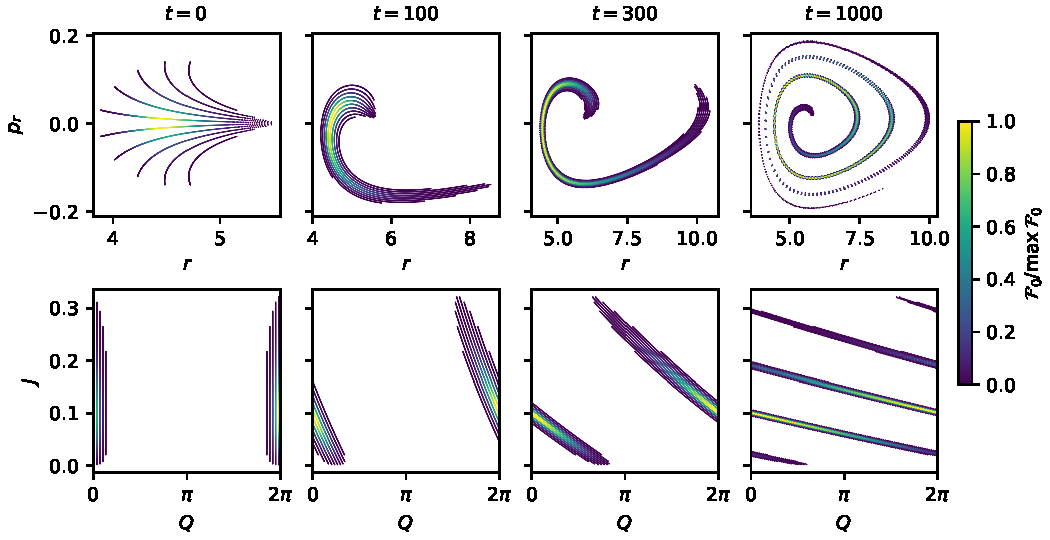
\includegraphics[width=0.85\textwidth]{figuras/validacion_pulso.pdf}}
\caption{Mixing of the initial datum~(\ref{Eq:Pulse}) in the isochrone potential when self-gravity is neglected. Shown are the computational particles in the $(r,p_r)$-plane (upper panels) and in the plane of the action-angle variables (lower panels) at four different times, for a lattice with $N_J\times N_Q = 800\times 64$ points. The color indicates the mass of each particle relative to the largest one, and only particles whose mass exceeds $10^{-3}$ of the latter are shown.}
\label{Fig:Pulse}
\end{figure}

\begin{table}[htp]
\begin{center}
\begin{tabular}{rrl|cccc}
\hline\hline
$N_J$ & $N_Q$ & $\Delta t$ & $e_1$ & $e_2$ & $e_3$ & $e_4$ \\
\hline
$50$ & $64$ & $0.1$ & $4.1\times 10^{-6}$ & $1.6\times 10^{-4}$ & $0.15$ & $0.72$ \\
$100$ & $64$ & $0.1$ & $3.3\times 10^{-8}$ & $1.2\times 10^{-7}$ & $5.1\times 10^{-7}$ & $3.9\times 10^{-6}$ \\
$200$ & $64$ & $0.1$ & $5.3\times 10^{-9}$ & $5.4\times 10^{-9}$ & $5.9\times 10^{-9}$ & $5.5\times 10^{-9}$ \\
$400$ & $64$ & $0.1$ & $5.3\times 10^{-9}$ & $5.5\times 10^{-9}$ & $6.0\times 10^{-9}$ & $5.5\times 10^{-9}$ \\
\hline
$400$ & $16$ & $0.1$ & $9.2\times 10^{-3}$ & $3.7\times 10^{-2}$ & $8.2\times 10^{-2}$ & $0.14$ \\
$400$ & $32$ & $0.1$ & $1.7\times 10^{-5}$ & $7.3\times 10^{-5}$ & $1.8\times 10^{-4}$ & $3.7\times 10^{-4}$ \\
\hline
$400$ & $64$ & $0.2$ & $8.6\times 10^{-8}$ & $8.8\times 10^{-8}$ & $9.6\times 10^{-8}$ & $8.8\times 10^{-8}$ \\
$400$ & $64$ & $0.05$ & $3.3\times 10^{-10}$ & $3.4\times 10^{-10}$ & $3.7\times 10^{-10}$ & $3.4\times 10^{-10}$ \\
$400$ & $64$ & $0.025$ & $2.1\times 10^{-11}$ & $2.0\times 10^{-11}$ & $2.2\times 10^{-11}$ & $2.7\times 10^{-11}$ \\
$400$ & $64$ & exact & $6.6\times 10^{-12}$ & $1.3\times 10^{-11}$ & $2.0\times 10^{-11}$ & $2.7\times 10^{-11}$ \\
\hline\hline
\end{tabular}
\end{center}
\caption{Error $e_n$ defined in Eq.~(\ref{Eq:FreeError}) for the mixing of the initial datum~(\ref{Eq:Pulse}) in the absence of self-gravity, for different lattices and time steps. In the last row the Yoshida integrator is replaced with the exact advance of the angle variables.}
\label{Tab:FreeMixing}
\end{table}

Table~\ref{Tab:FreeMixing} shows the error
\begin{equation}
e_n := \frac{1}{h_0}\max\limits_{0\leq t\leq 2000} \left| h_n(t) - h_n^{exact}(t) \right|
\label{Eq:FreeError}
\end{equation}
for different lattices and time steps. For $N_J\times N_Q = 400\times 64$ and $\Delta t = 0.1$ it does not exceed $6\times 10^{-9}$ for $n\leq 4$. In this case the error is dominated by the time integration. In fact, when the Yoshida integrator is replaced with the exact advance $Q_j\mapsto Q_j + \Omega(J_j)\Delta t$ of the angle variables of the particles, the error drops to less than $3\times 10^{-11}$, and the difference with respect to this solution decreases by the factors $16.0$, $16.0$ and $15.4$ each time $\Delta t$ is halved between $0.2$ and $0.025$ (for $n = 1$), as expected for a fourth-order method.

The remaining rows of Table~\ref{Tab:FreeMixing} show the effect of the lattice. Since the sum~(\ref{Eq:hnPIC}) is a midpoint rule for an integral whose integrand is smooth and, with respect to $Q$, periodic, the error decreases rapidly when $N_J$ or $N_Q$ increase, until it reaches the one of the time integration.

With respect to the angle variable the error of the lattice can be computed explicitly. On a lattice with $N_Q$ points per row the harmonics $n + mN_Q$, $m\in\Integer$, cannot be distinguished from the harmonic $n$, such that the sum over the points $Q_b$ yields $\sum_m (-1)^m\hat{F}_{n+mN_Q}$ instead of $\hat{F}_n$, where the signs are due to the fact that the $Q_b$ are the midpoints of the subintervals. Since the transport does not mix different harmonics, this factor is independent of time. Taking into account that the masses of the computational particles are normalized such that their sum is equal to $M_{gas}$, Eq.~(\ref{Eq:PulseFourier}) gives
\begin{equation}
e_n = \left| \frac{\sum_m (-1)^m I_{n+mN_Q}(z)}{\sum_m (-1)^m I_{mN_Q}(z)} - \frac{I_n(z)}{I_0(z)} \right| ,
\label{Eq:Aliasing}
\end{equation}
where the sums extend over all $m\in\Integer$. This expression reproduces the values in the rows with $N_Q = 16$ and $N_Q = 32$ of Table~\ref{Tab:FreeMixing} to nine significant digits, and for $N_Q = 64$ it is smaller than $5\times 10^{-15}$. Hence, the number of points per row has to be a few times larger than the number $2\sqrt{z}$ of harmonics contained in the DF.

With respect to the action variable the situation is different, since for a given lattice the sum is only reliable over a finite time span. The reason is that the phases $n\Omega(J_a)t$ of two neighboring rows differ by $n|\Omega'(J)|\Delta J\, t$, with $\Delta J$ the spacing between the rows. When this difference reaches $2\pi$ the rows are in phase again, such that $h_n$ exhibits a spurious recurrence~\cite{BirdsallLangdon-Book} at the time
\begin{equation}
t_{rec} = \frac{2\pi}{n|\Omega'(J)|\Delta J}.
\label{Eq:Recurrence}
\end{equation}
In the present example, $\Delta J = 0.6/N_J$ and $|\Omega'(J)|\leq 3/c(L_0)^4\approx 0.088$, which gives $t_{rec}\approx 120\, N_J/n$. For $N_J = 50$ this is $1980$ and $1480$ for $n = 3$ and $n = 4$, respectively, which explains the large values of $e_3$ and $e_4$ in the first row of the table. For the lattices which are used in the following subsections the recurrence time for $n = 1$ exceeds the duration of the simulations: it is $4.7\times 10^4$ for the one of section~\ref{SubSec:ValAA} and at least $1.3\times 10^4$ for those of sections~\ref{SubSec:ValStationarity} and~\ref{SubSec:ValResponse}.

\begin{figure}[htp]
\centerline{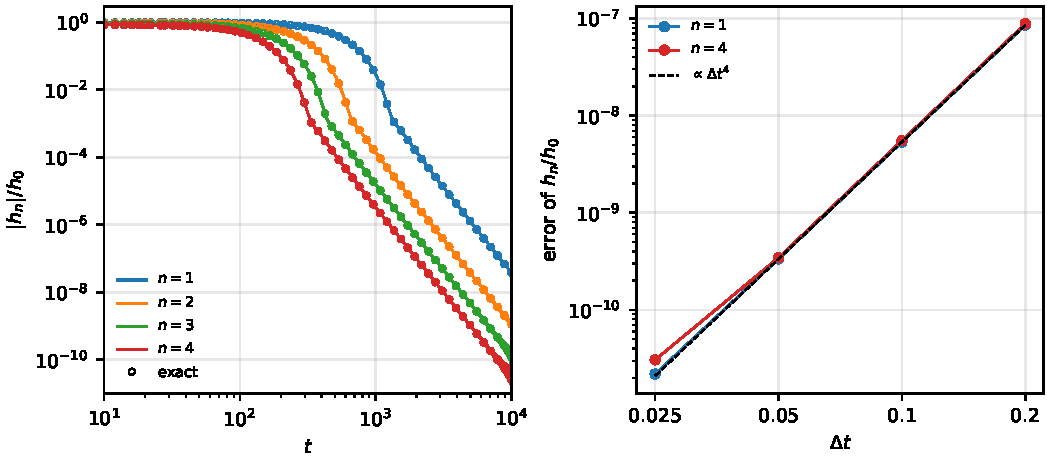
\includegraphics[width=0.85\textwidth]{figuras/validacion_libre.pdf}}
\caption{Left panel: the functions $|h_n(t)|/h_0$, $n = 1,2,3,4$, for the mixing of the initial datum~(\ref{Eq:Pulse}) in the absence of self-gravity, obtained from the PIC code with $N_J\times N_Q = 800\times 64$ and $\Delta t = 0.1$ (solid lines) and from the exact solution~(\ref{Eq:hnFree}) (circles). Right panel: error of the time integration, measured through the difference with the solution in which the angle variables are advanced exactly, as a function of the time step. The dashed line is proportional to $\Delta t^4$.}
\label{Fig:FreeMixing}
\end{figure}

Figure~\ref{Fig:FreeMixing} shows the result of a simulation with $N_J\times N_Q = 800\times 64$ and $\Delta t = 0.1$ which extends to $t = 10^4$. During this time $|h_1|$ and $|h_4|$ decay by seven and ten orders of magnitude, respectively, and the numerical solution reproduces the exact one over the whole range: for $n\leq 4$ the difference does not exceed $6\times 10^{-9} h_0$ at any time, and it is smaller than $2\times 10^{-10} h_0$ for $t\geq 5000$. At late times $|h_n(t)|$ is proportional to $t^{-5}$ (a fit over $5000\leq t\leq 10^4$ gives the exponents $-5.03$ and $-5.01$ for $n = 1$ and $n = 2$). This is the analogue of the algebraic tail~(\ref{Eq:Tail}) for the endpoint $J = 0$ of the support, at which the function $\hat{F}_n B$ vanishes like $J^4$. In the same simulation $h_0$, which is constant for the exact solution, varies by $1.1\times 10^{-9}$, and the total energy by $7\times 10^{-11}$, in relative terms.


\subsection{Action-angle variables of the total potential}
\label{SubSec:ValAA}

As emphasized in section~\ref{SubSec:Observables}, the functions $h_n(t)$ with $n\neq 0$ measure the departure of the gas configuration from a steady state only if they are computed with the action-angle variables which belong to the total potential. To illustrate this point we have repeated the simulation of the previous subsection including the self-gravity of the gas, for $M_{gas}/M = 10^{-4}$, $10^{-3}$ and $10^{-2}$, with $N_J\times N_Q = 400\times 25$, $\Delta r = 0.1$, $\Delta t = 0.1$ and up to $t = 2\times 10^4$, using the weight function~(\ref{Eq:BDef}) with $J_1 = \sigma_1 = 0.1$. The initial datum~(\ref{Eq:Pulse}), which is defined in terms of the action-angle variables of the external potential, is far from a steady state, and the gas undergoes mixing while its potential $\Phi_{gas}$ readjusts: for $M_{gas}/M = 10^{-3}$ it changes by up to $40$ percent of its largest value between $t = 0$ and $t = 2000$, and afterwards it is stationary up to fluctuations whose root mean square is smaller than $10^{-3}$ of this value.

\begin{figure}[htp]
\centerline{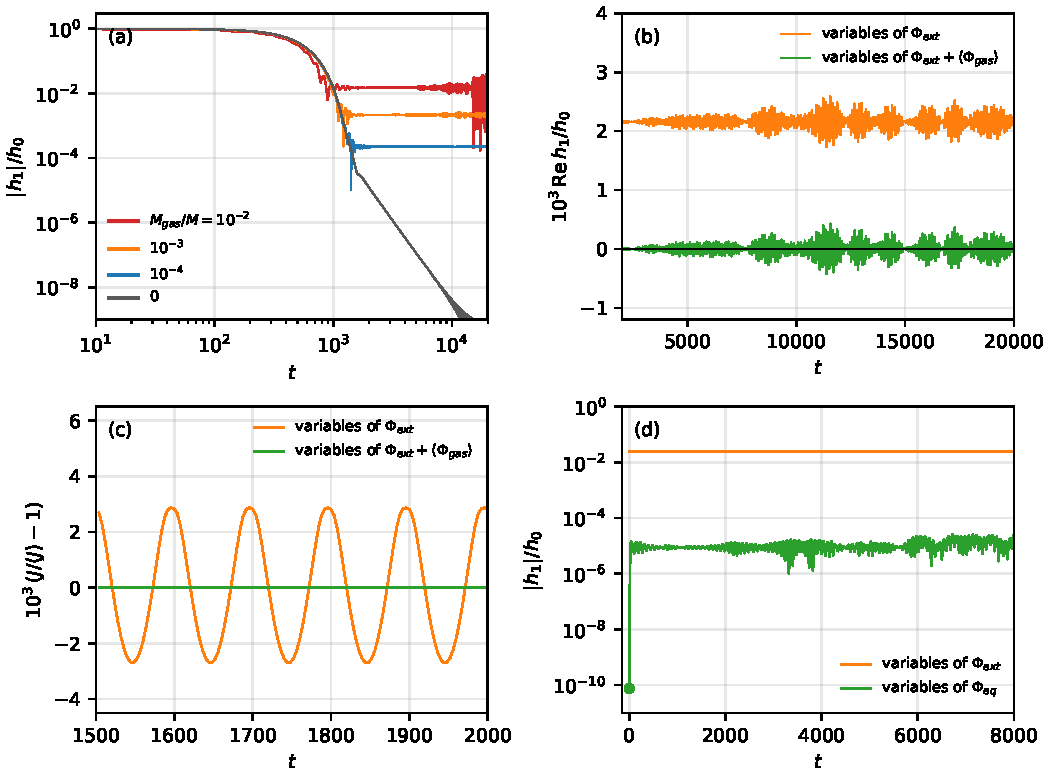
\includegraphics[width=0.85\textwidth]{figuras/validacion_mapa.pdf}}
\caption{Dependency of the function $h_1$ on the action-angle variables which are used to compute it. (a) $|h_1|/h_0$ for the mixing of the initial datum~(\ref{Eq:Pulse}) including self-gravity, computed with the action-angle variables of the external potential, for different masses of the gas. (b) Real part of $h_1/h_0$ for $M_{gas}/M = 10^{-3}$, computed with the action-angle variables of the external potential and with those of the potential $\Phi_{ext} + \langle\Phi_{gas}\rangle$, where $\langle\Phi_{gas}\rangle$ is the average of $\Phi_{gas}$ over $t\geq 2000$. (c) Relative variation of the action variable of a single computational particle for the same mass, for both sets of variables; here $\langle\Phi_{gas}\rangle$ is the average over $1500\leq t\leq 2000$, and $\langle J\rangle$ denotes the mean value over this interval. (d) $|h_1|/h_0$ for the reference simulation of the polytrope with $k = 2$ and $M_{gas}/M = 0.01$ in the Kepler potential, computed with the action-angle variables of the external potential and with those of $\Phi_{eq}$.}
\label{Fig:Map}
\end{figure}

Figure~\ref{Fig:Map}(a) shows the function $|h_1(t)|/h_0$ which is obtained with the action-angle variables of the external potential. When self-gravity is neglected it decays according to the law $t^{-5}$ found in the previous subsection, until it reaches the level of the numerical errors, which is of the order of $10^{-9}$, at $t\approx 10^4$. In contrast to this, when self-gravity is taken into account it settles down to a plateau: the magnitude of the time average of $h_1/h_0$ over the interval $2000\leq t\leq 2\times 10^4$ is $2.2\times 10^{-4}$, $2.2\times 10^{-3}$ and $1.5\times 10^{-2}$ for the three values of $M_{gas}/M$, whereas it is $9\times 10^{-9}$ in the absence of self-gravity. For $M_{gas}/M = 10^{-3}$ the same value, $2.16\times 10^{-3}$, is obtained with $N_J\times N_Q = 800\times 25$ and $400\times 50$. Such a plateau could be mistaken for a collective mode which is not damped.

However, the plateau disappears when the same particle data are analyzed with the action-angle variables of the potential $\Phi_{ext} + \langle\Phi_{gas}\rangle$, where $\langle\Phi_{gas}\rangle$ denotes the time average of the potential of the gas after it has become stationary. This is shown in Fig.~\ref{Fig:Map}(b) for $M_{gas}/M = 10^{-3}$: with these variables $h_1/h_0$ fluctuates about zero instead of about the value $2.16\times 10^{-3}$, and the magnitude of its time average over $2000\leq t\leq 2\times 10^4$ is reduced to $5.4\times 10^{-7}$, which is $4000$ times smaller. Therefore, the plateau is due to the choice of the coordinates and not to the dynamics. The reason is that the action variable of the external potential is not conserved along the trajectories of the gas particles in the total potential. As shown in Fig.~\ref{Fig:Map}(c), for a given particle it oscillates with the period of the radial motion; the relative difference between its largest and its smallest value is $5.6\times 10^{-3}$ for the particle shown, which has $J = 0.10$, and $4.4\times 10^{-3}$ for a particle with $J = 0.30$. In contrast to this, the action variable which belongs to the total potential is constant to within a relative variation of $2\times 10^{-5}$. Consequently, a DF which depends only on the action variable of the total potential is not independent of the angle variable of the external one, the difference between both sets of variables being of the first order in $M_{gas}/M$.

What remains after subtracting the time average is a fluctuation which is the same for both sets of variables, see Fig.~\ref{Fig:Map}(b). Its root mean square is $2.0\times 10^{-4} h_0$ in the simulation with $400\times 25$ particles, and $1.1\times 10^{-4} h_0$ and $9.6\times 10^{-5} h_0$ in those with $800\times 25$ and $400\times 50$ particles, respectively. For $M_{gas}/M = 10^{-2}$ it grows in time and is visible in Fig.~\ref{Fig:Map}(a) for $t > 10^4$; in this case its root mean square is $9.1\times 10^{-3} h_0$ with $400\times 25$ particles and $2.2\times 10^{-3} h_0$ with $800\times 25$ particles. Hence, these fluctuations are caused by the finite number of particles, which is the subject of the next subsection.

The same occurs for a self-consistent steady state. Figure~\ref{Fig:Map}(d) shows the result for the reference simulation of the polytrope~(\ref{Eq:Polytrope}) with $k = 2$ and $M_{gas}/M = 0.01$ in the Kepler potential, which is analyzed in section~\ref{Sec:FixedL}, with the weight function~(\ref{Eq:BDef}) with $J_1 = 0.35$ and $\sigma_1 = 0.2$. The value of $|h_1|/h_0$ which is obtained with the action-angle variables of the external potential is $2.4\times 10^{-2}$ at all times, whereas with those of $\Phi_{eq}$ it is $7.5\times 10^{-11}$ at $t = 0$ and remains below $3\times 10^{-5}$ up to $t = 8000$. The small value which develops for $t > 0$ reflects the departure of the discretized steady state from stationarity, which is analyzed next.


\subsection{Stationarity of the discretized steady states}
\label{SubSec:ValStationarity}

Next, we analyze the reference simulations with $\varepsilon = 0$, in which the gas should remain in the self-consistent steady state. We consider the polytrope~(\ref{Eq:Polytrope}) with $k = 1.25$, $L_0 = 2$ and $J_{max} = 0.7$ in the Kepler potential with $M_{gas}/M = 1$, which is the largest mass ratio considered in these notes and, hence, the most demanding case, and the weight function~(\ref{Eq:BDef}) with $J_1 = 0.35$ and $\sigma_1 = 0.2$. We use two quantities to measure the departure from stationarity. The first one is $|h_1^{(0)}(t)|/h_0$, which vanishes for a steady state, and the second one is the root mean square displacement of the action variables of the computational particles,
\begin{equation}
\Delta J_{rms}(t) := \left[ \frac{1}{M_{gas}}\sum\limits_{j=1}^N m_j\left( J_j(t) - J_j(0) \right)^2 \right]^{1/2},
\label{Eq:DeltaJrms}
\end{equation}
both being computed with the action-angle variables of $\Phi_{eq}$. The results for three different numbers of particles and two values of $\Delta r$ are shown in Table~\ref{Tab:Reference} and Fig.~\ref{Fig:Reference}. They reveal two different effects.

\begin{table}[htp]
\begin{center}
\begin{tabular}{lll|ccccc|ccc|c}
\hline\hline
 & & & \multicolumn{5}{c|}{$10^3\, |h_1^{(0)}|/h_0$} & \multicolumn{3}{c|}{$10^3\,\Delta J_{rms}/J_{max}$} & \\
$N_J\times N_Q$ & $\Delta r$ & $\Delta t$ & $t = 0$ & $500$ & $1000$ & $2000$ & $3900$ & $t = 1000$ & $2000$ & $4000$ & $|\Delta\mathcal{E}_{gas}/\mathcal{E}_{gas}|$ \\
\hline
$400\times 25$ & $0.1$ & $0.1$ & $1.8$ & $1.5$ & $1.5$ & $2.3$ & $10.7$ & $1.4$ & $6.3$ & $37$ & $7.7\times 10^{-6}$ \\
$400\times 25$ & $0.05$ & $0.1$ & $0.72$ & $0.44$ & $1.4$ & $2.1$ & $12.3$ & $1.7$ & $9.8$ & $42$ & $2.7\times 10^{-6}$ \\
$800\times 50$ & $0.1$ & $0.1$ & $2.0$ & $1.4$ & $1.4$ & $1.5$ & $1.7$ & $0.50$ & $0.58$ & $2.5$ & $3.0\times 10^{-6}$ \\
$1280\times 80$ & $0.1$ & $0.05$ & $2.0$ & $1.4$ & $1.4$ & $1.4$ & $1.4$ & $0.46$ & $0.41$ & $0.56$ & $1.9\times 10^{-6}$ \\
\hline\hline
\end{tabular}
\end{center}
\caption{Departure from stationarity of the reference simulations ($\varepsilon = 0$) for the polytrope with $k = 1.25$ and $M_{gas}/M = 1$ in the Kepler potential. For $|h_1^{(0)}|/h_0$ we give the largest value in the interval $[t,t+100]$. The last column is the largest relative change of the total energy up to $t = 4000$.}
\label{Tab:Reference}
\end{table}

\begin{figure}[htp]
\centerline{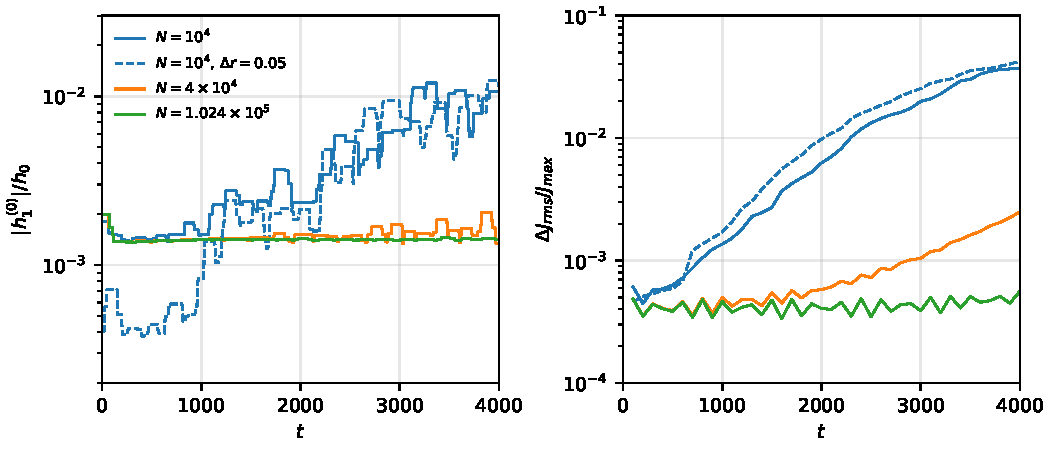
\includegraphics[width=0.85\textwidth]{figuras/validacion_referencia.pdf}}
\caption{Reference simulations ($\varepsilon = 0$) for the polytrope with $k = 1.25$ and $M_{gas}/M = 1$ in the Kepler potential, for different numbers $N = N_J N_Q$ of particles and grid spacings ($\Delta r = 0.1$ unless otherwise stated). Left panel: largest value of $|h_1^{(0)}|/h_0$ in a moving window of width $100$. Right panel: root mean square displacement~(\ref{Eq:DeltaJrms}) of the action variables of the particles.}
\label{Fig:Reference}
\end{figure}

The first effect is present from the beginning. Within the first radial periods, $|h_1^{(0)}|/h_0$ rises to a level of about $1.4$ to $2\times 10^{-3}$, which does not depend on the number of particles and is reduced by a factor between $2.5$ and $3.4$ when $\Delta r$ is halved. Its origin is the discretization error of the potential: the lattice represents a steady state of the exact potential $\Phi_{eq}$, whereas the particles move in the potential computed on the grid, which differs from $\Phi_{eq}$ by an error of the order of $\Delta r^2$. Hence, the initial configuration is slightly out of equilibrium, and the gas reacts to this. We have verified the scaling with $\Delta r$ for the Wilson model with $W_0 = 3$, $J_{max} = 0.138$ and $M_{gas}/M = 0.5$ in the isochrone potential. In this case, the root mean square over the interval $3\leq r\leq 15$ of $\delta\Phi^{(0)}$ at $t = 0$, of its time average and of the remaining oscillation, which has the frequency of the oscillating mode of this steady state, are $8.7\times 10^{-5}$, $1.7\times 10^{-4}$ and $7.7\times 10^{-5}$ in units of the largest value of $|\Phi_{gas}|$ for $\Delta r = 0.1$. They change by less than three percent when the number of particles is multiplied by four or the time step is halved, and they decrease by the factors $4.0$, $4.0$ and $3.9$ when $\Delta r$ is halved. Since this error is the same in the simulation with the perturbation and in its reference simulation, to leading order it cancels in the response~(\ref{Eq:Response}).

The second effect is a growth which sets in after a certain time. For $N = 10^4$ the quantity $|h_1^{(0)}|/h_0$ starts to grow at $t\approx 1000$ and reaches $10^{-2}$ at the end of the simulation, while the displacement of the action variables increases from $1.4\times 10^{-3} J_{max}$ at $t = 1000$ to $3.7\times 10^{-2} J_{max}$ at $t = 4000$. This growth is not reduced by halving $\Delta r$ (in fact, it becomes slightly faster), but it is delayed when the number of particles is increased: for $N = 4\times 10^4$ the displacement stays below $6\times 10^{-4} J_{max}$ up to $t = 2000$ and reaches $2.5\times 10^{-3} J_{max}$ at $t = 4000$, and for $N = 1.024\times 10^5$ both quantities remain constant up to $t = 4000$. Therefore, it is due to the discreteness of the particles, which gradually destroys the regularity of the lattice. Note that the dependency on $N$ is much stronger than the one of the fluctuations of a random sample, which are proportional to $N^{-1/2}$. The total energy is conserved to better than $10^{-5}$ in all cases; its error decreases when $\Delta r$ is reduced or $N$ is increased, but it does not depend on $\Delta t$ (see the next subsection).

For a gas of small mass the lattice is preserved over much longer times: for the polytrope with $k = 2$ and $M_{gas}/M = 0.01$ and $N = 10^4$ we find $\Delta J_{rms} = 3.6\times 10^{-5} J_{max}$ at $t = 8000$. We conclude that for $M_{gas}/M = 1$ the quiet start with $N = 10^4$ particles is reliable up to $t\approx 1000$, whereas $N\geq 4\times 10^4$ particles are required for the time span $t\leq 4000$ of our simulations.

Finally, we mention a test of the computation of the gravitational field in a situation which is dominated by self-gravity, namely the collapse of a cold homogeneous sphere of mass $M_{gas}$ and radius $R$ in the absence of an external potential. Since in this case all the particles have $L = 0$, this test has been performed with an implementation of the same algorithm for a general distribution of the angular momenta. Before the shells cross each other, the shell with initial radius $r_0$ follows the cycloid $r = r_0\cos^2\theta$, $t = (\theta + \sin\theta\cos\theta)/\sqrt{2GM_{gas}/R^3}$. For $\Delta r = 0.01 R$, the median of the relative error of the radii of the shells with $0.1 < r_0/R < 0.9$ at the time $t = 0.8\sqrt{R^3/(GM_{gas})}$ is $1.8\times 10^{-5}$ for $N = 200$ and $4.3\times 10^{-6}$ for $N = 400$ shells, which corresponds to second-order convergence in $1/N$.


\subsection{Time step, amplitude of the perturbation and comparison with the linearized equations}
\label{SubSec:ValResponse}

We now turn to the response~(\ref{Eq:Response}) of the gas to a perturbation of the form~(\ref{Eq:InitialData}). We first analyze its dependency on the time step. To this purpose we consider the polytrope with $k = 1$ and $M_{gas}/M = 1$ in the Kepler potential (with the remaining parameters as in the previous subsection), $\varepsilon = 0.1$, $N_J\times N_Q = 400\times 25$ and $\Delta r = 0.1$, and we repeat the simulation and its reference simulation with $\Delta t = 0.2$, $0.1$ and $0.05$. Figure~\ref{Fig:TimeStep} shows the difference between the responses $\delta\Phi_{res}$ which are obtained with different time steps, measured with the norm~(\ref{Eq:deltaPhiNorm}) for $r_a = 3$ and $r_b = 7.5$. In the intervals $0\leq t\leq 250$, $250\leq t\leq 500$, $500\leq t\leq 750$ and $750\leq t\leq 1000$, the difference between the results for $\Delta t = 0.1$ and $\Delta t = 0.05$, relative to the largest value of $\|\delta\Phi_{res}\|$ in the respective interval, is at most $6.6\times 10^{-4}$, $3.0\times 10^{-3}$, $5.6\times 10^{-3}$ and $1.9\times 10^{-2}$, and the one between $\Delta t = 0.2$ and $\Delta t = 0.05$ is larger by the factors $4.4$, $5.0$, $6.4$ and $6.3$. For a second-order method one expects the factor five, and for a fourth-order one the factor $17$. The same conclusion is obtained from the simulation with $\varepsilon = 0.1$ alone, for which we have a further run with $\Delta t = 0.025$: relative to the latter, the error of the potential for $\Delta t = 0.05$ is smaller than the one for $\Delta t = 0.1$ by the factors $4.7$, $4.1$, $3.9$ and $3.4$ in the same intervals, where again the factor five is expected for a second-order method. Hence, in the presence of self-gravity the time integration is only second-order accurate, in contrast to the fourth-order convergence found in section~\ref{SubSec:ValFree}. This reduction of the order is to be expected, since the field which results from the linear weights~(\ref{Eq:Deposit}) is continuous but not differentiable with respect to the positions of the particles, whereas the fourth-order accuracy of the composition method requires a smooth force.

\begin{figure}[htp]
\centerline{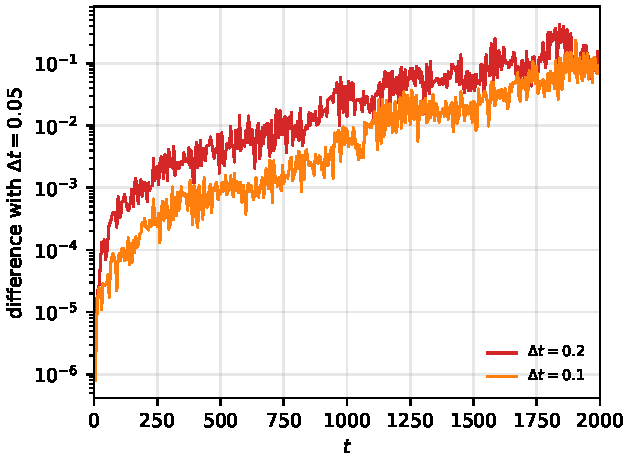
\includegraphics[width=0.5\textwidth]{figuras/validacion_paso.pdf}}
\caption{Dependency of the response on the time step for the polytrope with $k = 1$ and $M_{gas}/M = 1$ in the Kepler potential, with $\varepsilon = 0.1$ and $N = 10^4$. Shown is the norm~(\ref{Eq:deltaPhiNorm}) of the difference between the response $\delta\Phi_{res}$ obtained with the indicated time step and the one obtained with $\Delta t = 0.05$, divided by the largest value of $\|\delta\Phi_{res}\|$.}
\label{Fig:TimeStep}
\end{figure}

The error due to the time step grows with time. For $\Delta t = 0.1$ it amounts to two percent of the response at $t = 1000$. At later times the differences between the three simulations grow to several ten percent. However, this is not a consequence of the time integration: at $t = 2000$ the radii of corresponding particles in the simulations with $\Delta t = 0.1$ and $\Delta t = 0.025$ differ by up to $3.3$, which shows that for $N = 10^4$ the trajectories of the individual particles are no longer correlated, in accordance with the loss of the quiet start at $t\approx 1000$ found in the previous subsection. In contrast to this, the frequency of the oscillation of $\delta\Phi_{res}$, determined from its periodogram over $500\leq t\leq 2000$, is $0.14770$ for the three time steps, and the relative error of the total energy, $1.8\times 10^{-5}$, is the same for $\Delta t = 0.2$, $0.1$, $0.05$ and $0.025$, such that it is not due to the time integration.

Next, we compare the response with the solution of the linearized equations obtained with the method of section~\ref{SubSec:LinSolver}. For a gas of small mass we consider the polytropes with $k = 0.75$, $1$, $1.5$ and $2$ and $M_{gas}/M = 0.01$ in the Kepler potential, with $N_J\times N_Q = 400\times 25$, $\Delta r = 0.1$ and $\Delta t = 0.1$. In these cases the response decays algebraically (see section~\ref{Sec:FixedL}): at $t = 1000$ the magnitude of $\chi_1$ has decreased to a fraction between $2.6\times 10^{-3}$ (for $k = 0.75$) and $1.8\times 10^{-4}$ (for $k = 2$) of its initial value. With $\varepsilon = 0.1$, the difference between the function $\chi_1(t)$ obtained from the PIC code and the one obtained from the linearized equations is smaller than $1.2\times 10^{-4}|\chi_1(0)|$ for all $0\leq t\leq 2000$ and the four values of $k$. Relative to the largest value of $|\chi_1|$ in the respective interval, it is at most $1.2\times 10^{-4}$ for $0\leq t\leq 500$ and between $0.3$ and $0.5$ percent for $500\leq t\leq 1000$. With $\varepsilon = 0.5$ the corresponding numbers are $5\times 10^{-4}$ and $1.4$ percent. Therefore, for this mass ratio the two methods, which are based on entirely different discretizations, agree with each other to better than one percent while the response decays by more than two orders of magnitude, and the dependency on the amplitude of the perturbation is weak.

For $M_{gas}/M = 1$ the situation is different, since the response depends on $\varepsilon$ even for rather small amplitudes. We consider again the polytrope with $k = 1.25$, for which the linearized equations predict an oscillating mode (see section~\ref{Sec:FixedL}), and compare three simulations with $\varepsilon = 0.1$, $0.03$ and $0.01$ which share the lattice with $N_J\times N_Q = 1280\times 80$ points, the time step $\Delta t = 0.05$ and the reference simulation, such that they only differ from each other in the amplitude. In order to compare two oscillating signals we use the quantity
\begin{equation}
\kappa(t_0) := \frac{\sum_j w(t_j - t_0)\,\chi_1(t_j)\,\chi_1^{lin}(t_j)^*}{\sum_j w(t_j - t_0)\,|\chi_1^{lin}(t_j)|^2},\qquad
w(\tau) := \cos^2\left( \frac{\pi\tau}{T_w} \right)\quad\hbox{for $|\tau|\leq \frac{T_w}{2}$},
\label{Eq:kappa}
\end{equation}
and $w(\tau) := 0$ otherwise, where $\chi_1^{lin}$ refers to the solution of the linearized equations, the sums extend over the output times $t_j$ which are common to both solutions, and $T_w = 200$, which corresponds to about five periods of the oscillation. The magnitude of $\kappa(t_0)$ is the ratio between the amplitudes of the two signals in the window centered at $t_0$, and its phase is their phase difference, such that $-d\arg\kappa/dt_0$ is the difference between their frequencies. Since $\kappa$ depends linearly on $\chi_1$, it can be extrapolated to $\varepsilon = 0$.

\begin{table}[htp]
\begin{center}
\begin{tabular}{l|cccccc}
\hline\hline
$\varepsilon$ & $t_0 = 500$ & $1000$ & $1500$ & $2000$ & $2500$ & $3000$ \\
\hline
$0.1$ & $0.869$ & $0.614$ & $0.591$ & $0.762$ & $0.913$ & $0.830$ \\
$0.03$ & $0.976$ & $0.946$ & $0.923$ & $0.908$ & $0.924$ & $0.906$ \\
$0.01$ & $0.992$ & $0.990$ & $0.986$ & $0.978$ & $1.004$ & $0.997$ \\
\hline
$0$ (linear) & $1.000$ & $1.013$ & $1.020$ & $1.017$ & $1.048$ & $1.048$ \\
$0$ (quadratic) & $0.997$ & $1.004$ & $1.017$ & $1.024$ & $1.064$ & $1.063$ \\
\hline\hline
\end{tabular}
\end{center}
\caption{The ratio $|\kappa(t_0)|$ between the amplitudes of the response obtained from the PIC code and from the linearized equations, see Eq.~(\ref{Eq:kappa}), for the polytrope with $k = 1.25$ and $M_{gas}/M = 1$ in the Kepler potential and three amplitudes of the perturbation ($N = 1.024\times 10^5$, $\Delta t = 0.05$). The last two rows refer to the extrapolation to $\varepsilon = 0$ by means of a straight line through the results for $\varepsilon = 0.01$ and $0.03$ and of a parabola through the three results, respectively.}
\label{Tab:Amplitude}
\end{table}

The results are shown in Table~\ref{Tab:Amplitude}. For $\varepsilon = 0.1$ the amplitude of the response falls to $56$ percent of the one predicted by the linearized equations at $t_0 = 1300$, and for $\varepsilon = 0.03$ to $91$ percent at $t_0 = 2000$, whereas for $\varepsilon = 0.01$ it stays between $0.977$ and $1.005$ of the latter for $t_0\leq 2000$ and between $0.95$ and $1.06$ up to $t_0 = 3900$. The simulation with $\varepsilon = 0.1$, $N = 10^4$ and $\Delta t = 0.1$ gives $|\kappa| = 0.871$ and $0.629$ at $t_0 = 500$ and $1000$, such that for as long as its quiet start lasts it agrees with the one with $N = 1.024\times 10^5$ to within two percent. Hence, the loss of amplitude is not a numerical artifact but a nonlinear effect; its origin is discussed in section~\ref{Sec:FixedL}. Extrapolating the three results to $\varepsilon = 0$ we obtain an amplitude which lies between $1.00$ and $1.05$ times the linear one for $t_0\leq 2000$ when a straight line through the two smallest amplitudes is used, and between $0.99$ and $1.06$ when a parabola through the three amplitudes is used. For $250\leq t_0\leq 2000$ the phase of $\kappa$ grows linearly with $t_0$, at the rate $1.3\times 10^{-4}$ for $\varepsilon = 0.03$ and $5.8\times 10^{-5}$ for $\varepsilon = 0.01$, which means that the frequency of the oscillation decreases slightly with the amplitude. For the extrapolation to $\varepsilon = 0$ the rate is $2.5\times 10^{-5}$ (straight line) and $0.7\times 10^{-5}$ (parabola), which is of the order of the accuracy with which the frequency of the linearized solution is known (see the next subsection). Finally, for $\varepsilon = 0.01$ the fluctuations of $\kappa$ between consecutive windows are of the order of one percent for $t_0\leq 2000$ and of four percent afterwards. Note that for this amplitude the function $h_1^{(0)}/\varepsilon$ of the reference simulation is $2.5$ times larger than the response itself, such that the latter is obtained as the difference of two much larger quantities.

We conclude that for $M_{gas}/M = 1$ the PIC code reproduces the solution of the linearized equations within a few percent, provided that $N\approx 10^5$ particles and amplitudes $\varepsilon\leq 0.01$ are used. \EJ{For $k = 0.75$, $1$ and $2$ the simulations of section~\ref{Sec:FixedL} with $M_{gas}/M = 1$ still have $N = 10^4$ particles and $\varepsilon = 0.1$. The ones with $N = 1.024\times 10^5$, $\Delta t = 0.05$ and $\varepsilon = 0.03$ and $0.1$ have been run on the cluster and their analysis is pending; the default parameters quoted at the end of section~\ref{SubSec:PIC} have to be adapted accordingly.}


\subsection{Linearized equations and gain of the self-consistent loop}
\label{SubSec:ValLinear}

In order to estimate the accuracy of the solutions of the linearized equations, we have repeated the computation for the polytrope with $k = 1.25$ and $M_{gas}/M = 1$ of the previous subsection with half the time step, with twice the number of points in $Q$ and with twice the number of rows in $J$, and compared the results with the one for the default values $N_J\times N_Q = 1600\times 32$ and $\Delta t = 0.5$ by means of the quantity~(\ref{Eq:kappa}) in the interval $300\leq t_0\leq 3900$. Halving $\Delta t$ changes the amplitude of $\chi_1$ by $0.2$ percent and its frequency by $-0.9\times 10^{-5}$, doubling $N_Q$ changes them by $-0.3$ percent and $1.4\times 10^{-5}$, and doubling $N_J$ by $0.01$ percent and $0.7\times 10^{-6}$, respectively. Since the differences in the frequency accumulate in the phase, the difference between the functions $\chi_1(t)$ themselves grows linearly in time; at $t = 4000$ it reaches $3.5$, $5.9$ and $0.3$ percent of the amplitude in the three cases.

An independent test is provided by the gain $\lambda(\omega)$, which is computed by a completely different method (see section~\ref{SubSec:GainNum}). For the polytropes with $k = 0.75$, $1$ and $1.25$ and $M_{gas}/M = 1$ in the Kepler potential, the solution of the linearized equations settles down to an oscillation whose frequency, determined with the method of section~\ref{SubSec:Fits} in the window $300\leq t\leq 1500$, is $0.14169$, $0.14783$ and $0.15330$, respectively, whereas the equation $\lambda(\omega_d) = 1$ yields $\omega_d = 0.14169$, $0.14785$ and $0.15326$. Hence, both methods agree to within $4\times 10^{-5}$.




%%%%%%%%%%%%%%%%%%%%%%%%%%%%%%%%%%%%%%%%%%%%%
\section{Results}
\label{Sec:FixedL}
%%%%%%%%%%%%%%%%%%%%%%%%%%%%%%%%%%%%%%%%%%%%%

In this section we apply the methods of section~\ref{Sec:Numerics} to the reduced model in which all the gas particles have the same magnitude $L_0$ of the angular momentum. We start with the two families of self-consistent steady states whose perturbations are analyzed, and with the dependency of their frequency bands on the mass of the gas. Next, we compute the gain $\lambda(\omega)$ of the self-consistent loop, verify its behavior at the edge of the band, and determine the threshold mass above which an oscillating mode exists. Then, we analyze the response of the gas to the perturbation~(\ref{Eq:InitialData}), first below the threshold, where it decays, and afterwards above it, where it settles down to an oscillation which is not damped, and in each case we compare the results which are obtained from the PIC code, from the linearized equations and from the gain. Finally, we show that the dependency of the response on the amplitude of the perturbation which was found in section~\ref{SubSec:ValResponse} is due to the trapping of the gas particles near the edge of the steady state by the oscillating mode, and we estimate the amplitude above which this occurs.


\subsection{Steady states}
\label{SubSec:FixedLStates}

We consider the two families of self-consistent steady states introduced in section~\ref{SubSec:SteadyStatesNum}. The first one consists of the lowered Maxwellians~(\ref{Eq:LoweredMaxwellian}) with $W_0 = 3$ in the isochrone potential, for $L_0 = 2$. Unless otherwise stated we choose $g = 2$ and $J_{max} = 0.138$, and we vary the mass of the gas in the range $0.003\leq M_{gas}/M\leq 0.5$. In the limit $M_{gas}/M\to 0$, Eq.~(\ref{Eq:OmegaIsochrone}) with $c(L_0) = 1 + \sqrt{2}$ yields the frequency band $[\Omega_{min},\Omega_{max}] = [0.0602,0.0711]$, whose width is only $17$ percent of its mean value, and the gas occupies the shell $4.3 < r < 8.5$. In order to analyze the dependency of the results on the width of the band and on the behavior of the DF at the edge of its support, we also consider $J_{max} = 0.083$ and $J_{max} = 0.276$, as well as the exponents $g = 0.75$, $1$, $1.5$ and $3$.

The second family consists of the polytropes~(\ref{Eq:Polytrope}) in the Kepler potential with $k = 0.75$, $1$, $1.25$, $1.5$, $2$ and $3$, for $L_0 = 2$, $J_{max} = 0.7$ and $0.01\leq M_{gas}/M\leq 1$. These are the steady states for which the dichotomy of Ref.~\cite{mHgRmScS25} has been established. Recall that in the Kepler case the value of $L_0$ can be fixed by means of the rescaling~(\ref{Eq:Rescaling}), such that this family is characterized by $k$, $J_{max}/L_0$ and $M_{gas}/M$. In the limit $M_{gas}/M\to 0$ the frequency band is $[0.0508,0.125]$ and the gas occupies the shell $2.4 < r < 12.2$. Hence, in contrast to the first family, the band is wide: $\Omega_{max}/\Omega_{min} = 2.46$.

\begin{table}[htp]
\begin{center}
\begin{tabular}{ll|cc|cc|cc}
\hline\hline
 & $M_{gas}/M$ & $r_{in}$ & $r_{out}$ & $\Omega_{min}$ & $\Omega_{max}$ & $\lambda(0)$ & $\lambda_{edge}$ \\
\hline
lowered Maxwellian, $g = 2$ & $0.0065$ & $4.31$ & $8.50$ & $0.06097$ & $0.07230$ & $0.018$ & $0.100$ \\
 & $0.042$ & $4.25$ & $8.29$ & $0.06548$ & $0.07915$ & $0.105$ & $0.555$ \\
 & $0.058$ & $4.23$ & $8.20$ & $0.06756$ & $0.08230$ & $0.140$ & $0.720$ \\
 & $0.075$ & $4.20$ & $8.11$ & $0.06979$ & $0.08570$ & $0.174$ & $0.874$ \\
 & $0.097$ & $4.17$ & $7.99$ & $0.07271$ & $0.09017$ & $0.215$ & $1.047$ \\
 & $0.17$ & $4.06$ & $7.63$ & $0.08275$ & $0.10552$ & $0.326$ & $1.468$ \\
 & $0.5$ & $3.60$ & $6.40$ & $0.13419$ & $0.18434$ & $0.586$ & $2.210$ \\
\hline
polytrope, $k = 0.75$ & $0.01$ & $2.39$ & $12.10$ & $0.05159$ & $0.12618$ & $0.008$ & $\infty$ \\
\phantom{polytrope,} $k = 1$ & $0.01$ & $2.39$ & $12.10$ & $0.05161$ & $0.12626$ & $0.008$ & $\infty$ \\
\phantom{polytrope,} $k = 1.5$ & $0.01$ & $2.39$ & $12.10$ & $0.05163$ & $0.12640$ & $0.009$ & $0.018$ \\
\phantom{polytrope,} $k = 2$ & $0.01$ & $2.39$ & $12.09$ & $0.05165$ & $0.12652$ & $0.010$ & $0.016$ \\
\hline
polytrope, $k = 0.75$ & $1$ & $1.83$ & $7.57$ & $0.15159$ & $0.28367$ & $0.387$ & $\infty$ \\
\phantom{polytrope,} $k = 1$ & $1$ & $1.81$ & $7.50$ & $0.15399$ & $0.29366$ & $0.402$ & $\infty$ \\
\phantom{polytrope,} $k = 1.25$ & $1$ & $1.80$ & $7.45$ & $0.15601$ & $0.30303$ & $0.415$ & $1.583$ \\
\phantom{polytrope,} $k = 1.5$ & $1$ & $1.79$ & $7.40$ & $0.15774$ & $0.31186$ & $0.428$ & $1.051$ \\
\phantom{polytrope,} $k = 2$ & $1$ & $1.78$ & $7.32$ & $0.16053$ & $0.32814$ & $0.452$ & $0.820$ \\
\phantom{polytrope,} $k = 3$ & $1$ & $1.75$ & $7.21$ & $0.16434$ & $0.35648$ & $0.492$ & $0.738$ \\
\hline\hline
\end{tabular}
\end{center}
\caption{Properties of the self-consistent steady states of the reduced model whose perturbations are analyzed in this section: the lowered Maxwellians~(\ref{Eq:LoweredMaxwellian}) with $W_0 = 3$ and $J_{max} = 0.138$ in the isochrone potential, and the polytropes~(\ref{Eq:Polytrope}) with $J_{max} = 0.7$ in the Kepler potential, in both cases with $L_0 = 2$. Shown are the inner and outer radii of the shell which is occupied by the gas, the frequency band, and the gain of the self-consistent loop at zero frequency and at the edge of the band.}
\label{Tab:SteadyStates}
\end{table}

The properties of the steady states to which the simulations of this section refer are summarized in Table~\ref{Tab:SteadyStates}. As the mass of the gas increases, the potential well becomes deeper, the gas contracts, and the frequencies of all the orbits grow. For the lowered Maxwellians, $\Omega_{min}$ increases from $0.0605$ for $M_{gas}/M = 0.003$ to $0.134$ for $M_{gas}/M = 0.5$, and the ratio $\Omega_{max}/\Omega_{min}$ from $1.18$ to $1.37$. For the polytropes with $M_{gas}/M = 1$, $\Omega_{min}$ is about three times larger than for vanishing mass, and $\Omega_{max}/\Omega_{min}$ lies between $1.87$ and $2.17$.

For all these steady states the DF is a decreasing function of the energy, such that the considerations of section~\ref{SubSec:Gain} apply. The gain at zero frequency increases with the mass of the gas (see Table~\ref{Tab:SteadyStates}); its largest value, $\lambda(0) = 0.586$, is attained for the lowered Maxwellian with $M_{gas}/M = 0.5$. Therefore, all the steady states considered here are linearly stable with respect to spherically symmetric perturbations. Furthermore, the second largest eigenvalue of the operator $S(\omega)$, which also increases with $\omega$, is smaller than $0.26$ in all the cases. Its largest value at the edge of the band, $0.258$, is again attained for the lowered Maxwellian with $M_{gas}/M = 0.5$. For the steady states with $k\leq 1$, for which the largest eigenvalue diverges at the edge, we have evaluated the second one up to the distance $10^{-12}(\Omega_{max} - \Omega_{min})$ from the edge, where it is equal to $0.230$ and $0.246$ for the polytropes with $M_{gas}/M = 1$ and $k = 0.75$ and $k = 1$, respectively. Hence, there is at most one oscillating mode with frequency below the band.

In the remainder of this section the response of the gas to the perturbation~(\ref{Eq:InitialData}) is described by the function $\chi_1(t)$ defined in Eq.~(\ref{Eq:Response}), which is computed with the weight function~(\ref{Eq:BDef}) with $J_1 = \sigma_1 = 0.05$ for the lowered Maxwellians and with $J_1 = 0.35$ and $\sigma_1 = 0.2$ for the polytropes. With these choices $|\chi_1(0)| = 0.138$ in the first case and $0.17\leq |\chi_1(0)|\leq 0.22$ in the second one. The PIC simulations use $N_J\times N_Q = 400\times 25$ and $\Delta r = 0.1$, with $\Delta t = 0.05$ for the lowered Maxwellians and $\Delta t = 0.1$ for the polytropes, except for the polytrope with $k = 1.25$ and $M_{gas}/M = 1$, for which we use the simulations with $N_J\times N_Q = 1280\times 80$ and $\Delta t = 0.05$ of section~\ref{SubSec:ValResponse}.


\subsection{Gain of the self-consistent loop and threshold mass}
\label{SubSec:FixedLGain}

We have computed the gain $\lambda(\omega)$ with the method of section~\ref{SubSec:GainNum} for all the steady states of the previous subsection. In the following we measure the distance of a frequency $\omega < \Omega_{min}$ from the edge of the band in units of the width of the band,
\begin{equation}
\delta := \frac{\Omega_{min} - \omega}{\Omega_{max} - \Omega_{min}},
\label{Eq:deltaDef}
\end{equation}
and we denote by $\delta_d$ the value of this quantity for the frequency $\omega_d$ of an oscillating mode.

\begin{figure}[htp]
\centerline{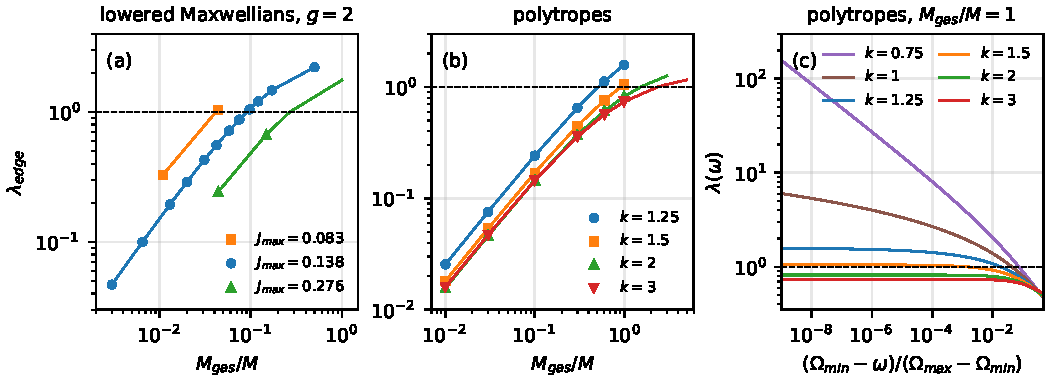
\includegraphics[width=\textwidth]{figuras/resultados_ganancia.pdf}}
\caption{Gain of the self-consistent loop. (a) The value $\lambda_{edge}$ at the edge of the frequency band as a function of the mass of the gas, for the lowered Maxwellians with $g = 2$ in the isochrone potential and three values of $J_{max}$. (b) The same for the polytropes with $k > 1$ in the Kepler potential. The symbols refer to the steady states of section~\ref{SubSec:FixedLStates}, and the lines include those which were computed in order to determine the threshold mass. (c) The gain as a function of the distance~(\ref{Eq:deltaDef}) from the edge of the band, for the polytropes with $M_{gas}/M = 1$. An oscillating mode exists if and only if the curve crosses the dashed line $\lambda = 1$.}
\label{Fig:Gain}
\end{figure}

We first verify the behavior of the gain at the edge of the band which was derived in section~\ref{SubSec:Edge}. Figure~\ref{Fig:Gain}(c) shows $\lambda$ as a function of $\delta$ for the polytropes with $M_{gas}/M = 1$. For $k > 1$ the gain converges to a finite value when $\delta\to 0$, whereas for $k\leq 1$ it grows without bound. In the interval $10^{-8}\leq \delta\leq 10^{-5}$ the logarithmic derivative $d\log\lambda/d\log\delta$ lies between $-0.261$ and $-0.252$ for $k = 0.75$, and $d\lambda/d\log(1/\delta)$ lies between $0.288$ and $0.290$ for $k = 1$, which corresponds to the laws $\delta^{k-1}$ and $|\log\delta|$, respectively. For $k > 1$, the local exponent $d\log(\lambda_{edge} - \lambda)/d\log\delta$ in the same interval lies between $0.249$ and $0.250$ for $k = 1.25$, between $0.49$ and $0.50$ for $k = 1.5$, between $0.92$ and $0.95$ for $k = 2$, and it is equal to $1.000$ for $k = 3$, in agreement with the exponent $\min\{ k-1,1 \}$ and with the logarithmic correction for $k = 2$.

Next, we consider the dependency of $\lambda_{edge}$ on the mass of the gas, which is shown in Figs.~\ref{Fig:Gain}(a) and (b). For small masses $\lambda_{edge}$ is proportional to $M_{gas}/M$, as explained in section~\ref{SubSec:Edge}: the ratio between both quantities is $15.6$ for the lowered Maxwellians with $g = 2$ and $J_{max} = 0.138$, and $2.55$, $1.81$, $1.57$ and $1.60$ for the polytropes with $k = 1.25$, $1.5$, $2$ and $3$, respectively. For larger masses the growth is slower, since the frequencies of the orbits increase with the mass of the gas; for the lowered Maxwellian with $M_{gas}/M = 0.5$ the ratio has decreased to $4.4$. Nevertheless, in all the cases $\lambda_{edge}$ increases monotonically with the mass and reaches the value one at a threshold mass. We have determined it by solving the equation $\lambda_{edge} = 1$ with a bracketing root finder, computing a self-consistent steady state for each trial value of the mass. The results are given in Table~\ref{Tab:Threshold}.

\begin{table}[htp]
\begin{center}
\begin{tabular}{ll|c|cc}
\hline\hline
 & & threshold $M_{gas}/M$ & $\Omega_{min}$ & $\Omega_{max}$ \\
\hline
lowered Maxwellian, $g = 2$ & $J_{max} = 0.083$ & $0.0416$ & $0.0705$ & $0.0807$ \\
 & $J_{max} = 0.138$ & $0.0906$ & $0.0719$ & $0.0889$ \\
 & $J_{max} = 0.276$ & $0.268$ & $0.0794$ & $0.1150$ \\
\hline
polytrope & $k = 1.25$ & $0.514$ & $0.0989$ & $0.2057$ \\
 & $k = 1.5$ & $0.920$ & $0.1473$ & $0.2935$ \\
 & $k = 2$ & $1.53$ & $0.2390$ & $0.4737$ \\
 & $k = 3$ & $2.38$ & $0.4095$ & $0.8526$ \\
\hline\hline
\end{tabular}
\end{center}
\caption{Threshold mass, defined by the condition $\lambda_{edge} = 1$, above which an oscillating mode with frequency below the band exists, and frequency band of the steady state at the threshold. For the lowered Maxwellians with $g\leq 1$ and for the polytropes with $k\leq 1$, $\lambda_{edge}$ is infinite and a mode exists for any mass.}
\label{Tab:Threshold}
\end{table}

For the lowered Maxwellians with $g = 2$ and $J_{max} = 0.138$ the threshold is $M_{gas}/M = 0.0906$. It decreases to $0.0416$ when the support of the DF is narrowed to $J_{max} = 0.083$, and it increases to $0.268$ for $J_{max} = 0.276$. For the polytropes the threshold is much larger: it is $0.514$ for $k = 1.25$ and $0.920$ for $k = 1.5$, and for $k = 2$ and $k = 3$ an oscillating mode only exists when the gas is more massive than the central object, namely for $M_{gas}/M > 1.53$ and $M_{gas}/M > 2.38$, respectively. The difference between the two families can be attributed to the width of the frequency band, which is much larger for the polytropes: the narrower the band, the smaller the perturbation of the potential which is required in order to keep the orbits in phase. For the same reason, within the first family the threshold grows with $J_{max}$.

A threshold of this kind was found by Louis~\cite{pL92} for sequences of one-dimensional polytropes and King models, whose fundamental breathing mode enters the band at a critical value of the polytropic index and of the depth of the central potential, respectively. For the polytropes in the Kepler potential, the results of Ref.~\cite{mHgRmScS25} hold when the mass of the gas is sufficiently small. Table~\ref{Tab:Threshold} shows how small it has to be for the family considered here: for $k = 1.25$, for instance, the perturbations can only be damped as long as $M_{gas}/M < 0.514$.

At a fixed mass, the existence of the mode is controlled by the behavior of the DF at the edge. For the lowered Maxwellians with $J_{max} = 0.138$ and masses in the range $0.074\leq M_{gas}/M\leq 0.078$ we obtain $\lambda_{edge} = 0.772$, $0.874$ and $1.051$ for $g = 3$, $2$ and $1.5$, respectively, and for $g\leq 1$ it is infinite; likewise, for the polytropes with $M_{gas}/M = 1$, $\lambda_{edge}$ increases from $0.738$ for $k = 3$ to $1.583$ for $k = 1.25$ (see Table~\ref{Tab:SteadyStates}). Hence, the less regular the DF is at the edge of its support, the larger is the gain. This is the quantitative counterpart of the observation of Ref.~\cite{mW91} that a sharp edge favors the existence of an oscillating mode.

When $\lambda_{edge} > 1$, the frequency of the mode follows from Eq.~(\ref{Eq:ModeFrequency}). Slightly above the threshold it lies just below the band, as is the case for the modes of the one-dimensional slab~\cite{mW91,pL92}: $\delta_d = 0.012$ for the lowered Maxwellian with $M_{gas}/M = 0.097$, and $\delta_d = 1.5\times 10^{-3}$ for the polytrope with $k = 1.5$ and $M_{gas}/M = 1$. As the mass increases, the mode separates from the band; for the lowered Maxwellians we find $\delta_d = 0.072$, $0.19$ and $0.59$ for $M_{gas}/M = 0.121$, $0.17$ and $0.5$, respectively. The frequencies $\omega_d$ are listed in Table~\ref{Tab:Modes} below.

For $k\leq 1$ an oscillating mode exists for any mass of the gas. However, when the mass is small its frequency lies extremely close to $\Omega_{min}$, as anticipated in Eq.~(\ref{Eq:Binding}). For the polytropes with $k = 0.75$ we find $\delta_d = 2.0\times 10^{-8}$, $1.5\times 10^{-6}$, $1.3\times 10^{-4}$, $4.4\times 10^{-3}$, $0.027$ and $0.075$ for $M_{gas}/M = 0.01$, $0.03$, $0.1$, $0.3$, $0.6$ and $1$, respectively. For $k = 1$ the corresponding values are $\delta_d = 4.1\times 10^{-11}$, $1.6\times 10^{-4}$, $8.5\times 10^{-3}$ and $0.044$ for $M_{gas}/M = 0.1$, $0.3$, $0.6$ and $1$, whereas for $M_{gas}/M = 0.03$ and $0.01$ the gain is still smaller than one at $\delta = 10^{-12}$, where $\lambda = 0.36$ and $0.12$, respectively; in these two cases the extrapolation with the logarithmic law yields $\delta_d\approx 10^{-33}$ and $\delta_d\approx 10^{-98}$. The scaling~(\ref{Eq:Binding}) is most clearly seen for the lowered Maxwellians with $g = 0.75$, for which $\delta_d = 4.3\times 10^{-6}$ and $3.9\times 10^{-4}$ for $M_{gas}/M = 0.0070$ and $0.0215$: the ratio between these values is $90$, compared to the factor $(0.0215/0.0070)^4 = 89$ predicted by Eq.~(\ref{Eq:Binding}). We conclude that for the steady states with $k\leq 1$ and small mass, to which the existence result of Ref.~\cite{mHgRmScS25} refers, the oscillating mode is present but cannot be resolved in a time evolution: for $k = 0.75$ and $M_{gas}/M = 0.01$ the time $2\pi/(\Omega_{min} - \omega_d)$ which would be required for this is $4\times 10^9$. A similar difficulty in classifying, by means of time evolutions, the steady states which lie close to the threshold is reported in Ref.~\cite{cS24} for isotropic polytropes.


\subsection{Decay of the perturbation below the threshold}
\label{SubSec:FixedLDamped}

We now turn to the time evolution of the perturbation~(\ref{Eq:InitialData}), starting with the steady states for which $\lambda_{edge} < 1$.

\begin{figure}[htp]
\centerline{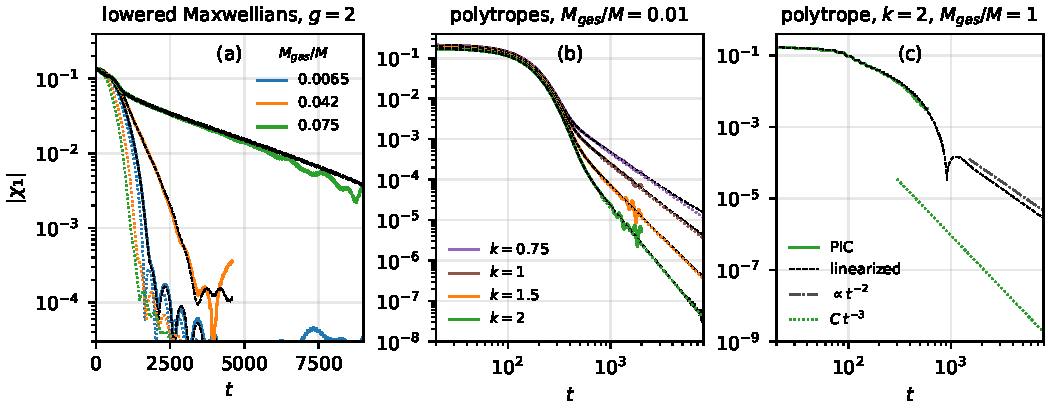
\includegraphics[width=\textwidth]{figuras/resultados_amortiguado.pdf}}
\caption{Response of the gas to the perturbation~(\ref{Eq:InitialData}) for steady states without oscillating mode. (a) Lowered Maxwellians with $g = 2$ and $J_{max} = 0.138$ below the threshold mass. The solid lines are the results of the PIC simulations (with $\varepsilon = 1$, $0.065$ and $0.075$ in the order of increasing mass), the dashed lines the solutions of the linearized equations, and the dotted lines the solutions which are obtained when the self-gravity of the perturbation is omitted. (b) Polytropes with $M_{gas}/M = 0.01$. The solid lines are the results of the PIC simulations with $\varepsilon = 0.1$, which are shown for $t\leq 2000$, the dashed lines the solutions of the linearized equations, and the dotted lines the asymptotic expression~(\ref{Eq:TailChi}) for the mixing in a fixed potential. (c) Polytrope with $k = 2$ and $M_{gas}/M = 1$. Shown is the envelope of $|\chi_1|$ (largest value in a moving window of width $40$) for the PIC simulation with $\varepsilon = 0.1$, up to $t = 600$, and for the solution of the linearized equations with $N_J = 3200$. The dash-dotted line is proportional to $t^{-2}$, and the dotted line is the expression~(\ref{Eq:TailChi}).}
\label{Fig:Damped}
\end{figure}

Figure~\ref{Fig:Damped}(a) shows the function $|\chi_1(t)|$ for the lowered Maxwellians with $M_{gas}/M = 0.0065$, $0.042$ and $0.075$, for which $\lambda_{edge} = 0.100$, $0.555$ and $0.874$, respectively. In each case we show the result of the PIC simulation, the solution of the linearized equations~(\ref{Eq:LinVlasov},\ref{Eq:LinPoisson}), and the solution of Eq.~(\ref{Eq:LinVlasov}) without its third term. The latter describes the mixing of the perturbation in the fixed potential $\Phi_{eq}$ of the steady state, when its own gravitational field is neglected, and it is given by Eq.~(\ref{Eq:hnFree}) with the frequencies $\Omega(J)$ which belong to $\Phi_{eq}$. In this case $|\chi_1|$ decays faster than exponentially and falls below one percent of its initial value at $t = 1510$, $1280$ and $1130$ for the three masses. The self-gravity of the perturbation delays the decay: when it is taken into account, the same level is reached at $t = 1650$, $2650$ and $11300$, respectively. (A delay of the phase mixing by self-gravity has also been found in $N$-body simulations of the vertical motion in a galactic disk~\cite{tAtA26}.) Hence, for the smallest mass the response is close to the one of the mixing in a fixed potential, whereas for $M_{gas}/M = 0.075$ the decay is ten times slower.

For $M_{gas}/M = 0.075$ the decay is exponential over more than two orders of magnitude, and the response is a damped oscillation of the form discussed at the end of section~\ref{SubSec:Edge}. Applying the method of section~\ref{SubSec:Fits} to the interval $2000\leq t\leq 4000$ we obtain $\omega = 0.07021\pm 6\times 10^{-5}$ and $\gamma = (3.4\pm 0.2)\times 10^{-4}$ from the solution of the linearized equations, and $\omega = 0.07028\pm 4\times 10^{-6}$ and $\gamma = (3.48\pm 0.06)\times 10^{-4}$ from the PIC simulation; in the intervals $1000\leq t\leq 2500$ and $4000\leq t\leq 7900$ the damping rate of the linearized solution is $(3.5\pm 0.6)\times 10^{-4}$ and $(3.7\pm 0.4)\times 10^{-4}$, respectively. The frequency lies inside the band, at $3$ percent of its width above the lower edge. For $t\gtrsim 1.4\times 10^4$, when the linearized solution has decreased by a factor of $300$, its decay becomes slower, which marks the transition to the algebraic tail. For $M_{gas}/M = 0.058$, where $\lambda_{edge} = 0.720$, the solution of the linearized equations yields $\omega = 0.0686$ and $\gamma = (1.1\pm 0.1)\times 10^{-3}$ in the interval $1300\leq t\leq 3900$, and the frequency lies $7$ percent of the width of the band above its lower edge. Therefore, as the threshold is approached from below, the frequency of the damped oscillation approaches the edge of the band and its damping rate tends to zero; above the threshold it becomes the oscillating mode which is analyzed in the next subsection. This is the behavior which was described by Louis~\cite{pL92} for the one-dimensional slab, where the modes that enter the band continue as density waves whose damping rate is very small close to its lower edge, and it corresponds to the divergence of the damping time at the threshold which is found for bunched beams~\cite{iKtAeS21}. For $M_{gas}/M = 0.042$ and $0.0065$, in contrast, there is no interval in which the response is described by a single exponential function: for $M_{gas}/M = 0.042$ the rates which are obtained from the linearized solution in the consecutive intervals $460\leq t\leq 1380$ and $1380\leq t\leq 2760$ are $1.3\times 10^{-3}$ and $2.6\times 10^{-3}$.

In the three cases the PIC simulations reproduce the solutions of the linearized equations as long as the response exceeds the fluctuations of the reference simulation. In terms of the quantity~(\ref{Eq:kappa}), the ratio of the amplitudes lies between $1.000$ and $1.012$ for $M_{gas}/M = 0.0065$ and $555\leq t_0\leq 1665$, an interval at whose end $|\chi_1|$ has decreased to $8\times 10^{-3}$ of its initial value, between $0.998$ and $1.000$ for $M_{gas}/M = 0.042$ and $460\leq t_0\leq 1380$, and between $0.992$ and $0.997$ for $M_{gas}/M = 0.075$ and $1000\leq t_0\leq 2500$. In the last case $|\kappa|$ decreases to $0.96$ at $t_0 = 4000$ and to $0.93$ at $t_0 = 5000$. These values change by less than one percent when the number of particles is multiplied by four or the time step is halved; the difference is an effect of the finite amplitude of the perturbation, see section~\ref{SubSec:FixedLTrapping}.

Next, we consider the polytropes with $M_{gas}/M = 0.01$, which is the regime to which the results of Ref.~\cite{mHgRmScS25} refer. In this case the gain is small, except when $k\leq 1$ and the frequency is extremely close to the edge of the band: for $\delta\geq 10^{-3}$ it does not exceed $0.06$. Consequently, the response is dominated by mixing, and its behavior for large times is determined by the edge of the support of the DF. For the mixing in the fixed potential $\Phi_{eq}$, Eq.~(\ref{Eq:Tail}) applies with $\hat{F}_1 = \mathcal{F}_{0,eq}\, s/2$, which according to Eq.~(\ref{Eq:PolytropeEdge}) corresponds to $g(J_{max}) = \alpha\,\Omega_{min}^k B(J_{max})/2$ in Eq.~(\ref{Eq:EdgeBehavior}), and one obtains
\begin{equation}
|\chi_1(t)|\simeq \frac{C}{t^{k+1}},\qquad
C := \frac{\Gamma(k+1)\,\alpha\,\Omega_{min}^k B(J_{max})}{2\,|\Omega'(J_{max})|^{k+1}\int_0^{J_{max}} \mathcal{F}_{0,eq}(J) B(J)\, dJ},\qquad t\to \infty.
\label{Eq:TailChi}
\end{equation}
We have verified this expression by solving Eq.~(\ref{Eq:LinVlasov}) without its third term on a lattice with $N_J = 3200$ rows. The envelope of the resulting function $|\chi_1(t)|$ exceeds the right-hand side of Eq.~(\ref{Eq:TailChi}) by $8$, $9$, $12$ and $14$ percent at $t = 2000$ and by $4$, $4$, $5$ and $6$ percent at $t = 4000$ for $k = 0.75$, $1$, $1.5$ and $2$, respectively, and the results for $N_J = 1600$ agree with these values to within $0.3$ percent. The difference decreases in time approximately like $1/t$, as expected for the next term of the asymptotic expansion. (For $k = 2$ this only holds up to $t\approx 5000$; afterwards the solution approaches its numerical floor, which is of the order of $10^{-7}|\chi_1(0)|$.)

The self-gravity of the perturbation modifies this behavior. To see how, we expand $\delta\mathcal{F}_0$ and $\delta\Phi(t,r(Q,J))$ in Fourier series with respect to $Q$, with coefficients $\delta\hat{F}_n(t,J)$ and $\phi_n(t,J)$, respectively. Equation~(\ref{Eq:LinVlasov}) then yields $\partial_t\delta\hat{F}_n + in\Omega\,\delta\hat{F}_n = in\,\mathcal{F}_{0,eq}'\phi_n$, whose solution is
\begin{equation}
\delta\hat{F}_n(t,J) = e^{-in\Omega(J)t}\left[ \delta\hat{F}_n(0,J) + in\,\mathcal{F}_{0,eq}'(J)\,\hat{\Phi}_n(t,J) \right],\qquad
\hat{\Phi}_n(t,J) := \int\limits_0^t \phi_n(t',J) e^{in\Omega(J)t'} dt'.
\label{Eq:Duhamel}
\end{equation}
Hence, the perturbation evolves like in a fixed potential, but with an effective initial datum which accumulates the action of the perturbed potential on each orbit. The important point is that $\mathcal{F}_{0,eq}'$ vanishes like $(J_{max} - J)^{k-1}$ at the edge of the support, that is, one power more slowly than the initial perturbation. Suppose that $k > 1$ and that $\hat{\Phi}_1(t,J_{max})$ converges to a limit $\hat{\Phi}_\infty\neq 0$ for $t\to \infty$. Then, the argument which leads to Eq.~(\ref{Eq:Tail}), applied to both terms on the right-hand side of Eq.~(\ref{Eq:Duhamel}), gives
\begin{equation}
\chi_1(t)\simeq \chi_1^{mix}(t)\left[ 1 + 2|\Omega'(J_{max})|\,\hat{\Phi}_\infty\, t \right],
\label{Eq:TailSG}
\end{equation}
where $\chi_1^{mix}$ denotes the asymptotic expression for the mixing in the fixed potential, whose magnitude is given by Eq.~(\ref{Eq:TailChi}). Therefore, for times which are large compared to $t_\times := (2|\Omega'(J_{max})||\hat{\Phi}_\infty|)^{-1}$ the response decays like $t^{-k}$ instead of $t^{-(k+1)}$: the self-gravity of the perturbation reduces the exponent of the algebraic tail by one. In the derivation of Eq.~(\ref{Eq:TailSG}) we have treated $\hat{\Phi}_1(t,J)$ as a regular function of $J$ which is independent of $t$ at late times. This neglects the potential which is generated by the tail itself; hence, the amplitude of the second term is only correct to leading order in $M_{gas}/M$.

The exponent $-k$ can be understood in two ways. First, the second term in Eq.~(\ref{Eq:Duhamel}) is a perturbation which is proportional to $\mathcal{F}_{0,eq}'$, and for the mixing of such perturbations in a fixed potential the estimates of Ref.~\cite{mHgRmScS24} give the decay rate $t^{-\min\{ 2,k \}}$ for the time derivative of the potential. Second, in the Laplace representation of Refs.~\cite{jBaOyY11,jByY13} the tail is determined by the strongest singularity on the real axis of either the response function, which contains $\mathcal{F}_{0,eq}'$ and behaves like $(\omega - \Omega_{min})^{k-1}$ at the edge of the band, or the transform of the initial perturbation, which behaves like $(\omega - \Omega_{min})^k$ for the perturbation~(\ref{Eq:InitialData}), in both cases with a logarithmic factor when the exponent is an integer. Hence, the exponent $-k$ is not new as a decay rate. What the present analysis adds is that the self-gravity of the perturbation converts the tail $t^{-(k+1)}$ of a perturbation which is proportional to the DF of the steady state into $t^{-k}$, together with the time $t_\times$ at which this occurs and the numerical evidence given below. We are not aware of quantitative results on the decay of the solutions of the full linearized system for steady states of this kind; see the remarks in Ref.~\cite{cS24} and, for steady states with a distribution of angular momenta around a point mass, Ref.~\cite{mHmS25}. \EJ{The derivation of Eq.~(\ref{Eq:TailSG}) is formal and should be checked by Olivier. The Laplace representation would also give the amplitude of the tail beyond the leading order in $M_{gas}/M$; this has not been done.}

The solutions of the full linearized equations for $M_{gas}/M = 0.01$ are shown in Fig.~\ref{Fig:Damped}(b). For $k = 1.5$ and $k = 2$ the function $\hat{\Phi}_1(t,J_{max})$, which we compute from the potential along the outermost rows of the lattice, changes by less than half a percent for $t\geq 2000$; its magnitude is $2.5\times 10^{-4}$ and $1.45\times 10^{-4}$, respectively, which corresponds to $t_\times = 3.5\times 10^4$ and $6.0\times 10^4$, and its phase differs from $\pi/2$ by less than $0.01$, such that the two terms in Eq.~(\ref{Eq:TailSG}) add in quadrature. Consequently, at $t = 8000$ the second term only increases the magnitude of the response by three and one percent, respectively, and in the time span considered here the tail follows the law of the mixing in a fixed potential: the exponents which are obtained from a fit of the envelope in the interval $2000\leq t\leq 4000$ are $-2.58$ and $-3.10$, with and without self-gravity. (At these times the exponents still differ from $-(k+1)$ because of the correction of the order $1/t$ mentioned above.) The ratio between the envelopes with and without self-gravity is almost constant: for $1000\leq t\leq 4000$ it lies between $1.04$ and $1.06$ for $k = 1.5$ and between $1.03$ and $1.04$ for $k = 2$.

For $k\leq 1$ the situation is different, since $\hat{\Phi}_1(t,J_{max})$ does not converge. For $k = 0.75$ its magnitude grows from $7.9\times 10^{-4}$ at $t = 2000$ to $8.2\times 10^{-4}$ at $t = 8000$, and the second term in Eq.~(\ref{Eq:TailSG}), evaluated with $\hat{\Phi}_1(t,J_{max})$ in place of $\hat{\Phi}_\infty$, has the magnitude $0.18$, $0.37$ and $0.75$ at $t = 2000$, $4000$ and $8000$. This term accounts for the difference with respect to the mixing in a fixed potential: the ratio between the envelopes with and without self-gravity grows from $1.06$ at $t = 2000$ to $1.13$ at $t = 4000$ and $1.35$ at $t = 8000$, and the quotient between the envelope and the right-hand side of Eq.~(\ref{Eq:TailChi}) from $1.13$ to $1.38$, whereas the quotient between the envelope and the magnitude of the right-hand side of Eq.~(\ref{Eq:TailSG}) stays between $1.11$ and $1.15$ in the whole interval $2000\leq t\leq 8000$. For $k = 1$ the second term has the magnitude $0.12$, $0.24$ and $0.47$ at the same times, and the ratio between the envelopes grows from $1.06$ to $1.09$ and $1.19$. Accordingly, the exponents in $2000\leq t\leq 4000$ are $-1.72$ for $k = 0.75$ and $-2.02$ for $k = 1$, compared to $-1.80$ and $-2.06$ without self-gravity. This slow growth is the only trace of the oscillating mode which we find for these steady states: as shown in the previous subsection, the mode itself lies at $\delta_d = 2.0\times 10^{-8}$ and $\delta_d\approx 10^{-98}$ from the edge. Therefore, over the time span considered here the perturbation decays for all the values of $k$, approximately like $t^{-(k+1)}$, and the dichotomy between $k\leq 1$ and $k > 1$ cannot be observed.

The PIC simulations agree with the solutions of the linearized equations until the response has decreased by about three orders of magnitude. As mentioned in section~\ref{SubSec:ValResponse}, for $t\leq 2000$ the difference between both is smaller than $1.2\times 10^{-4}|\chi_1(0)|$, and for $300\leq t_0\leq 1000$ the ratio $|\kappa|$ of the amplitudes lies between $0.99$ and $1.01$ for the four values of $k$. At $t = 2000$, however, the envelope of $|\chi_1|$ itself has decreased to $6.8\times 10^{-4}|\chi_1(0)|$ for $k = 0.75$ and to $1.7\times 10^{-5}|\chi_1(0)|$ for $k = 2$. Hence, the PIC simulations confirm the decay and the onset of the tail, whereas the exponents given above rely on the linearized equations.

Finally, we consider the polytrope with $k = 2$ and $M_{gas}/M = 1$, for which $\lambda_{edge} = 0.820$. Its response is shown in Fig.~\ref{Fig:Damped}(c). It starts with a damped oscillation: a fit in the interval $100\leq t\leq 400$ gives $\omega = 0.1668\pm 0.0008$ and $\gamma = (6.4\pm 0.8)\times 10^{-3}$ for the solution of the linearized equations, and $\omega = 0.1671\pm 0.0005$ and $\gamma = (6.4\pm 0.9)\times 10^{-3}$ for the PIC simulation with $\varepsilon = 0.1$. The frequency lies $4$ percent of the width of the band above its lower edge. For $t > 1500$ the linearized solution follows an algebraic tail which oscillates with the frequency $\Omega_{min}$. The exponent which is obtained from a fit of its envelope is $-2.07$ in the interval $2000\leq t\leq 4000$ and $-2.04$ in $4000\leq t\leq 8000$ for $N_J = 3200$ ($-2.07$ and $-2.02$ for $N_J = 1600$), while the envelope decreases from $2.8\times 10^{-4}|\chi_1(0)|$ to $1.6\times 10^{-5}|\chi_1(0)|$. Hence, for this mass the tail has the exponent $-k = -2$ of Eq.~(\ref{Eq:TailSG}), and not the exponent $-3$ of the mixing in a fixed potential, whose amplitude~(\ref{Eq:TailChi}) it exceeds by a factor of $400$ at $t = 2000$ and of $1500$ at $t = 8000$. In this case $t_\times = 65$. As expected, for $M_{gas}/M = 1$ Eq.~(\ref{Eq:TailSG}) does not reproduce the amplitude of the tail, which is about $13$ times larger than the one which results from the computed value $|\hat{\Phi}_\infty| = 0.047$. The same change of the exponent is found for the polytrope with $k = 1.5$ and $M_{gas}/M = 0.6$, for which $\lambda_{edge} = 0.759$: in this case the exponent of the envelope of the linearized solution is $-1.54$ in the interval $2000\leq t\leq 4000$ and $-1.52$ in $4000\leq t\leq 8000$, compared to the exponent $-2.5$ of the mixing in a fixed potential. \EJ{The PIC simulation for this case has $N = 10^4$ and $\varepsilon = 0.1$. It is to be replaced by the simulations with $N = 1.024\times 10^5$ and $\varepsilon = 0.03$ and $0.1$ which have been run on the cluster and whose analysis is pending.}


\subsection{Oscillating modes above the threshold}
\label{SubSec:FixedLModes}

\begin{figure}[htp]
\centerline{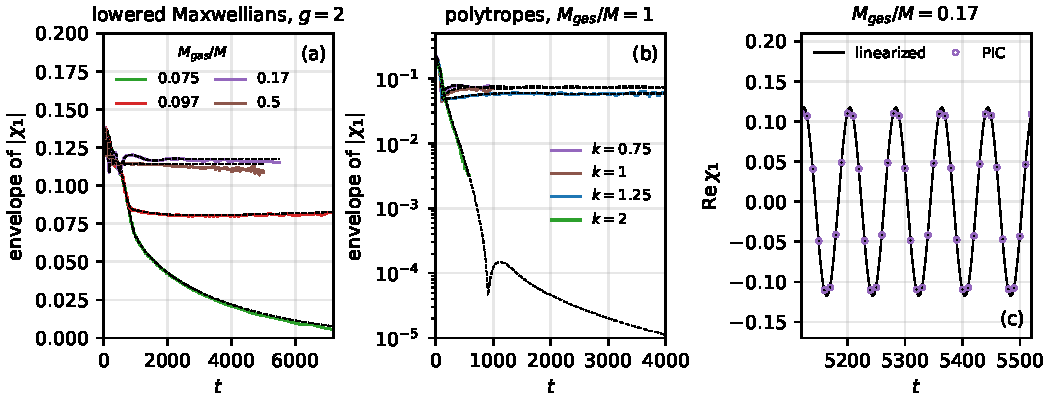
\includegraphics[width=\textwidth]{figuras/resultados_modos.pdf}}
\caption{Response of the gas for steady states above the threshold mass. (a) Envelope of $|\chi_1(t)|$ (largest value in a moving window of width $100$) for the lowered Maxwellians with $g = 2$ and $J_{max} = 0.138$, obtained from the PIC simulations with $\varepsilon = 0.075$, $0.01$, $0.1$ and $0.1$ in the order of increasing mass (solid lines) and from the linearized equations (dashed lines). The case $M_{gas}/M = 0.075$, which lies below the threshold, is included for comparison. (b) The same for the polytropes with $M_{gas}/M = 1$, with a window of width $50$. The PIC simulations have $\varepsilon = 0.1$ and are shown for $t\leq 1000$ ($t\leq 600$ for $k = 2$), except for $k = 1.25$, where $\varepsilon = 0.01$ and $N = 1.024\times 10^5$. (c) Real part of $\chi_1$ at the end of the simulation for the lowered Maxwellian with $M_{gas}/M = 0.17$.}
\label{Fig:Modes}
\end{figure}

When $\lambda_{edge} > 1$ the response does not decay. This is shown in Figs.~\ref{Fig:Modes}(a) and (b) for the lowered Maxwellians with $M_{gas}/M = 0.097$, $0.17$ and $0.5$ and for the polytropes with $k = 0.75$, $1$ and $1.25$ and $M_{gas}/M = 1$. After a transient, during which the part of the perturbation that does not belong to the mode undergoes mixing, the envelope of $|\chi_1|$ settles down to a constant value. For the lowered Maxwellians this value is $59$, $85$ and $83$ percent of $|\chi_1(0)|$ for the three masses, and for the polytropes it is $34$, $34$ and $30$ percent for the three values of $k$. The oscillation persists until the end of the linearized solutions, which comprise between $70$ and $100$ periods $2\pi/\omega_d$, and the PIC simulations follow them in amplitude as well as in phase, see Fig.~\ref{Fig:Modes}(c).

\begin{table}[htp]
\begin{center}
\begin{tabular}{ll|c|c|ccc}
\hline\hline
 & & $\Omega_{min}$ & $\delta_d$ & $\omega_d$ from Eq.~(\ref{Eq:ModeFrequency}) & linearized equations & PIC \\
\hline
lowered Maxwellian, $g = 2$ & $M_{gas}/M = 0.097$ & $0.072712$ & $0.0124$ & $0.072496$ & $0.072495$ & $0.072480$ \\
 & $M_{gas}/M = 0.17$ & $0.082745$ & $0.187$ & $0.078478$ & $0.078477$ & $0.078471$ \\
 & $M_{gas}/M = 0.5$ & $0.134193$ & $0.585$ & $0.104856$ & $0.104875$ & $0.104823$ \\
\hline
polytrope, $M_{gas}/M = 1$ & $k = 0.75$ & $0.151589$ & $0.0750$ & $0.141686$ & $0.141690$ & $0.14157$ \\
 & $k = 1$ & $0.153987$ & $0.0439$ & $0.147851$ & $0.147835$ & $0.14776$ \\
 & $k = 1.25$ & $0.156012$ & $0.0187$ & $0.153259$ & $0.153252$ & $0.153212$ \\
 & $k = 1.5$ & $0.157741$ & $0.00147$ & $0.157515$ & $0.157514$ & -- \\
\hline\hline
\end{tabular}
\end{center}
\caption{Frequency of the oscillating mode obtained from three different methods: the equation $\lambda(\omega_d) = 1$, a fit of the solution of the linearized equations, and a fit of the function $\chi_1(t)$ of the PIC simulations, both with the method of section~\ref{SubSec:Fits}. For the lowered Maxwellians the fits refer to the second half of the time span of the simulations, which extend to $t = 7200$, $5520$ and $5000$ and have the amplitudes $\varepsilon = 0.01$, $0.1$ and $0.1$, respectively. For the polytropes, the linearized solutions are fitted in the interval $1000\leq t\leq 4000$ ($8000\leq t\leq 14000$ for $k = 1.5$) and the PIC simulations in $300\leq t\leq 1000$ for $k = 0.75$ and $k = 1$ ($N = 10^4$, $\varepsilon = 0.1$) and in $500\leq t\leq 3900$ for $k = 1.25$ ($N = 1.024\times 10^5$, $\varepsilon = 0.01$).}
\label{Tab:Modes}
\end{table}

The frequencies of the oscillation are compared in Table~\ref{Tab:Modes}. Those which are obtained from the solutions of the linearized equations with the method of section~\ref{SubSec:Fits} agree with the roots of the equation $\lambda(\omega_d) = 1$ to within $2\times 10^{-5}$, that is, to within $2\times 10^{-4}$ in relative terms, and the damping rates which result from the same fits are smaller than $5\times 10^{-6}$ in magnitude, with either sign. The frequencies of the PIC simulations lie between $7\times 10^{-6}$ and $5\times 10^{-5}$ below $\omega_d$, except for the two simulations with $\varepsilon = 0.1$ and $N = 10^4$ of the polytropes, where the difference is about $10^{-4}$. The latter is consistent with the slight decrease of the frequency with the amplitude of the perturbation which was found in section~\ref{SubSec:ValResponse}. In all the cases the frequency of the oscillation lies below $\Omega_{min}$, and the distance between both is resolved by the three methods. An agreement of this kind between the frequencies predicted by the linear theory and those measured in $N$-body simulations was obtained for the modes of the one-dimensional slab in Refs.~\cite{mW91,pL92}. Together with the results of the previous subsection this confirms the criterion of section~\ref{SubSec:Gain}: for the lowered Maxwellians with $g = 2$ and $J_{max} = 0.138$ the response is damped for $M_{gas}/M = 0.075$ and oscillates without damping for $M_{gas}/M = 0.097$, in accordance with the threshold $0.0906$ of Table~\ref{Tab:Threshold}, and for the polytropes with $M_{gas}/M = 1$ it oscillates for $k\leq 1.5$ and is damped for $k = 2$. \EJ{The PIC values for $k = 0.75$ and $k = 1$ are to be replaced by those of the simulations with $N = 1.024\times 10^5$ and $\varepsilon = 0.03$ which have been run on the cluster and whose analysis is pending.}

The polytrope with $k = 1.5$ and $M_{gas}/M = 1$ lies only slightly above the threshold mass $0.920$, and its mode is located at $\delta_d = 1.5\times 10^{-3}$. As discussed in section~\ref{SubSec:Edge}, in this situation a time of the order of $(\Omega_{min} - \omega_d)^{-1} = 4400$ is needed for the mode to separate from the contribution of the orbits near the edge. In fact, the envelope of the linearized solution decreases until $t\approx 4000$, from $0.031$ at $t = 500$ to $0.022$, and it has not settled down within the time span of the solutions considered so far. We have extended this solution to $t = 1.4\times 10^4$. For $4000\leq t\leq 14000$ the envelope varies slowly between $0.022$ and $0.025$, which corresponds to $12$ to $13$ percent of $|\chi_1(0)|$. The frequencies which are obtained from fits in the intervals $4000\leq t\leq 8000$ and $8000\leq t\leq 14000$ are $0.157513$ and $0.157514$, in agreement with $\omega_d = 0.157515$, and the corresponding damping rates are $7\times 10^{-6}$ and $5\times 10^{-7}$ in magnitude. A PIC simulation of this mode in the linear regime would require a much smaller amplitude than those used here, as we show next.


\subsection{Finite amplitude: trapping of the orbits near the edge}
\label{SubSec:FixedLTrapping}

In section~\ref{SubSec:ValResponse} we found that for the polytrope with $k = 1.25$ and $M_{gas}/M = 1$ the amplitude of the response falls below the one predicted by the linearized equations by an amount which depends on $\varepsilon$ and which is not a numerical artifact. In this subsection we show that this effect is caused by the gas particles near the edge of the steady state, which are trapped by the oscillating mode when its amplitude exceeds a critical value.

That the amplitude of an oscillating mode which lies close to the band is limited was observed by Weinberg~\cite{mW91} in $N$-body simulations of the one-dimensional slab: the breathing mode could not be excited beyond about three percent of the background force, and a higher mode, which lies closer to the band, only to half a percent. He attributed this limit to the nonlinear broadening of the frequency of the mode, whose wings overlap the band and are damped, and Louis~\cite{pL92} pointed out that the trapping of resonant particles leads to oscillations of the amplitude. The pendulum model which follows turns these observations into an explicit condition.

Consider the motion of a gas particle under the influence of an oscillating mode with frequency $\omega_d$. In terms of the action-angle variables of the steady state, this motion is governed by the Hamiltonian $H = E(J) + \delta\Phi(t,r(Q,J))$, see section~\ref{SubSec:Linearization}, and the expansion of section~\ref{SubSec:Gain} gives
\begin{equation}
\delta\Phi(t,r(Q,J)) = \varepsilon\sum\limits_{n\in\Integer} \phi_n(J) e^{i(nQ - \omega_d t)} + c.c.,
\label{Eq:ModePotential}
\end{equation}
where $\phi(r)$ refers to the mode which is excited by the perturbation~(\ref{Eq:InitialData}) with $\varepsilon = 1$ in the linear regime. For an orbit whose frequency $\Omega(J)$ is close to $\omega_d$, the term with $n = 1$ in Eq.~(\ref{Eq:ModePotential}) and its complex conjugate vary slowly along the unperturbed motion $Q = Q_0 + \Omega(J)t$, whereas all the other terms oscillate with frequencies which are at least of the order of $\omega_d$ and average out. Keeping only the former, writing $\phi_1(J) = |\phi_1(J)| e^{i\beta}$ and introducing the angle
\begin{equation}
\vartheta := Q - \omega_d t + \beta,
\label{Eq:thetaDef}
\end{equation}
which together with $J$ constitutes a set of canonical variables, one obtains the time-independent Hamiltonian
\begin{equation}
K(\vartheta,J) = E(J) - \omega_d J + 2\varepsilon |\phi_1(J)|\cos\vartheta.
\label{Eq:ResonantH}
\end{equation}
Let $J_r$ be the action variable of the resonant orbit, that is, $\Omega(J_r) = \omega_d$. Since $\omega_d < \Omega_{min}$ and $\Omega$ is a decreasing function, this orbit lies outside the support of the steady state, at the distance
\begin{equation}
d := J_r - J_{max}\approx \frac{\Omega_{min} - \omega_d}{|\Omega'(J_{max})|}
\label{Eq:dDef}
\end{equation}
from its edge. Expanding $E(J) - \omega_d J$ about $J = J_r$ to second order and neglecting the variation of $\phi_1$ and $\Omega'$ between $J_{max}$ and $J_r$, Eq.~(\ref{Eq:ResonantH}) yields, up to an additive constant,
\begin{equation}
K(\vartheta,J)\approx -\frac{1}{2}|\Omega'|(J - J_r)^2 + 2\varepsilon |\phi_1|\cos\vartheta,
\label{Eq:Pendulum}
\end{equation}
which is the Hamiltonian of a pendulum. Its level sets are separated into two classes by the separatrix
\begin{equation}
J = J_r\pm \Delta J_s\left| \cos\frac{\vartheta}{2} \right|,\qquad
\Delta J_s := \frac{2\omega_b}{|\Omega'|},\qquad
\omega_b := \sqrt{2\varepsilon |\phi_1| |\Omega'|}.
\label{Eq:Separatrix}
\end{equation}
A particle which lies inside the separatrix is trapped by the mode: its angle $\vartheta$ oscillates about zero, and its action variable oscillates about $J_r$ with an amplitude of up to $\Delta J_s$ and with a frequency which is equal to the bounce frequency $\omega_b$ close to the center $(\vartheta,J) = (0,J_r)$ and decreases towards the separatrix. Outside the separatrix $\vartheta$ varies monotonically. The same pendulum describes the particles which are trapped by a wave in a plasma, where it determines the nonlinear evolution of Landau damping~\cite{tO65}, and the orbits near a resonance in a galaxy~\cite{BinneyTremaine-Book}.

Initially, all the gas particles have $J\leq J_{max} < J_r$. Therefore, the effect of the mode on them depends on the ratio
\begin{equation}
s := \frac{\Delta J_s}{d} = \frac{2\omega_b}{\Omega_{min} - \omega_d}
\label{Eq:sDef}
\end{equation}
between the half-width of the separatrix and the distance of the resonance from the edge. If $s < 1$, the separatrix does not reach the support of the steady state, and none of the gas particles is trapped. Their action variables oscillate, and it follows from Eq.~(\ref{Eq:Pendulum}) that the largest value which is attained by a particle with $J = J_{max}$ at $t = 0$ is $J_+ = J_{max} + d\,( 1 - \sqrt{1 - s^2} )$. If $s > 1$, the particles close to the edge whose angle $\vartheta$ lies in a suitable interval about zero are trapped, and those which start next to the separatrix are carried to its top, such that $J_+ = J_r + \Delta J_s = J_{max} + d\,(1 + s)$. Since $\omega_b$ is proportional to $\sqrt{\varepsilon}$, the condition $s > 1$ is equivalent to
\begin{equation}
\varepsilon > \varepsilon_c := \frac{(\Omega_{min} - \omega_d)^2}{8 |\phi_1| |\Omega'|}.
\label{Eq:epsc}
\end{equation}
Hence, the closer the frequency of the mode lies to the edge of the band, the smaller is the amplitude which is required for trapping to occur.

In order to evaluate these expressions we determine $\phi_1$ from the solution of the linearized equations. To this purpose we compute the first harmonic $(1/N_Q)\sum_b \delta\Phi(t,r_{ab}) e^{-iQ_b}$ of the perturbation of the potential along the outermost row $a = N_J$ of the lattice. Since the radius is an even function of $Q$, this quantity is real, and according to Eq.~(\ref{Eq:ModePotential}) it is equal to $2\,\re[\phi_1(J) e^{-i\omega_d t}]$ once the transient has decayed. We take for $\omega_d$ the frequency of the linearized solution which is listed in Table~\ref{Tab:Modes}, and which agrees with the root of Eq.~(\ref{Eq:ModeFrequency}) to within $2\times 10^{-5}$, and we obtain $\phi_1$ from a least-squares fit of this function in an interval which comprises between $1000$ and $2000$ time units after the transient. The results are listed in Table~\ref{Tab:Pendulum}. They change by less than two percent when the fit is repeated in the subsequent interval of at least the same length, except for $k = 1.5$, where the change is $6.5$ percent, and the root mean square of the residual of the fit does not exceed $2$ percent of the one of the function ($5$ percent for $k = 1.5$).

\begin{table}[htp]
\begin{center}
\begin{tabular}{ll|cccc|cc}
\hline\hline
 & & $\Omega_{min} - \omega_d$ & $|\Omega'(J_{max})|$ & $|\phi_1|$ & $\omega_b/\sqrt{\varepsilon}$ & $\varepsilon_c$ & $J_r/J_{max}$ \\
\hline
lowered Maxwellian, $g = 2$ & $M_{gas}/M = 0.097$ & $2.17\times 10^{-4}$ & $0.0976$ & $1.60\times 10^{-5}$ & $1.77\times 10^{-3}$ & $0.0038$ & $1.016$ \\
 & $M_{gas}/M = 0.17$ & $4.27\times 10^{-3}$ & $0.1193$ & $4.16\times 10^{-5}$ & $3.15\times 10^{-3}$ & $0.46$ & $1.26$ \\
 & $M_{gas}/M = 0.5$ & $2.93\times 10^{-2}$ & $0.2306$ & $1.31\times 10^{-4}$ & $7.78\times 10^{-3}$ & $3.5$ & $1.92$ \\
\hline
polytrope, $M_{gas}/M = 1$ & $k = 0.75$ & $9.90\times 10^{-3}$ & $0.1422$ & $7.51\times 10^{-4}$ & $1.46\times 10^{-2}$ & $0.115$ & $1.100$ \\
 & $k = 1$ & $6.15\times 10^{-3}$ & $0.1475$ & $5.76\times 10^{-4}$ & $1.30\times 10^{-2}$ & $0.056$ & $1.060$ \\
 & $k = 1.25$ & $2.76\times 10^{-3}$ & $0.1520$ & $4.06\times 10^{-4}$ & $1.11\times 10^{-2}$ & $0.015$ & $1.026$ \\
 & $k = 1.5$ & $2.3\times 10^{-4}$ & $0.1557$ & $1.45\times 10^{-4}$ & $6.7\times 10^{-3}$ & $3\times 10^{-4}$ & $1.002$ \\
\hline\hline
\end{tabular}
\end{center}
\caption{Parameters of the pendulum~(\ref{Eq:Pendulum}) which describes the motion of the gas particles near the edge of the steady state in the field of the oscillating mode: distance of the frequency of the mode from the edge of the band, derivative of the frequency of the orbits and magnitude of the first harmonic of the potential of the mode at the edge (for $\varepsilon = 1$), bounce frequency, critical amplitude~(\ref{Eq:epsc}) and action variable of the resonant orbit.}
\label{Tab:Pendulum}
\end{table}

The critical amplitude varies over four orders of magnitude. For the lowered Maxwellian with $M_{gas}/M = 0.5$ it is larger than one, such that trapping does not occur for the perturbation~(\ref{Eq:InitialData}), whereas for the modes which lie close to the edge it is very small: $\varepsilon_c = 0.0038$ for the lowered Maxwellian with $M_{gas}/M = 0.097$, and $\varepsilon_c = 0.015$ and $3\times 10^{-4}$ for the polytropes with $k = 1.25$ and $k = 1.5$. In particular, of the three amplitudes $\varepsilon = 0.01$, $0.03$ and $0.1$ which were compared in section~\ref{SubSec:ValResponse} for $k = 1.25$, the first one lies below the critical amplitude ($s = 0.80$) and the other two above it ($s = 1.39$ and $2.54$).

\begin{figure}[htp]
\centerline{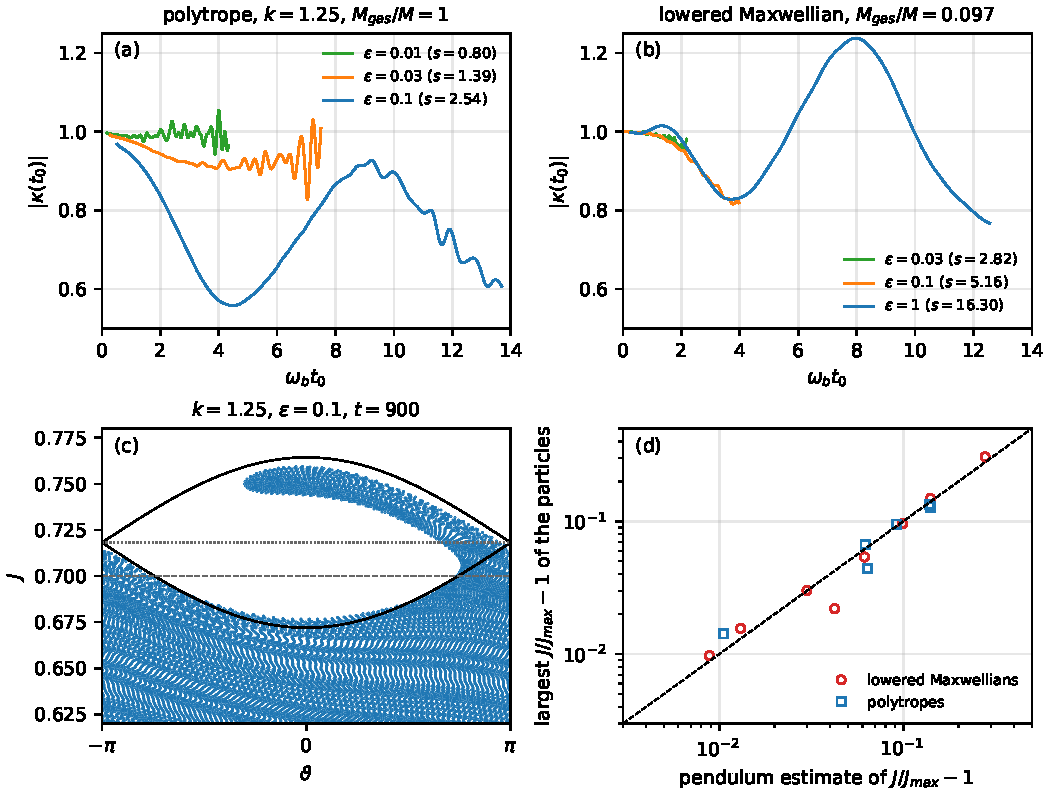
\includegraphics[width=0.85\textwidth]{figuras/resultados_atrapamiento.pdf}}
\caption{Effect of the amplitude of the perturbation on the oscillating mode. (a) Ratio $|\kappa(t_0)|$ between the amplitudes of the response obtained from the PIC code and from the linearized equations, see Eq.~(\ref{Eq:kappa}), as a function of time in units of the inverse bounce frequency, for the polytrope with $k = 1.25$ and $M_{gas}/M = 1$ and three amplitudes ($N = 1.024\times 10^5$). (b) The same for the lowered Maxwellian with $g = 2$ and $M_{gas}/M = 0.097$ ($N = 10^4$). (c) The computational particles near the edge of the steady state for the simulation with $\varepsilon = 0.1$ of panel (a) at $t = 900$, which corresponds to half a bounce period, in terms of the angle~(\ref{Eq:thetaDef}) and the action variable. The solid lines are the separatrix~(\ref{Eq:Separatrix}), the dashed line indicates $J_{max}$ and the dotted one $J_r$. (d) Largest value of the action variable attained by the computational particles in the simulations of Table~\ref{Tab:TrappingRuns}, compared to the value $J_+$ predicted by the pendulum~(\ref{Eq:Pendulum}).}
\label{Fig:Trapping}
\end{figure}

\begin{table}[htp]
\begin{center}
\begin{tabular}{ll|rc|cc|cc}
\hline\hline
 & & $\varepsilon$ & $s$ & $J_+$ (PIC) & $J_+$ (pendulum) & $\min|\kappa|$ & $\omega_b t_0$ \\
\hline
lowered Maxwellian, $g = 2$ & $M_{gas}/M = 0.097$ & $0.003$ & $0.89$ & $0.1393$ & $0.1392$ & $0.98$ & -- \\
 & & $0.01$ & $1.63$ & $0.1410$ & $0.1438$ & $0.98$ & $1.2^*$ \\
 & & $0.03$ & $2.82$ & $0.1454$ & $0.1465$ & $0.96$ & $2.1^*$ \\
 & & $0.1$ & $5.16$ & $0.1512$ & $0.1517$ & $0.82$ & $3.8^*$ \\
 & & $1$ & $16.3$ & $0.1802$ & $0.1765$ & $0.83$ & $3.7$ \\
 & $M_{gas}/M = 0.17$ & $0.1$ & $0.47$ & $0.1422$ & $0.1421$ & $0.99$ & -- \\
 & $M_{gas}/M = 0.5$ & $0.1$ & $0.17$ & $0.1402$ & $0.1398$ & $0.99$ & -- \\
 & & $1$ & $0.53$ & $0.1586$ & $0.1574$ & $1.00$ & -- \\
\hline
polytrope, $M_{gas}/M = 1$ & $k = 1.25$ & $0.01$ & $0.80$ & $0.7099$ & $0.7074$ & $0.98$ & -- \\
 & & $0.03$ & $1.39$ & $0.7467$ & $0.7435$ & $0.89$ & $5.4$ \\
 & & $0.1$ & $2.54$ & $0.7667$ & $0.7644$ & $0.56$ & $4.5$ \\
 & & $0.3$ & $4.41$ & $0.7897$ & $0.7982$ & $0.31$ & $4.1$ \\
 & $k = 1$ & $0.1$ & $1.34$ & $0.7941$ & $0.7976$ & $0.89$ & $3.6^*$ \\
 & $k = 0.75$ & $0.1$ & $0.93$ & $0.7308$ & $0.7446$ & $0.96$ & -- \\
\hline\hline
\end{tabular}
\end{center}
\caption{Simulations of steady states with an oscillating mode for different amplitudes of the perturbation: ratio~(\ref{Eq:sDef}), largest value of the action variable attained by the computational particles and its estimate $J_+$ from the pendulum~(\ref{Eq:Pendulum}), and smallest value of the ratio $|\kappa|$ between the amplitudes of the response of the PIC code and of the linearized equations. For $s > 1$ the latter refers to the interval $\omega_b t_0\leq 6$, and the last column gives the time at which it is attained; an asterisk indicates that this occurs at the end of the time span which is analyzed, such that $|\kappa|$ may decrease further. For $k = 1.25$ and $\varepsilon = 0.01$ the smallest value for $t_0\leq 2000$ is given. The simulations have $N = 10^4$ and are analyzed over their whole duration, except those of the polytropes with $k = 1.25$ and $\varepsilon\leq 0.1$, which have $N = 1.024\times 10^5$, and the remaining ones of the polytropes, which are only analyzed for $t\leq 1000$.}
\label{Tab:TrappingRuns}
\end{table}

These estimates are compared with the PIC simulations in Table~\ref{Tab:TrappingRuns} and Fig.~\ref{Fig:Trapping}. We first consider the motion of the particles. Figure~\ref{Fig:Trapping}(c) shows the computational particles with the largest values of the action variable for the polytrope with $k = 1.25$ and $\varepsilon = 0.1$ at $t = 900$, which corresponds to half a bounce period $\pi/\omega_b$. The particles which were located next to the edge with angles close to $\vartheta = 0$ have moved around the center of the island, and they reach $J = 0.76$, while the top of the separatrix lies at $J_r + \Delta J_s = 0.764$. The largest value of the action variable which is attained in the course of the simulation is $0.7099$, $0.7467$ and $0.7667$ for $\varepsilon = 0.01$, $0.03$ and $0.1$, respectively, compared to the estimates $J_+ = 0.7074$, $0.7435$ and $0.7644$; in the reference simulation it is $0.7033$. In particular, the excursion beyond $J_{max}$ grows by a factor of five between $\varepsilon = 0.01$ and $\varepsilon = 0.03$, which reflects the onset of the trapping at $\varepsilon_c = 0.015$. The same agreement is found for the remaining simulations, see Fig.~\ref{Fig:Trapping}(d): for those with $s > 1$ which extend over at least two units of $1/\omega_b$, the measured excursion $J_+ - J_{max}$ differs from the estimate by at most $12$ percent. The simulation with $\varepsilon = 0.01$ for the lowered Maxwellian with $M_{gas}/M = 0.097$ ends at $\omega_b t = 1.3$, before the trapped particles have completed half a bounce period, and in this case the excursion has only reached half of the estimate. For $s < 1$, where the excursions are small, the relative deviations are larger, up to $35$ percent. We stress that the estimate does not contain any adjustable parameter.

Next, we consider the amplitude of the response, which we compare with the one of the linearized solution by means of the quantity~(\ref{Eq:kappa}). In the simulations with $s < 1$, $|\kappa|$ stays between $0.98$ and $1.01$ for the lowered Maxwellians, and for the polytrope with $k = 1.25$ and $\varepsilon = 0.01$ it lies between $0.977$ and $1.005$ for $t_0\leq 2000$ (see section~\ref{SubSec:ValResponse}). For $s > 1$, in contrast, the amplitude falls below the linear one on the time scale $1/\omega_b$ and passes through a minimum at $\omega_b t_0\approx 4$, see Figs.~\ref{Fig:Trapping}(a) and (b). For the polytrope with $k = 1.25$ and $\varepsilon = 0.1$ the minimum is $0.56$ at $\omega_b t_0 = 4.5$; for $\varepsilon = 0.03$, where $s = 1.39$ is closer to the critical value, $|\kappa|$ decreases to $0.90$ at $\omega_b t_0 = 4.4$ and stays between $0.89$ and $0.95$ up to $\omega_b t_0 = 6.5$. For the lowered Maxwellian with $M_{gas}/M = 0.097$, the curves for $\varepsilon = 0.03$, $0.1$ and $1$, for which $s$ lies between $2.8$ and $16$, coincide with each other to within four percent when they are represented as functions of $\omega_b t_0$, as far as each simulation extends. In the simulation with $\varepsilon = 1$, which covers almost thirteen units of $1/\omega_b$, the minimum $|\kappa| = 0.83$ at $\omega_b t_0 = 3.7$ is followed by a maximum of $1.24$ at $\omega_b t_0 = 8.0$, after which $|\kappa|$ decreases again, to $0.77$ at the end of the simulation. Hence, the amplitude of the mode oscillates with a period which is about $1.4$ times the bounce period $2\pi/\omega_b$. Such oscillations are characteristic for a wave which interacts with trapped particles~\cite{tO65}; for the one-dimensional slab they were anticipated in Ref.~\cite{pL92}. The results for $\varepsilon = 0.1$ and $M_{gas}/M = 0.097$ do not change when the number of particles is multiplied by four or the time step is halved: at $\omega_b t_0 = 3$ we obtain $|\kappa| = 0.872$, $0.873$ and $0.872$, respectively.

The reason for the loss of amplitude is the following. According to Eq.~(\ref{Eq:ModeEq}), in the linearized theory the DF of the mode is proportional to $\mathcal{F}_{0,eq}'(J)\,\phi_1(J)/[\Omega(J) - \omega_d]$, which is largest for the orbits near the edge, where $\Omega(J) - \omega_d$ is smallest. This expression presupposes that the particles follow the unperturbed orbits. For the trapped particles this is not the case: their contribution to the density of the mode ceases to grow in phase with the potential and oscillates with the bounce period instead. Although these particles carry a very small fraction of the mass of the gas (in the simulation with $k = 1.25$ and $\varepsilon = 0.1$, the particles which reach $J > J_{max} + 0.003$ amount to $1.5\times 10^{-4} M_{gas}$), their weight in the mode is large due to the small denominator. This explanation is consistent with the fact that, at comparable values of $s$, the loss is larger for the polytrope with $k = 1.25$ than for the lowered Maxwellian with $g = 2$ (compare the rows with $s = 2.55$ and $s = 5.17$ in Table~\ref{Tab:TrappingRuns}), since in the former case the derivative of the DF vanishes more slowly at the edge. It is also in line with the analysis by Louis and Gerhard~\cite{pLoG88} of a radial oscillation of finite amplitude of the isochrone sphere, in which the orbits that are trapped around the stable resonant orbits oscillate against the perturbation and damp it, such that a self-consistent oscillation requires a DF which is depleted at the resonances. However, we do not have a quantitative theory for the depth of the minimum.

Finite amplitude effects are also present below the threshold, where the resonant orbit lies inside the support of the steady state. For the lowered Maxwellian with $M_{gas}/M = 0.075$, whose response in the linear regime is damped with the rate $\gamma = 3.4\times 10^{-4}$ (see section~\ref{SubSec:FixedLDamped}), we have performed a simulation with $\varepsilon = 0.84$ up to $t = 17200$. In this case the decay of the envelope of $|\chi_1|$ stops at $t\approx 2700$, when it has decreased to $22$ percent of its initial value. Afterwards the envelope grows to $52$ percent at $t\approx 6500$, decreases to $18$ percent at $t\approx 11500$ and grows again; the same values are obtained with four times as many particles and with half the time step up to $t = 5000$. The period of this oscillation, about $8900$, is comparable to the bounce period $2\pi/\omega_b = 7700$ which results from Eq.~(\ref{Eq:Separatrix}) with the mean amplitude of the potential in the interval $4000\leq t\leq 17200$. This is the saturation of Landau damping by the trapping of the resonant particles which was predicted by O'Neil~\cite{tO65} for a plasma wave: the damping stops once the bounce frequency exceeds the damping rate.

We conclude that the linear regime of an oscillating mode is restricted to amplitudes $\varepsilon\ll \varepsilon_c$. For the modes which emerge at the threshold this is a severe restriction, since $\varepsilon_c$ vanishes quadratically with the distance $\Omega_{min} - \omega_d$ of the mode from the band. In this sense, Eq.~(\ref{Eq:epsc}) gives an explicit expression for the amplitude at which the limitation observed in Ref.~\cite{mW91} sets in. \EJ{The simulations of this subsection for $k = 0.75$ and $k = 1$ have $N = 10^4$ and $\varepsilon = 0.1$, and their analysis is restricted to $t\leq 1000$. They are to be replaced by the simulations with $N = 1.024\times 10^5$ and $\varepsilon = 0.03$ and $0.1$ which have been run on the cluster and whose analysis is pending; according to Table~\ref{Tab:Pendulum}, $\varepsilon = 0.03$ lies below the critical amplitude in both cases.}



%%%%%%%%%%%%%%%%%%%%%%%%%%%%%%%%%%%%%%%%%%%%%
\section{Conclusions}
\label{Sec:Conclusions}
%%%%%%%%%%%%%%%%%%%%%%%%%%%%%%%%%%%%%%%%%%%%%

In these notes we have studied numerically the evolution of small perturbations of the self-consistent steady states of a spherically symmetric collisionless gas which is trapped in an external central potential, in the reduced model in which all the gas particles have the same magnitude of the angular momentum. Our analysis is based on three tools which agree with each other: a PIC code whose particles are placed on a regular lattice in the action-angle variables of the steady state and carry the perturbation in their weights, a solution of the linearized equations in the same variables, and the gain $\lambda(\omega)$ of the self-consistent loop. In this section we summarize the results and list some open problems.

Below the threshold mass at which $\lambda_{edge} = 1$, the perturbation decays. When the self-gravity of the gas is not too weak, the decay is dominated at intermediate times by a damped oscillation, the analogue of Landau damping, whose frequency lies inside the frequency band and approaches its lower edge, while the damping rate decreases, as the threshold is approached. At late times the decay is algebraic. In a fixed potential, a DF which vanishes like $(E_0 - E)^k$ at the edge of its support gives rise to a tail proportional to $t^{-(k+1)}$; the self-gravity of the perturbation reduces this exponent to $-k$ after the time $t_\times$, which we have estimated to leading order in the mass of the gas. For the polytropes with $M_{gas}/M = 0.01$ this time exceeds the time span of our simulations, whereas for $k = 2$ and $M_{gas}/M = 1$ the exponent of the tail is $-2.07$ in the interval $2000\leq t\leq 4000$ and $-2.04$ in $4000\leq t\leq 8000$.

The threshold mass depends strongly on the width of the frequency band and on the behavior of the DF at the edge of its support. For the lowered Maxwellians in the isochrone potential it lies between $0.04$ and $0.27$ times the mass which generates the external potential, depending on the width of the support of the DF, whereas for the polytropes in the Kepler potential it is $0.514$, $0.920$, $1.53$ and $2.38$ for $k = 1.25$, $1.5$, $2$ and $3$, respectively. Hence, the damping of the perturbations which has been established for small masses in Ref.~\cite{mHgRmScS25} does not extend beyond these values. For $k\leq 1$ an oscillating mode exists for any mass, but for small masses its frequency lies so close to the edge of the band that it cannot be observed in a time evolution: for $k = 0.75$ and $M_{gas}/M = 0.01$ the distance from the edge is $2\times 10^{-8}$ times the width of the band. Above the threshold the perturbation contains an oscillating mode, and its mixing is not completed. The frequency of the mode which follows from the equation $\lambda(\omega_d) = 1$ agrees with the one of the linearized solutions to within $2\times 10^{-4}$ in relative terms, and with the one of the PIC simulations to within $5\times 10^{-5}$ for small amplitudes.

The linear regime of a mode which lies close to the edge of the band is restricted to small amplitudes. Above the critical amplitude~(\ref{Eq:epsc}), which vanishes quadratically with the distance of the mode from the band, the gas particles near the edge of the steady state are trapped by the mode. A pendulum model gives the largest action variable which is reached by these particles to within $12$ percent, without adjustable parameters, and the trapping reduces the amplitude of the mode, which then oscillates with a period of about $1.4$ times the bounce period. Below the threshold, the same mechanism stops the damping of a perturbation of large amplitude, as predicted by O'Neil for plasma waves~\cite{tO65}.

The numerical methods required some care. The observables have to be computed with the action-angle variables of the total potential, since those of the external potential leave a time-independent residue which could be mistaken for an undamped mode. The quiet start on a lattice in action-angle variables reduces the noise by several orders of magnitude, but for $M_{gas}/M = 1$ its regularity is lost after $t\approx 1000$ with $10^4$ particles, and about $10^5$ particles and amplitudes $\varepsilon\leq 0.01$ are needed in order to reproduce the solutions of the linearized equations within a few percent.

Several questions remain open. The derivation of the tail $t^{-k}$ is formal, and its amplitude is only known to leading order in $M_{gas}/M$; the Laplace representation of Refs.~\cite{jBaOyY11,jByY13} would also give the amplitude beyond this order. The depth of the loss of amplitude which is caused by the trapped particles is not explained by the pendulum model. The simulations with $M_{gas}/M = 1$ and $k = 0.75$, $1$ and $2$ have to be repeated with $10^5$ particles and smaller amplitudes. Finally, the extension to a distribution of angular momenta, for which the frequency band and its edge depend also on $L$, is left for future work. \EJ{To be completed after the discussion with Olivier; reference to the companion article on initial data far from equilibrium to be added.}



%%%%%%%%%%%%%%%%%%%%%%%%%%%
%%%   ACKNOWLEDGMENTS
%%%%%%%%%%%%%%%%%%%%%%%%%%%

\acknowledgments

\EJ{To be written.}


\appendix

%%%%%%%%%%%%%%%%%%%%%%%%%%%%%%%%%%%%%%%%%%%%%
\section{Numerical computation of the action-angle variables}
\label{App:ActionAngle}
%%%%%%%%%%%%%%%%%%%%%%%%%%%%%%%%%%%%%%%%%%%%%

In this appendix we describe the numerical evaluation of the action-angle variables defined in Eqs.~(\ref{Eq:AreaFunction},\ref{Eq:TDef},\ref{Eq:JQDef}) for a potential of the form $\Phi = \Phi_{ext} + \Phi_{gas}$, in which $\Phi_{gas}$ is only known on a radial grid. This is required for the construction of the self-consistent steady states, for the generation of the initial data and for the computation of the observables $h_n(t)$.

The values of $\Phi_{gas}$ on the grid are interpolated with a natural cubic spline, and beyond the last grid point we set $\Phi_{gas} = -G M_{gas}/r$. Given a point $(r,p_r,L)$ we compute its energy $E$ from Eq.~(\ref{Eq:EDef}), locate the minimum $r_{min}(L)$ of the effective potential $V_L$, and determine the turning points $r_1 < r_{min}(L) < r_2$ by solving the equation $V_L(r) = E$ with the bisection method on either side of the minimum. The integrand in Eq.~(\ref{Eq:AreaFunction}) behaves like a square root at the turning points and the one in Eq.~(\ref{Eq:TDef}) like an inverse square root, which spoils the convergence of standard quadrature rules. We avoid this problem by means of the substitution
\begin{equation}
r = r_m + r_a\sin\theta,\qquad
r_m := \frac{r_1 + r_2}{2},\quad r_a := \frac{r_2 - r_1}{2},\qquad
-\frac{\pi}{2}\leq \theta\leq \frac{\pi}{2}.
\label{Eq:ThetaSubstitution}
\end{equation}
Since for a non-circular orbit the zeros of the function $E - V_L$ at the turning points are simple, one has $E - V_L(r) = r_a^2\cos^2\theta\, u(\theta)$ with a smooth and positive function $u$, and it follows that
\begin{equation}
A(E,L) = 2r_a^2\int\limits_{-\pi/2}^{\pi/2} \cos^2\theta\,\sqrt{2u(\theta)}\, d\theta,\qquad
T(E,L) = 2\int\limits_{-\pi/2}^{\pi/2} \frac{d\theta}{\sqrt{2u(\theta)}}.
\label{Eq:ATSmooth}
\end{equation}
Both integrands are smooth, and we evaluate the integrals with a Gauss-Legendre rule with $64$ nodes. The angle variable is obtained in the same way from
\begin{equation}
Q = \frac{2\pi}{T(E,L)}\int\limits_{-\pi/2}^{\theta(r)} \frac{d\theta'}{\sqrt{2u(\theta')}},\qquad
\theta(r) := \arcsin\left( \frac{r - r_m}{r_a} \right),
\label{Eq:QSmooth}
\end{equation}
when $p_r\geq 0$, and from $2\pi$ minus the right-hand side of Eq.~(\ref{Eq:QSmooth}) when $p_r < 0$. For the isochrone potential without self-gravity, for which the exact expressions~(\ref{Eq:AreaIsochrone},\ref{Eq:OmegaIsochrone}) are available, this procedure yields the action variable with an error of the order of $10^{-14}$ and the period with an error of the order of $10^{-11}$. Without the substitution~(\ref{Eq:ThetaSubstitution}) the corresponding errors are $2\times 10^{-6}$ and $9\times 10^{-3}$, and they only decrease like the third and the first inverse power of the number of nodes, respectively.

For the inverse map $(Q,J)\mapsto (r,p_r)$ at fixed $L$ we tabulate the function $J = A(E,L)/2\pi$ for $4000$ values of the energy between $E_{min}(L)$ and a value slightly above the cutoff energy, and obtain $E(J,L)$ by interpolation. Next, we determine the turning points and find, by bisection in $\theta$, the point of the orbit at which the time elapsed since the passage through the pericenter is equal to $QT(E,L)/2\pi$ when $Q\leq \pi$ and to $(2\pi - Q)T(E,L)/2\pi$ otherwise. This gives the radius $r$, and the momentum is $p_r = \pm\sqrt{2(E - V_L(r))}$, with the positive sign when $Q\leq \pi$. Applying the direct map to the result reproduces the points of the lattice~(\ref{Eq:Lattice}) with errors which are smaller than $10^{-8}$ in $J$ and $5\times 10^{-7}$ in $Q$. The frequency is obtained from $\Omega = 2\pi/T(E,L)$.



\bibliographystyle{unsrt}
\bibliography{refs}

\end{document}
